\documentclass[dutch]{0_dissertation}

\usepackage{float}
\usepackage{tabularx}
\addbibresource{0_ref.bib}
\usepackage[utf8]{inputenc}

\usepackage{listings}
\usepackage{xcolor}

\definecolor{codegreen}{rgb}{0,0.6,0}
\definecolor{codegray}{rgb}{0.5,0.5,0.5}
\definecolor{codepurple}{rgb}{0.58,0,0.82}
\definecolor{backcolour}{rgb}{0.95,0.95,0.92}

\lstdefinestyle{mystyle}{
    backgroundcolor=\color{backcolour},   
    commentstyle=\color{codegreen},
    keywordstyle=\color{magenta},
    numberstyle=\tiny\color{codegray},
    stringstyle=\color{codepurple},
    basicstyle=\ttfamily\footnotesize,
    breakatwhitespace=false,         
    breaklines=true,                 
    captionpos=b,                    
    keepspaces=true,                 
    numbers=left,                    
    numbersep=5pt,                  
    showspaces=false,                
    showstringspaces=false,
    showtabs=false,                  
    tabsize=2
}


\lstset{style=mystyle}
\begin{document}

\renewcommand{\contentsname}{Inhoudsopgave}

%% Specify the title. This information will be used on
%% the title page (in title/title.tex) and in the metadata of the final PDF.

\title[Ontwerpopdracht pakkethondje]{Ontwerprapport 1}

\frontmatter

%Zet hier alles neer dat voor de table of contents komt.

\begin{titlepage}

\begin{center}

%% Extra whitespace at the top.
\vspace*{\bigskipamount}

%% Print the title defined in wop3.tex.
{\makeatletter
\titlestyle\bfseries\LARGE\@title
\makeatother}

%% Print the optional subtitle.
{\makeatletter
\ifx\@subtitle\undefined\else
    \bigskip
    \titlefont\titleshape\Large\@subtitle
\fi
\makeatother}

\vspace{\baselineskip} %creates some space between titles and image

\begin{figure}[h]
    \centering
    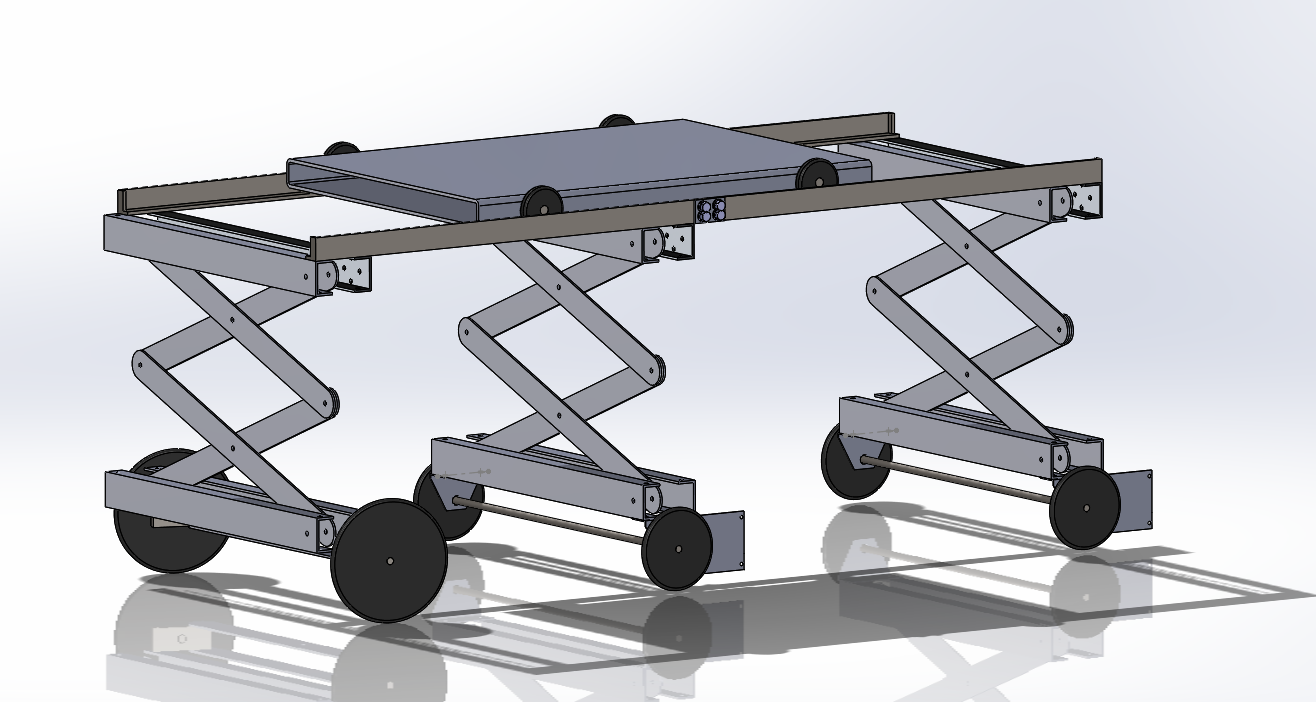
\includegraphics[height =70mm]{04_gekozenconcept/eindconcept.png}
    \label{fig:title_image}
\end{figure}


\end{center}

\begin{flushleft}

\bfseries Groepsleden: \mdseries
\begin{table}[h]
    \begin{tabular}{lll}
        Hilbert Bijzitter &  & 5112585 \\
        Robin ter Heide &  & 4812646 \\
        Max Leenstra &  &5150566 \\
        Kevin Tran &  & 4904672 \\
        Floris Kuck &  & 5112583 \\
        Beer Mook &  & 5106133
    \end{tabular}
\end{table}

 \begin{minipage}{.5\linewidth}
    \begin{flushleft}
      Vak:  Werktuigkundig ontwerpproject 3A WB1643A, Werktuigbouwkunde\\
      Studentmentor: Christopher Combes\\
      Docent: Wim van Son \\
      Docent: Regina Tange-Hoffmann
    \end{flushleft}
  \end{minipage}
  \hfill
  \begin{minipage}{.45\linewidth}
    \begin{flushright}
    Datum: \today\\
    Studiejaar: 2019 - 2020\\
    Teamnummer: WB32
    \end{flushright} 
\end{minipage}

\begin{figure}[h]
    \centering
    
\includegraphics[width = 40mm]{01_title/TUDELFT_LOGO.png}
\end{figure}
  
  
\cleardoublepage
\thispagestyle{empty}
\end{flushleft}

\clearpage
\thispagestyle{empty}
\end{titlepage}

\chapter*{Voorwoord}
\label{cha:voorwoord}
\addcontentsline{toc}{chapter}{Voorwoord}
\setheader{Voorwoord}

Het eerste jaar van de studie Werktuigbouwkunde aan de TU Delft wordt afgesloten met de  Eerstejaars Ontwerpwedstrijd. Tijdens het project dat hieraan verbonden is krijgt een groep studenten een opdracht, welke elk jaar verschilt, en moeten hier samen voor een half jaar aan werken om tot een zo goed mogelijk resultaat te komen. 

Dit jaar is de opdracht van de ontwerpwedstrijd om een ‘pakkethondje’ te bouwen, afgeleid van het welbekende meubelhondje. Het pakkethondje zou gebruikt moeten worden om het afleveren van pakketjes tot aan de deur makkelijker te maken. Dit project heeft als doelgroep de leveranciers van pakketjes. Wij, bestaande uit 6 eerstejaars studenten Werktuigbouwkunde, zijn een van vele groepjes die dit jaar meedoen met de ontwerpwedstrijd. In dit rapport is het proces besproken hoe dit project is aangepakt en tot welk ontwerp wij uiteindelijk zijn gekomen.

Tijdens het ontwerpproces hebben wij ons op verschillende manieren laten inspireren. We hebben gekeken naar hoe bepaalde dieren zich in de natuur voortbewegen over obstakels en nagedacht of dit ook in dit project zou kunnen worden toegepast. Ook hebben wij ACCREx toegepast en een morfologische kaart gebruikt om tot zoveel mogelijk deeloplossingen te komen voor de verschillende ontwerp uitdagingen.

In \cref{cha:Concept_keuze} word voor de geïnteresseerde uitgelicht hoe de verschillende deelconcepten hebben geleid tot een uiteindelijk definitief concept. Wie juist geïnteresseerd is in hoe we tot de deeloplossingen zijn gekomen voor de verschillende ontwerp uitdagingen kunnen wij verwijzen naar \cref{cha:ideeOntwikkeling}, waar de idee ontwikkeling in wordt uitgewerkt.

Tot slot willen wij nog een aantal personen bedanken van wie wij de nodige hulp hebben gehad om tot het eindproduct te komen: onze project docent Wim van Son, onze projectmentor Christopher Combes, onze Schriftelijk Rapporteren docent Regina Tange-Hoffmann en de docent van het vak WOP 3A Anton van Beek.

\vspace{\baselineskip}
Delft, \today\\
\begin{table}[h]
    \begin{tabular}{l}
        Hilbert Bijzitter\\
        Robin ter Heide\\
        Max Leenstra\\
        Kevin Tran\\
        Floris Kuck\\
        Beer Mook
    \end{tabular}
\end{table}

\vspace{\baselineskip}




\chapter*{Samenvatting}
\label{cha:Samenvatting}
\addcontentsline{toc}{chapter}{Samenvatting}
% Let op! geen verwijzingen naar paragrafen in de samenvatting. Hij moet zelfstandig leesbaar zijn

Voor de ontwerpwedstrijd van de studie Werktuigbouwkunde moesten alle eerstejaarsstudenten een pakkethondje ontwerpen. Dit pakkethondje moest een pakketje van een verhoging kunnen aannemen, daarmee over een parcours met een talud en een zelfgekozen hindernis. De zelfgekozen hindernis wordt gekozen op basis van moeilijkheid, wat extra punten oplevert. Ze zijn gemaakt van opsluitbanden en hebben een individuele afmeting van 55x145x1000 mm. Dit rapport beschrijft de het ontwerpproces, de verschillende concepten en het uiteindelijke gekozen ontwerp.

Op basis van het programma van eisen zijn er verschillende deeloplossingen in een morfologische kaart gezet. Door combinaties van deze deeloplossingen te maken zijn er 4 kansrijke concepten bedacht, welke verder zijn uitgewerkt.

Het eerste concept is de Mantis car. De Mantis car werkt door middel van grijphaken die gebaseerd zijn op hetzelfde idee als de poten van een sprinkhaan, zie \cref{fig:deeloplossing_mantis2}. De grijphaken zijn verbonden met een as, welke aangedreven wordt door een elektromotor. Hiermee kunnen de verschillende taluds worden overwonnen doordat het concept zichzelf omhoog trekt. Het voordeel van de Mantis car is dat het makkelijk te construeren is. Het nadeel is de stabiliteit van het pakketje. Deze komt tijdens het overwinnen van de taluds schuin te staan en dit kan verschillende problemen veroorzaken.

\begin{figure}[h]
    \centering
    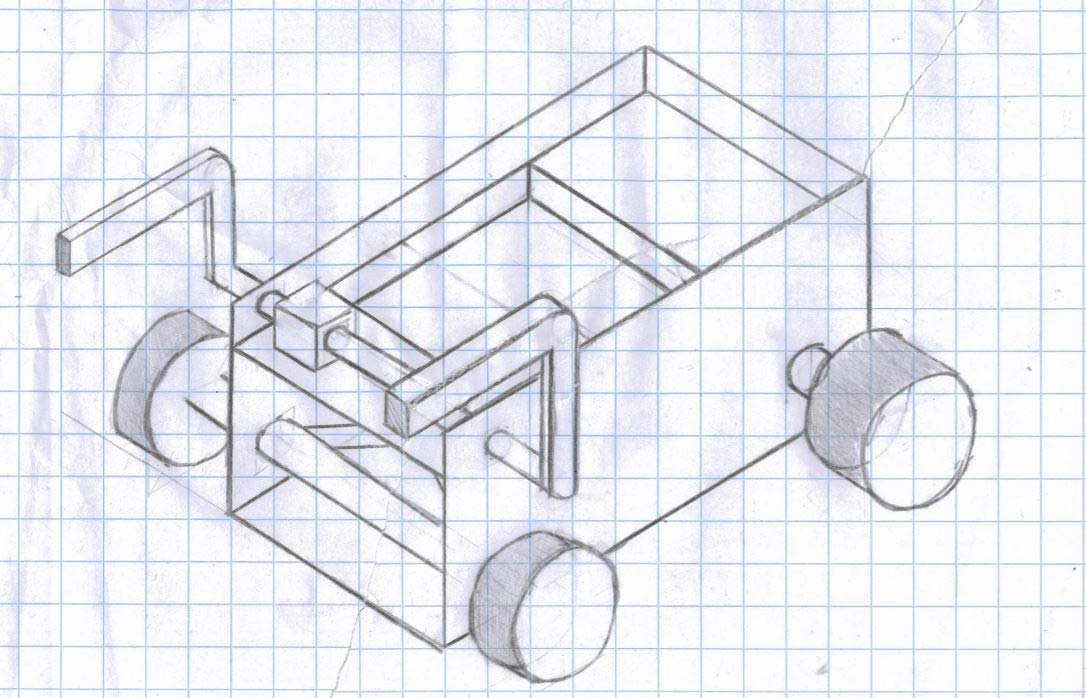
\includegraphics[width = 80mm]{04_idee_ontwikkeling/deeloplossing_mantis.JPG}
    \caption{Concept 1, de Mantis car}
    \label{fig:deeloplossing_mantis2}
\end{figure}

Het tweede concept is de Uitschuiver. De Uitschuiver heeft 2 delen welke afzonderlijk kunnen worden ingetrokken en uitgeschoven, zie \cref{fig:isom_uitschuiver2}. De Uitschuiver heeft ook inklapbare pootjes, welke kunnen worden ingetrokken. Wanneer deze worden ingetrokken kan het voorste deel van de Uitschuiver over het talud heen worden geschoven, en zo kan het obstakel worden overwonnen. Het zwaartepunt kan worden veranderd door het pakketje heen en weer te schuiven. Een voordeel van dit concept is dat de werking voorspelbaar is. Dit omdat het talud niet wordt aangeraakt bij dit concept en het model niet wordt belast op krachten die niet van tevoren te voorspellen zijn. Een nadeel is de maakbaarheid, omdat het uitschuifmechanisme in combinatie met de het schuiven van het pakketje een gecompliceerd systeem is.

\begin{figure}[!htp]
    \centering
    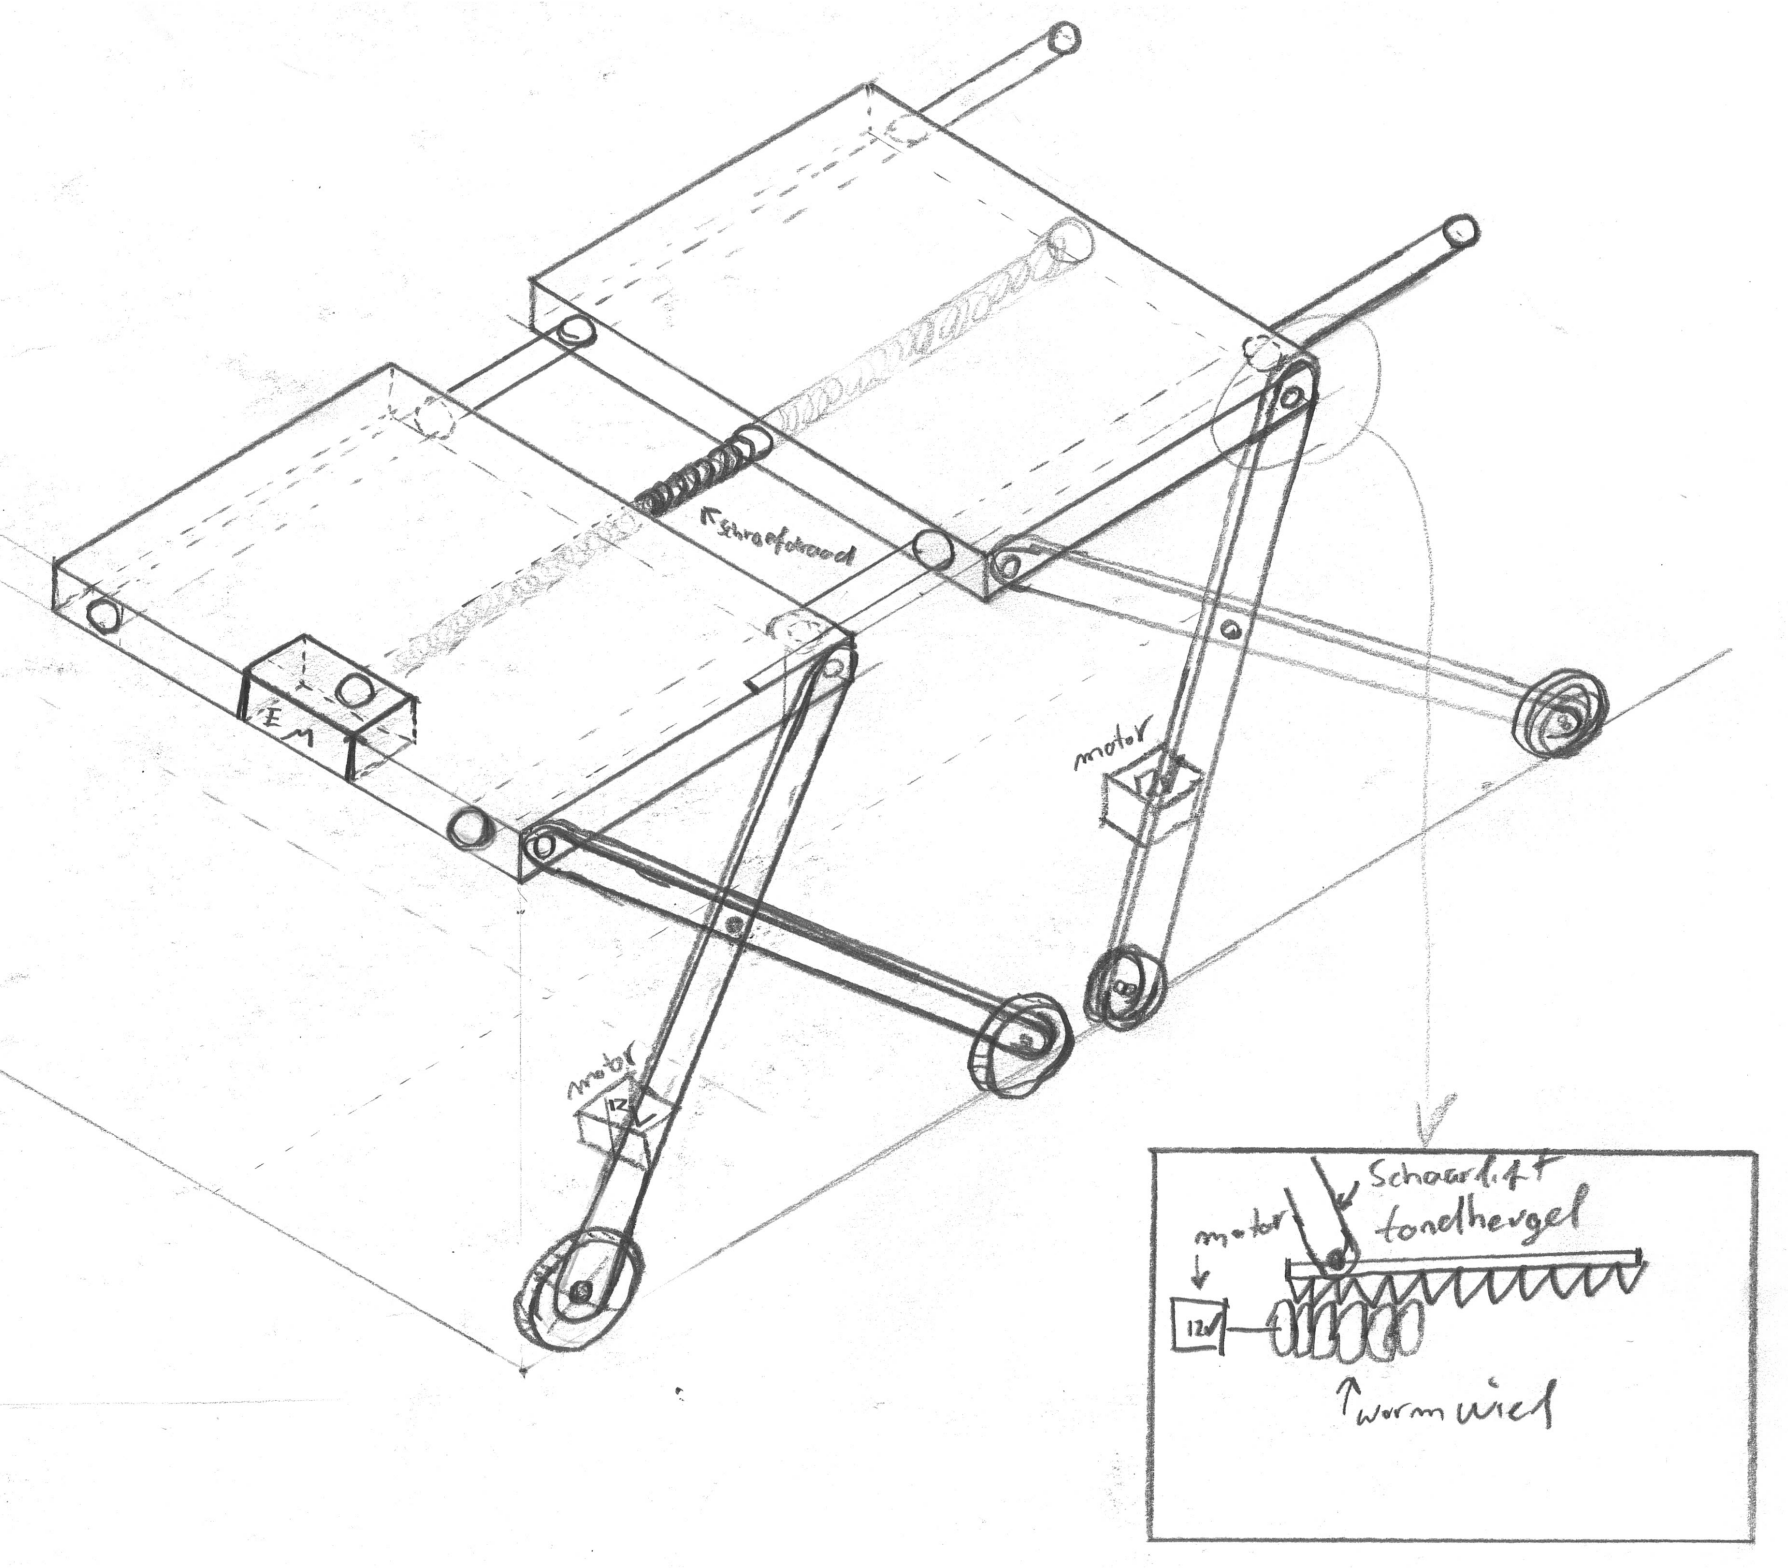
\includegraphics[width=80mm]{04_idee_ontwikkeling/isom_uitschuiver.png}
    \caption{Concept 2, de uitschuiver}
    \label{fig:isom_uitschuiver2}
\end{figure}

Het derde concept is de Inklapper. Zoals de naam al verraad klappen de pootjes en de schaarlift een voor een in waardoor de Inklapper over het obstakel heen kan rijden zonder het obstakel ook echt aan te raken, zie \cref{fig:inklapper2} en \cref{fig:inklapper_schuif2}. Bij dit concept kan het pakketje ook heen en weer worden geschoven om het zwaartepunt te veranderen. Het voordeel hiervan is dat het makkelijker te maken is met dezelfde voordelen als de Uitschuiver. Een nadeel is dat de wielen relatief veel bewegingsvrijheid hebben. 

\begin{figure}[H]
    \centering
    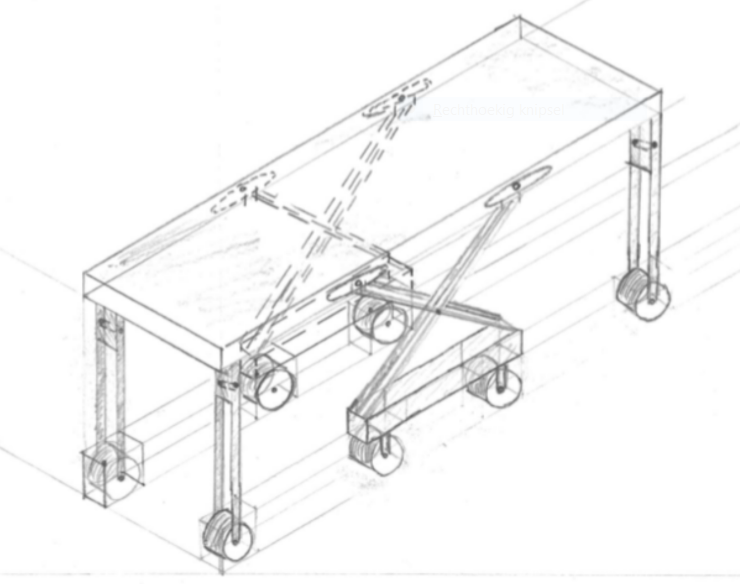
\includegraphics[width = 80mm]{Foto_inklapper.PNG}
    \caption{Concept 3, De inklapper, het in klapmechanisme}
    \label{fig:inklapper2}
\end{figure}

\begin{figure}[H]
    \centering
    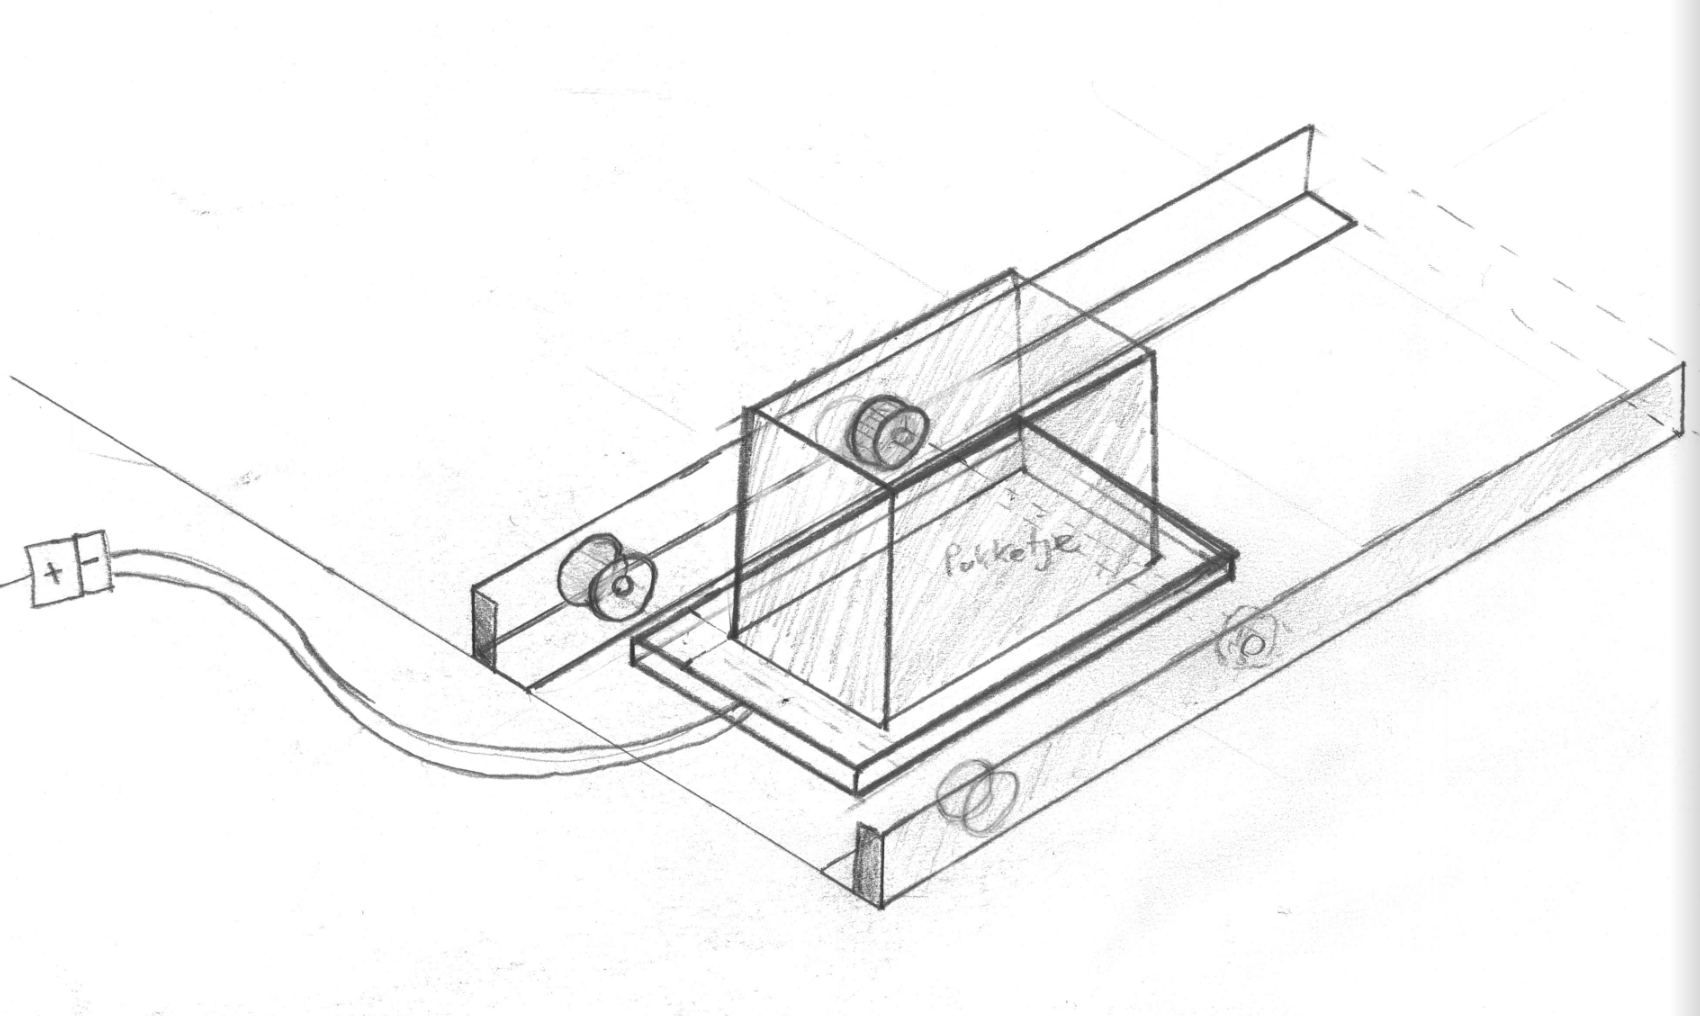
\includegraphics[width = 80mm]{04_idee_ontwikkeling/detail_uitschuiver.png}
    \caption{Concept 3, De inklapper, het schuifmechanisme}
    \label{fig:inklapper_schuif2}
\end{figure}

Het vierde concept is de Vierpoter, de Vierpoter heeft 4 poten en heeft geen variabel zwaartepunt, waardoor er met genoeg afstand tussen de wielen over het obstakel heen kan worden gestapt. De assen die aan de bovenkant te zien zijn in \cref{fig:vierpoter_totaal2} zijn er om het pakketje te ontvangen Het nadeel van de grote afstand tussen de wielen is dat het gehele ontwerp 3 keer zo lang moet worden als het obstakel en zou het in 3 delen demonteerbaar moeten zijn om te voldoen aan de eisen van de ontwerpopdracht. Het voordeel is dat het zwaartepunt niet hoeft te worden verplaatst en daardoor is het een makkelijk ontwerp om te maken.

\begin{figure}[h]
    \centering
    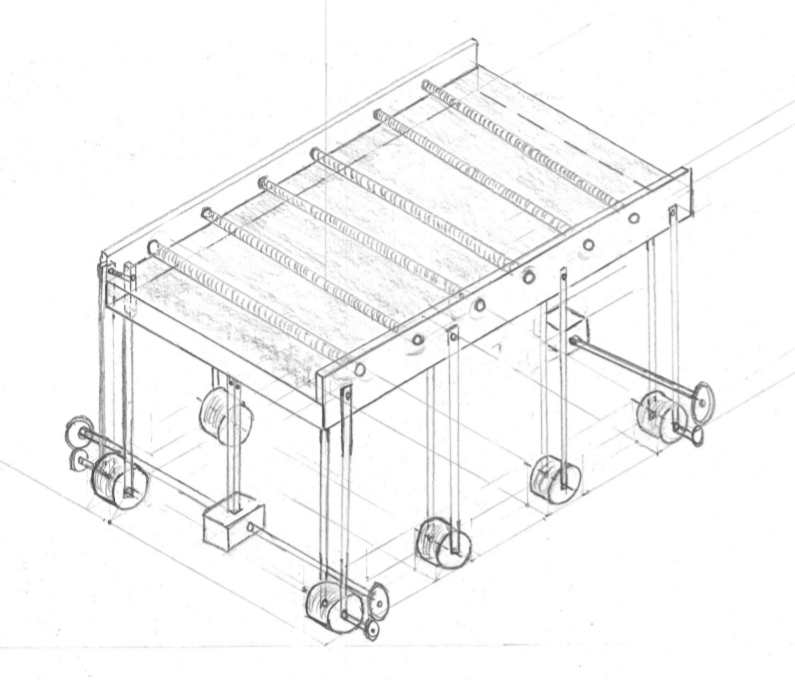
\includegraphics[width = 80mm]{04_idee_ontwikkeling/Foto_vierpoter.PNG}
    \caption{Concept 4, de vierpoter}
    \label{fig:vierpoter_totaal2}
\end{figure}
\vspace{\baselineskip}
Met de gewogen criteria methode is er uiteindelijk gekozen voor een combinatie van de Inklapper met de Vierpoter, genaamd de 'Driepoot'. De Driepoot neemt de hindernisbaan op dezelfde manier als de Vierpoter, maar heeft schaarliften onderin i.p.v. inklapbare poten. Het gebruik van schaarliften heeft twee voordelen: het is gemakkelijker te maken en het is stabieler. Het gewicht van de driepoot is 10 kg in totaal. In \cref{fig:uiteindelijke_concept} is het totaalconcept afgebeeld.

\begin{figure}[h]
    \centering
    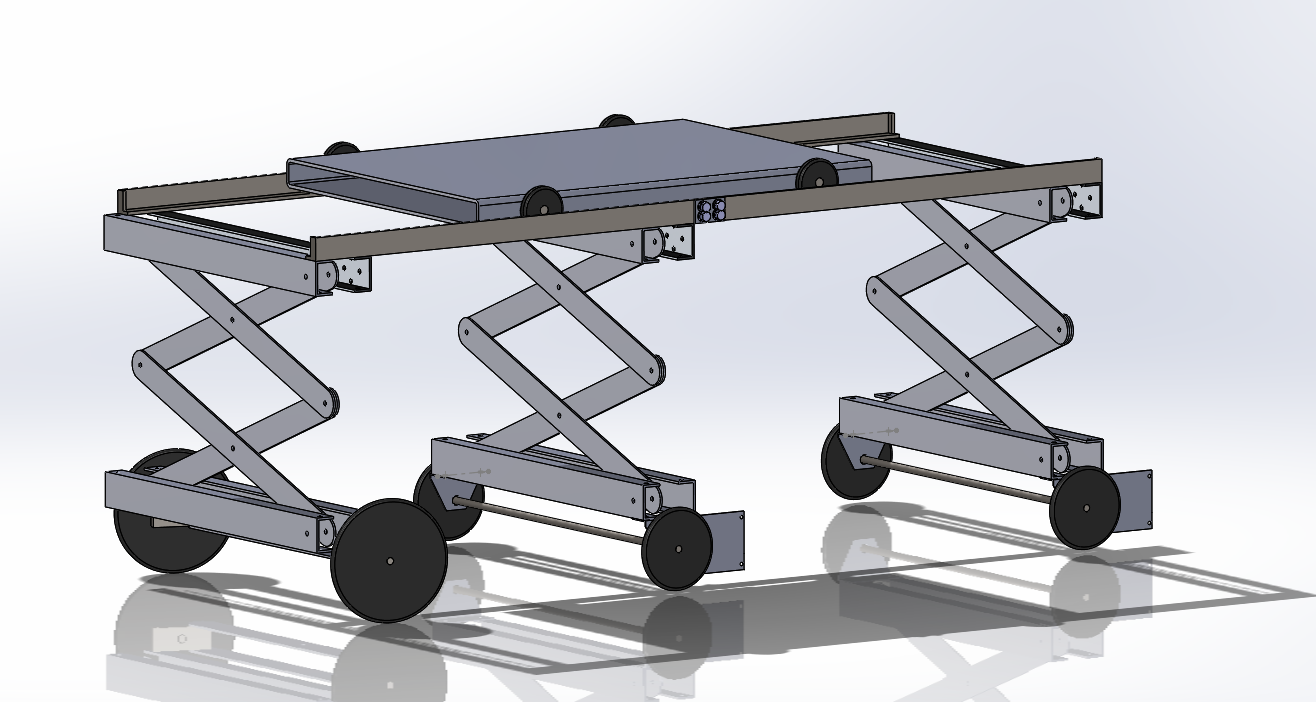
\includegraphics[width = 100mm]{04_gekozenconcept/eindconcept.png}
    \caption{Gekozen concept, inklapper (uitgewerkt)}
    \label{fig:uiteindelijke_concept}
\end{figure}

\renewcommand{\contentsname}{Inhoudsopgave}
\tableofcontents

\mainmatter
\thumbtrue

%%Zet hier je hoofdstukken neer

\chapter{Inleiding}
\label{cha:inleiding}
In 2018 is het globale pakketvolume met 16\% gestegen, van 74,7 miljard naar 87 miljard pakketjes (\cite{pitney_bowes_2018}) Men verwacht dat het aantal pakketjes 100 miljard zal bereiken aan het eind van 2020. De groei in deze markt zorgt voor een toenemende werklast van de bezorgers. Zij hebben ook een hoger risico op schouder- en rugpijn dan werknemers in andere branches. (\cite{hurley_marshall_hogan_wells_2012}). Het implementeren van een 'pakkethondje' kan helpen om zulke medische klachten te voorkomen. Eerstejaars werktuigbouwkundestudenten aan de TU Delft hebben de uitdaging gekregen om zo'n pakkethondje te ontwerpen en ontwikkelen (\cite{beek_2020_opdracht}).
\vspace{\baselineskip}

Het doel van dit rapport is het ontwerpproces van het pakkethondje in kaart te brengen en een voorspelling van de prestatie te maken. De opdracht die door TU Delft is samengesteld luidt: “De uitdaging is om een “pakkethondje” te ontwerpen dat een pakket met een gewicht van iets minder dan 10kg foutloos over een hindernisbaan weet te transporteren.” (\cite{beek_2020_opdracht}). Tijdens het ontwerpproces is er specifiek rekening gehouden met de wens dat het pakkethondje afstandbestuurbaar is. Het project kan worden opgedeeld in drie fases: het ontwerpproces, de vervaardiging en de prestatie test.
\vspace{\baselineskip}

De opbouw van dit rapport is als volgt: in \cref{cha:opdrachtanalyse} word de opdrachtanalyse, hierbij is rekening gehouden met de prestatiecriteria om een goed geïnformeerd programma van eisen op te stellen. Aan de hand van het PvE zijn er deeloplossingen en spuugmodellen gemaakt die zijn uitgewerkt tot totaaloplossingen wat in \cref{cha:ideeOntwikkeling} wordt uitgewerkt. De evaluatie van de totaaloplossingen wordt in \cref{cha:Concept_keuze} behandeld, met de evaluatie is er een keuze gemaakt voor het eindontwerp op basis van de vastgestelde prestatiecriteria. In \cref{cha:gekozenConcept} wordt het eindontwerp volledig tot detail uitgewerkt met de faal- en prestatieanalyse. Vervolgens wordt in \cref{cha:gekozenConcept} een conclusie geschreven op het ontwerpproces. 


\chapter{Opdrachtanalyse}
\label{cha:opdrachtanalyse}


\textit{In dit hoofdstuk wordt de ontwerpuitdaging geanalyseerd. Hierdoor wordt duidelijk wat er exact verwacht wordt van het eindontwerp en hoe dit gerealiseerd kan worden. De ontwerpuitdagingen worden in  \cref{se:Ontwerp_uitdagingen} opgesteld. In \cref{se:functieanalyse} is de functieanalyse te vinden. De ingewonnen informatie is te vinden in \cref{se:Ingewonnen_informatie} en \cref{cha:bijlage_C}. Het programma van eisen is te vinden in \cref{se:PVE}. In \cref{se:PC} zijn de prestatie criteria te vinden.}

\section{Ontwerp uitdagingen}
\label{se:Ontwerp_uitdagingen}
De ontwerpuitdagingen van het pakkethondje zijn:

\begin{enumerate}
    \item Er moet een betrouwbare aandrijving en energiebron gekozen worden.
    \item Er moet een mechanisme ontworpen worden voor het nemen van de hindernissen op het parcours.
    \item Er moet een manier bedacht worden om het pakket te ontvangen en af te leveren.
    \item Er moet een manier gevonden worden om het pakket te vervoeren, zonder dat het van het pakket hondje valt.
    \item Het complete Pakket hondje moet te produceren zijn in vijf werkplaats momenten van vier uur, passend binnen een budget van €200/€250.
\end{enumerate}



\section{Functieanalyse}
\label{se:functieanalyse}
De functies van het pakket hondje kan ingedeeld worden in hoofd en deelfuncties.\\
\vspace{\baselineskip}

De hoofdfuncties van het hondje zijn:
\begin{enumerate}
    \item Het mechanisme moet een lading van 10kg van A naar B kunnen verplaatsen.
    \item Het mechanisme moet over twee obstakels kunnen bewegen.
\end{enumerate}
\vspace{\baselineskip}
De deelfuncties van het hondje zijn:
\begin{enumerate}
    \item Het pakket hondje moet een interne energie bron hebben die de aandrijving verzorgt.
    \item Het pakket hondje moet een stuurmechanisme hebben.
    \item Het pakket hondje moet bestuurbaar kunnen zijn.
    \item Het pakket hondje moet het pakket ontvangen op een gewenste hoogte.
    \item Het pakket hondje moet in staat zijn om gedurende de hindernis baan het pakketje bij zich te houden.
    \item Het pakket hondje moet in staat zijn om te kunnen remmen wanner dat gewenst is.
    \item Het pakket hondje moet in staat zijn om voort te kunnen bewegen.
\end{enumerate}


\section{Ingewonnen informatie}
\label{se:Ingewonnen_informatie}
Voor het begin van het ontwerp proces is het van belang om zoveel mogelijk informatie in te winnen dat een breder beeld geeft over de mogelijke opties voor de ontwerpopdracht. De ingewonnen informatie is te zien in \cref{cha:bijlage_C}. Hieronder wordt een korte samenvatting gegeven over de onderwerpen die zijn onderzocht en welke conclusie daaruit is getrokken:\\

\begin{itemize}
    \item Mogelijke kosten
    \item Bestaande mechanismes die dezelfde functie verrichten.
    \item Mogelijke stuur mechanismes
\end{itemize}
\vspace{\baselineskip}

\textbf{Mogelijke kosten.} Uit het onderzoek naar prijzen van onderdelen is gebleken dat elektra een grote kostenpost is. Dit heeft te maken met de relatief dure prijs van elektromotoren en accu's, (\cite{123accu.nl} en \cite{Conrad}).
\vspace{\baselineskip}

\textbf{Bestaande mechanismes die dezelfde functie verrichten.} Een mogelijk interessante machine is een mars lander ( \cite{r.g._bonitz_nguyen_kim_bonitz_folkner_golombek_olson_spohn_grott_et_al._1970}).
\vspace{\baselineskip}

\textbf{Mogelijke stuur mechanismes.} Bij het onderzoek naar stuur mechanismes naast de al bekende manieren van sturen, zoals een fiets, ook alternatieve manieren onderzocht, zie \cite{Stuurmechanisme}.
\vspace{\baselineskip}


\vspace{\baselineskip}

\section{Programma van eisen}
\label{se:PVE}

De belangrijkste functionele eisen van de ontwerpopdracht zijn: 
\begin{enumerate}
    \item Het pakket hondje mag tijdens het parcours niet zijn stabiliteit verliezen of omvallen.
    \item Het pakket hondje moet zodanig bestuurd kunnen worden dat het kan worden aangedreven, afgeremd en kan sturen.
    \item Het pakket hondje moet in (eventueel gedemonteerd) in een verhuisdoos passen van $ 0,48 \times 0,32 \times 0,33 m.$
    \item Het mechanisme moet niet bezwijken bij een toegevoegde belasting van 10 kg 
    \item Bij de constructie van het pakket hondje mogen alleen frame onderdelen gelast worden.
    \item Het pakket hondje moet zijn eigen energiebron vervoeren.
    \item Het pakket hondje moet conform de CE-norm zijn.
    \item Het pakket hondje mag tijdens het parcours het pakket niet verliezen.
    \item Het pakket hondje moet in maximaal 10 minuten de hindernisbaan afleggen.
    \item De trekkracht aan het geleidende koord moet op elk moment minder dan 25 newton zijn.
\end{enumerate} 
\vspace{\baselineskip}

\section{Prestatie criteria}
\label{se:PC}

De prestatie criteria van het pakket hondje zijn:
\begin{enumerate}
    \item Het pakket hondje moet een zo moeilijk mogelijk obstakel kunnen nemen.
    \item Het pakket hondje moet zo goed mogelijk statisch en dynamisch te analyseren zijn.
    \item Het pakket hondje moet zo goedkoop mogelijk zijn.
    \item Het ontwerp moet zo min mogelijk gelaste onderdelen en zo veel mogelijk makkelijk vervangbare onderdelen bevatten (duurzaamheid).
    \item Het pakket hondje moet makkelijk te construeren en assembleren zijn.
    \item Het pakket hondje moet zo licht mogelijk zijn.
    \item Het pakket hondje moet zo min mogelijk bewegende onderdelen bevatten.
    \item Het pakket hondje moet zo snel mogelijk zijn.
    \item Het pakket hondje moet zo wendbaar mogelijk zijn.
\end{enumerate}



\chapter{Idee ontwikkeling}
\label{cha:ideeOntwikkeling}
\textit{In dit hoofdstuk is de opzet gemaakt voor het maken van het meubel hondje. Hier zijn verschillende ontwerp methodes toegepast (\cref{se:creatief_proces}), deel concepten (\cref{se:Deelontwerpen}), spuug modellen (\cref{se:Spuugmodellen}) en ook drie kansrijke totaalconcepten (\cref{se:totaalconcepten}).}


\section{Creatief proces}
\label{se:creatief_proces}
{\bf In de eerste weken zijn er brainstormsessies gehouden om oplossingen te vinden op de deelfuncties.}
\subsection{ACCREx}
Tijdens het ontwerpproces is er gebruik gemaakt van diverse methodes voor het bedenken van ideeën. Ook is er gebruik gemaakt van ACCREx, (\cite{coelho_2011}), hier is voor gekozen omdat hier een aantal interessante mogelijkheden lagen voor het toepassen van ACCREx.\\
Bij deze ontwerpopdracht was het van belang om een oplossing te bedenken om over het talud te komen. Daarom is er voor gekozen om bij dit ontwerp probleem ACCREx toe te passen. ACCREx is toegepast door 2 manieren van voortbewegen tegen elkaar uit te zetten en te kijken of er daar ideeën uit kunnen worden gehaald. Er is gekozen om horizontale verplaatsing tegen verticale verplaatsing uit te zetten. Deze combinatie van manieren gaf een frame waarin ideeën konden worden bedacht. \\

\subsection{Bio inspired design}
Tijdens het ontwerp proces is er ook gekeken naar alternatieve vormen van ideeën en oplossingen generen, zoals bio-inspired design. De opgave was een paar voorbeelden van de natuur te bedenken die het zelfde probleem heeft moeten over overwinnen.
\vspace{\baselineskip}

\textbf{Duizendpoot.} Na onderzoek kwam al snel een duizendpoot naar voren. Het interessante van een duizend poot verraad de naam al, de hoeveelheid pootjes. Wanneer er een groot aantal pootjes wordt toevoegt in een mechanisme is het in staat om voort te bewegen op een manier waarbij het lijkt alsof het rolt. Het probleem van een lopend mechanisme is dat het moeilijk is om het pakketje recht te houden. Dit wordt opgelost door middel van veel pootjes, daarom is de duizendpoot interessant in dit onderzoek. Ook blijft de duizendpoot overeind als niet alle poten zich op de grond bevinden. Dit principe kunnen we goed gebruiken voor ons concept.\\

\vspace{\baselineskip}
{\bf Kruiper.} De rups was een voorbeeld dat al snel naar boven kwam. De rups maakt gebruik van het feit dat hij zijn lichaam kan intrekken en kan uitrekken. Door zich vast te klemmen met het voorste gedeelte van zijn lichaam kan hij het achterste deel naar zich toe trekken als het ware. Om zich dan voort te bewegen zet hij zijn achterkant vast en drukt als het ware zijn lichaam naar voren, hij rekt zich dan uit.
\vspace{\baselineskip}
\\
{\bf Hopper.} Ook de sprinkhaan en de haas kwamen na verder onderzoek naar voren. Deze twee organismes maken gebruik van hun krachtige achterpoten om niet te lopen maar te springen als het ware. Relatief kleine obstakels zijn voor deze wezens geen probleem omdat zij er gewoon over heen springen. Dit zou wellicht kunnen toe worden gepast in het ontwerp project.
\vspace{\baselineskip}
\\
{\bf Mantis car.} Het laatste idee wat werd gegenereerd door de groep was een 'mantis-car'. Dit concept is gebaseerd op hoe een sprinkhaan zijn poten gebruikt om zijn prooi vast te grijpen. Ook is de vorm van de poten cruciaal geweest voor het concept. Het principe 'mantis-car' is eigenlijk het vastklemmen met mechanische poten op het obstakel en de rest van het voertuig zich hierdoor omhoog te hijsen.\\
\vspace{\baselineskip}

\subsection{Morfologische kaart}
Door op verschillende manieren te brainstormen zijn er diverse oplossingen voor elke deel functie gevonden. Deze zijn samengebracht in een morfologische kaart (\cite{toolbox_voor_ontwerpers_ipo_windesheim}). Deze kan worden gevonden in \cref{ap:bijlage_A}. \\


\section{Deel ontwerpen}
\label{se:Deelontwerpen}
Om tot kansrijke concepten te komen, heeft elk groepslid een combinatie van oplossingen uit de morfologische kaart (zie \cref{ap:bijlage_A}) uitgewerkt tot een totaaloplossing. Het doel hier van is om concreter na te denken over hoe deeloplossingen samen kunnen werken. Zo kunnen zwakke plekken in elk ontwerp later als spuugmodel uitgewerkt worden en in het uiteindelijke ontwerp geïntegreerd worden.\\
\vspace{\baselineskip}

{\bf Schuiver.}
De schuiver maakt gebruikt van twee schaarliften en een uitschuif systeem. Aan de twee schaarliften zijn wielen verbonden die worden aangedreven, hiermee kan het systeem zichzelf voortbewegen. De schaarliften hebben twee functies, ten eerste zorgen ze ervoor dat het hoogteverschil van het pakketje kan worden bereikt. De tweede functie van de schaarliften is het overbruggen van de obstakel. Als één schaarlift opklapt terwijl de ander open blijft, kan de wagen met een stappende beweging over het obstakel heen 'lopen'. \\

\vspace{\baselineskip}
{\bf Inklapper.}
De inklapper is gebaseerd op het principe van inklapbare pootjes. Het ontwerp heeft 4 paar pootjes die allemaal in het verlengde van zichzelf kunnen inklappen. De inklapper is aangedreven door een verbrandingsmotor. De vier wielen aan de linkerkant zijn onafhankelijk van de vier wielen aan de rechter kant aangedreven. Dit zorgt ervoor dat hij zichzelf kan sturen door een kant van de wielen te laten rijden en de andere kant te laten remmen. De inklapper neemt het talud door zijn pootjes erop te laten botsen en dat ze dan inklappen. als de pootjes er weer over zijn klappen ze weer uit. Dit gebeurt met alle vier de paren zodat het mechanisme erover heen kan komen zonder het pakket te laten kantelen. Zie voor meer informatie \cref{fig:inklapper_tekening}. \\

\begin{figure}[H]
    \centering
    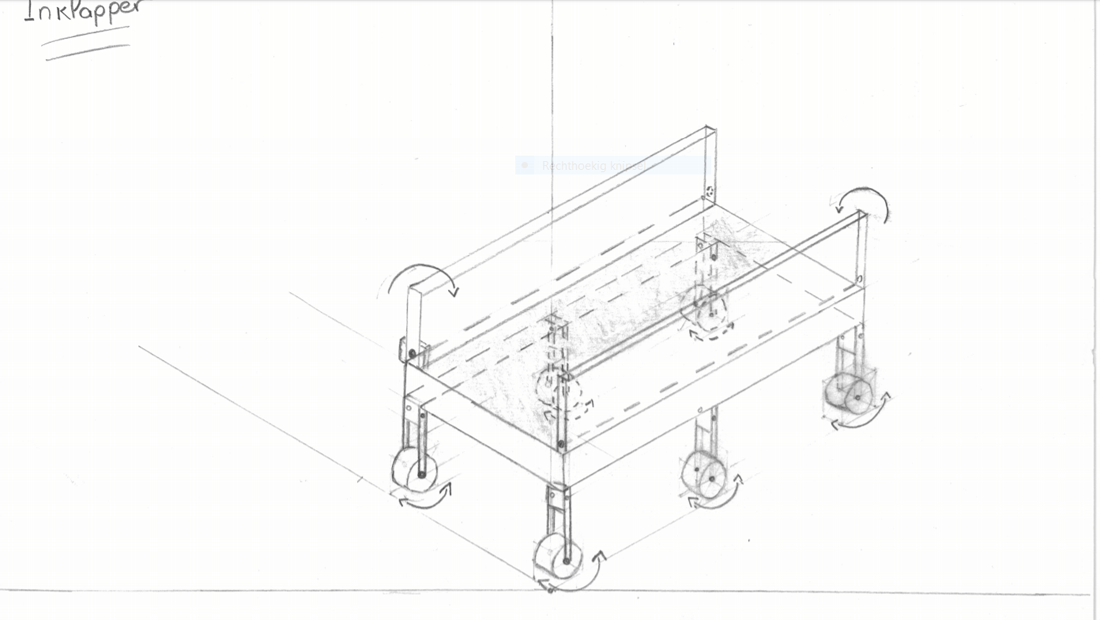
\includegraphics[width = 100mm]{04_idee_ontwikkeling/Inklapper,_deelontwerp_Beer.PNG}
    \caption{Tekening van het deelconcept inklapper.}
    \label{fig:inklapper_tekening}
\end{figure}

\vspace{\baselineskip}
{\bf Fietskar}. Dit concept maakt gebruik van een schaarlift dat het systeem omhoog brengt. Hierdoor hebben de voorste en achterste wielen geen contact meer met de grond. Vervolgens rijdt het karretje zijn voorste wiel over het talud. Eenmaal met zijn voorste wiel over het talud trekt hij zijn schaarlift in rijdt hij zijn schaarlift er overheen. Deze beweging wordt herhaald om de achterste wielen over het talud te krijgen. Het sturen doet hij met een fietswiel mechanisme wat aangedreven wordt door een fietsstuur. De fietsstuur wordt aangedreven met een servomotor die op afstand kan worden bestuurd Voor meer informatie zie \cref{fig: fietscar}.

\begin{figure}[H]
    \centering
    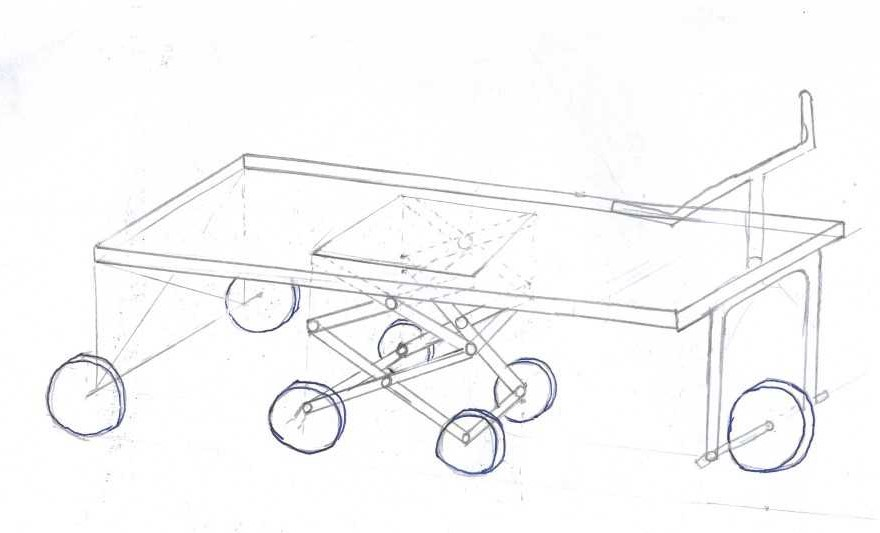
\includegraphics[width = 80mm]{04_idee_ontwikkeling/Deelontwerp-Kevin.jpeg}
    \caption{Tekening van deelconcept fietscar}
    \label{fig: fietscar}
\end{figure}

\vspace{\baselineskip}
{\bf Haaktank} De haaktank maakt gebruik van grote rupsbanden om over het talud heen te komen een een grijphaak om grotere obstakels te overwinnen. Het wordt aangedreven door elektromotoren en wordt radiografisch bestuurd. Het pakket wordt met spanbanden bevestigd zodat het stabiel blijft tijdens transport. Voor een isometrische tekening zie \cref{fig:Haaktank}.


\begin{figure}[H]
    \centering
    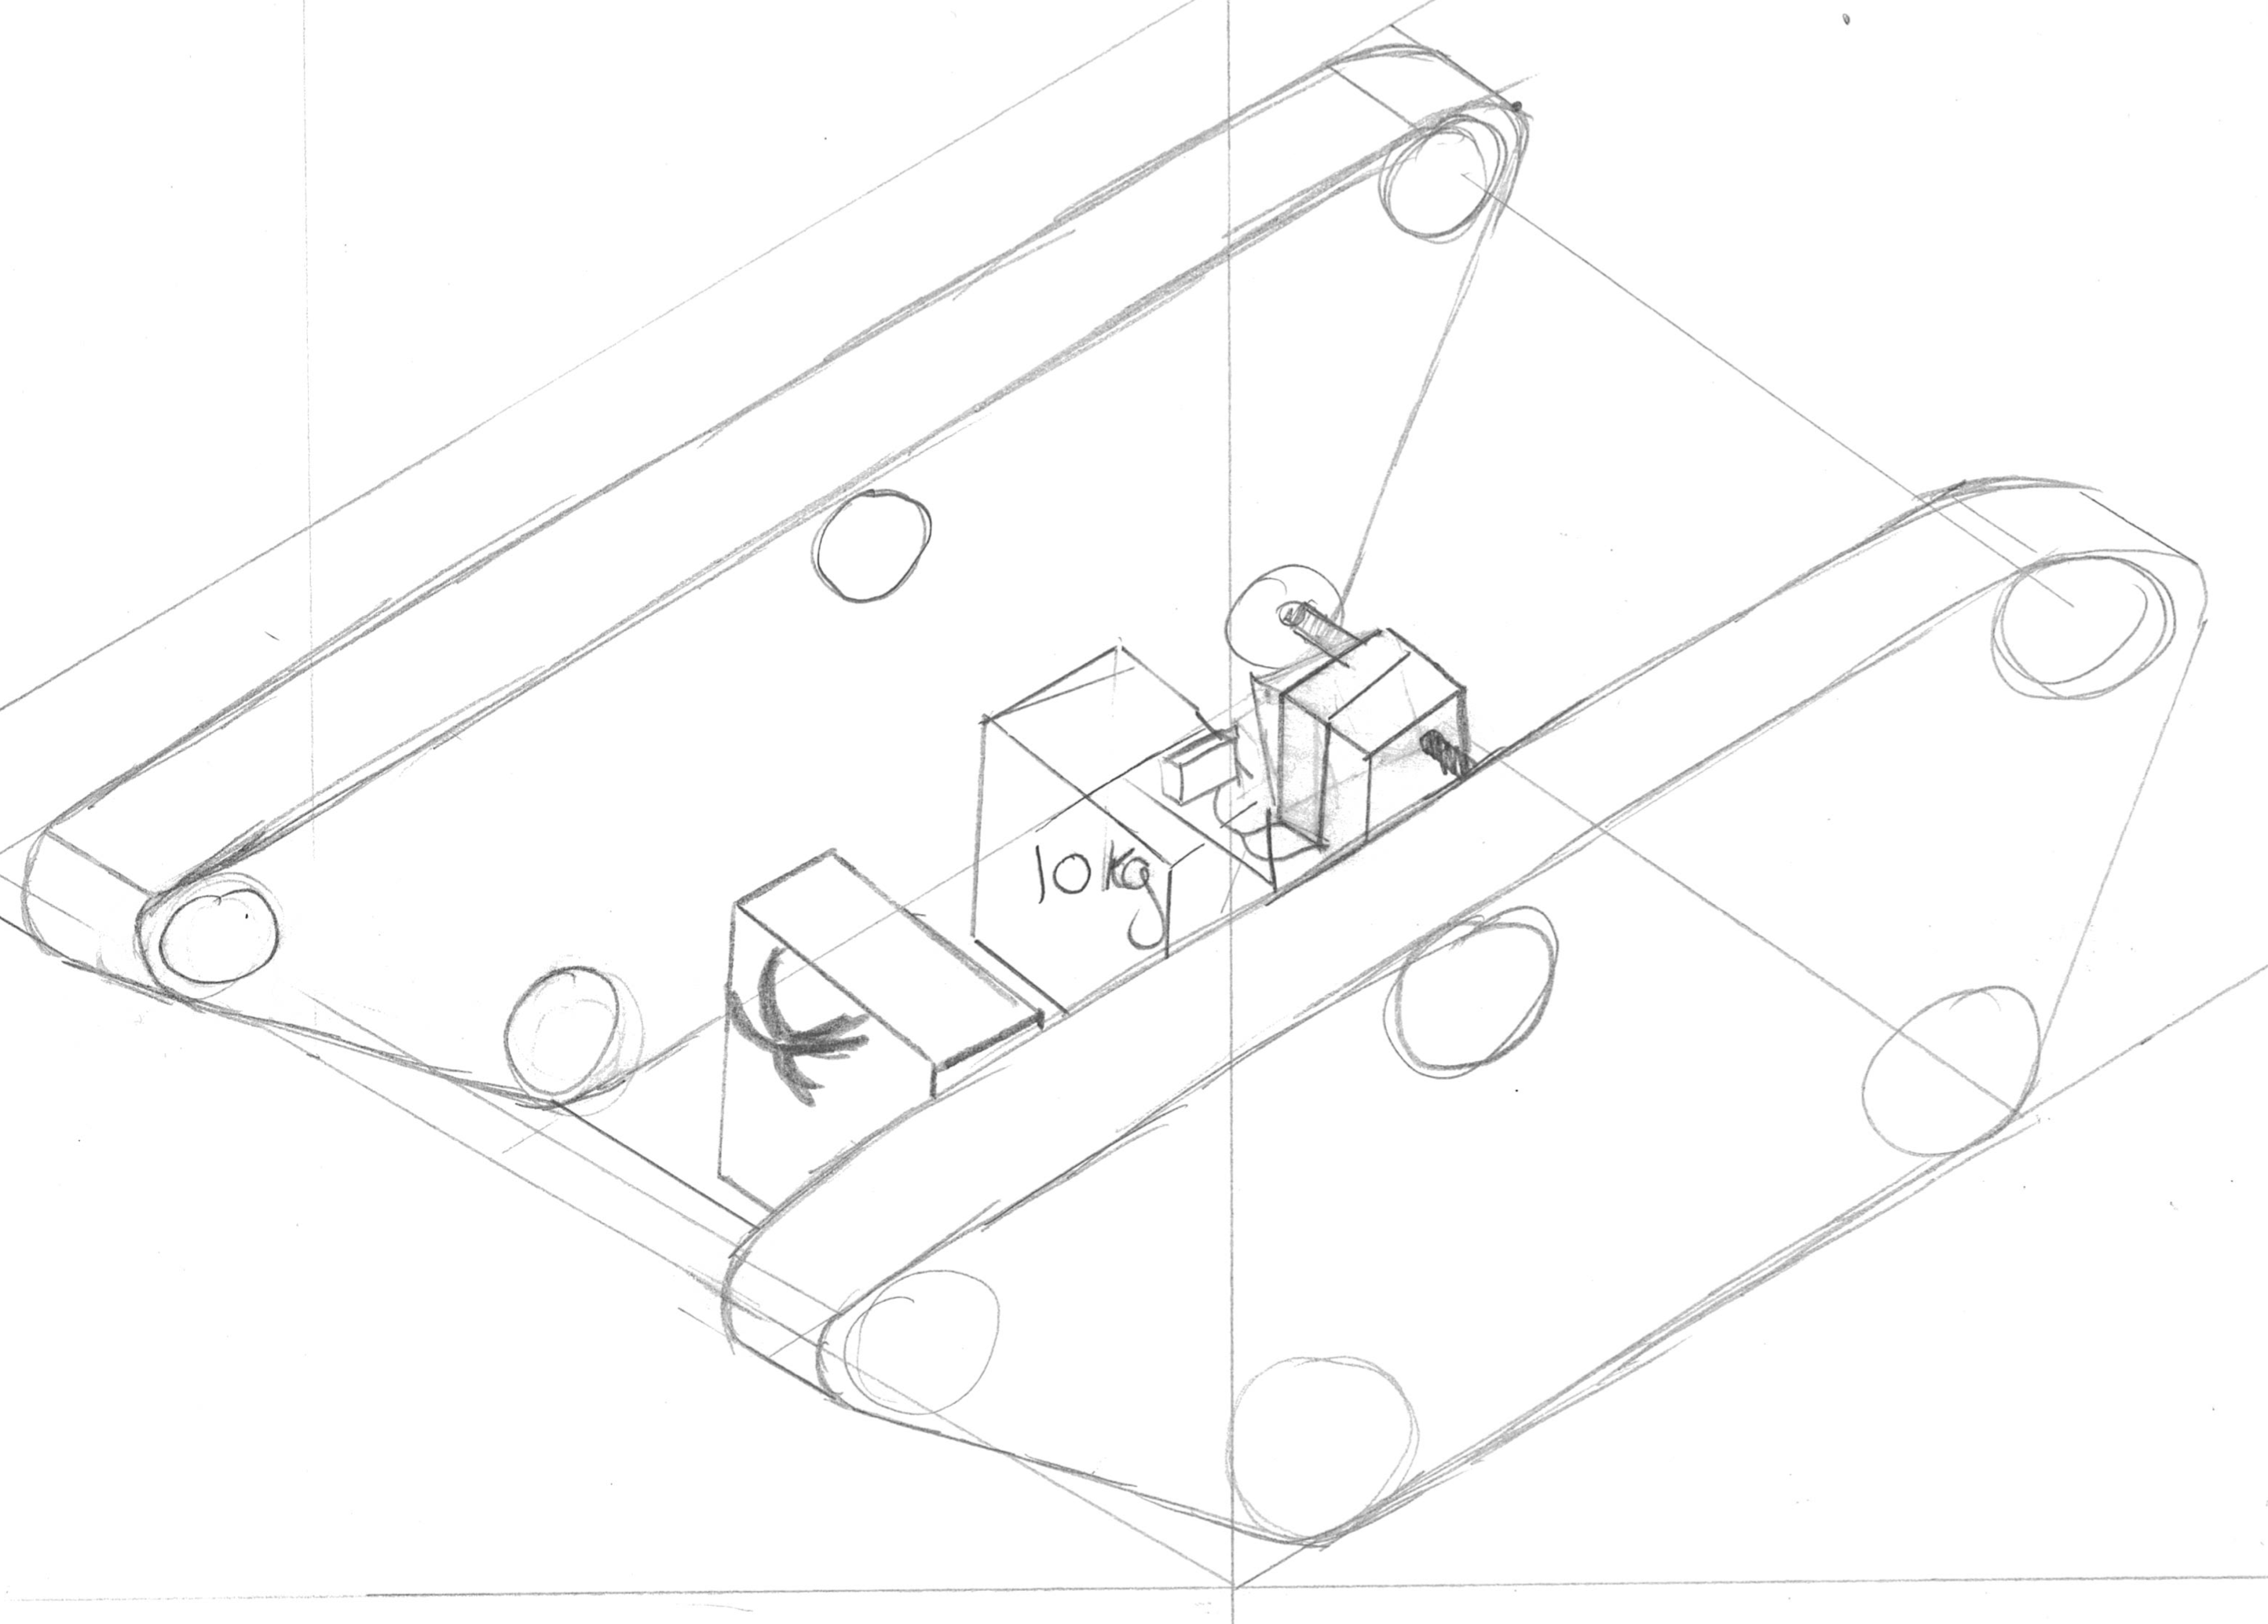
\includegraphics[width = 60mm]{04_idee_ontwikkeling/Deel_ontwerp_robin.png}
    \caption{Isometrische tekening van de Haaktank}
    \label{fig:Haaktank}
\end{figure}


    
\vspace{\baselineskip}
{\bf Strand beest.} 
Het strand beest maakt gebruik van een 4-stangen mechanisme om te lopen, hierdoor is hij in staat om over de hindernissen te stappen. Hij kan op gelijke hoogte komen met het pakketje door middel van een schaarlift. door de omsluitende wanden kan het pakketje niet vallen. Om het pakketje af te geven heeft het een klepje die open kan aan de voorkant om het pakketje er weer uit te schuiven. Hij stuurt door onafhankelijke aandrijving. De 4 stangen worden aangedreven door een elektromotor. Voor een beter beeld zie \cref{schaarlift_hilbert}.

\begin{figure}[t]
    \centering
    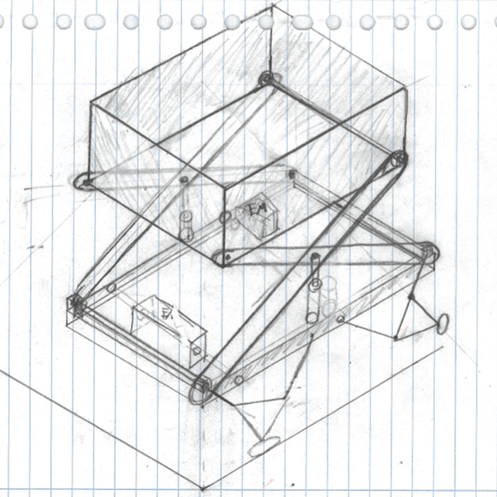
\includegraphics[width = 100mm]{04_idee_ontwikkeling/Deeloplossing_schaarlift,_Hilbert_(1).PNG}
    \caption{Tekening van deelconcept strandbeest}
    \label{schaarlift_hilbert}
\end{figure}

{\bf Mantistank}. 
De mantistank is gebaseerd op onafhankelijke aandrijving en overkomt de taluds d.m.v. de grijphaken, zie \cref{mantistank_max} Er is onafhankelijke aandrijving gerealisserd door stepper motoren. De 2 rupsbanden hebben allebei een eigen as zodat er geen differentiaal is en de onafhankelijke aandrijving gebruikt kan worden om te sturen. Het concept kan obstakels overkomen door middel van een soort grijp systeem, waarom dit concept ook wel de ‘mantis-car’ wordt genoemd, alias de mantis in de natuur. Het pakketje wordt opgevangen en ingesloten door middel van het pakket op het wagentje te schuiven, waarna er een drukplaat naar beneden wordt gedrukt waardoor de wanden insluiten door middel van trekveren. Dit laatste is alleen niet aangegeven op de tekening. \\
\vspace{\baselineskip}

\begin{figure}[H]
    \centering
    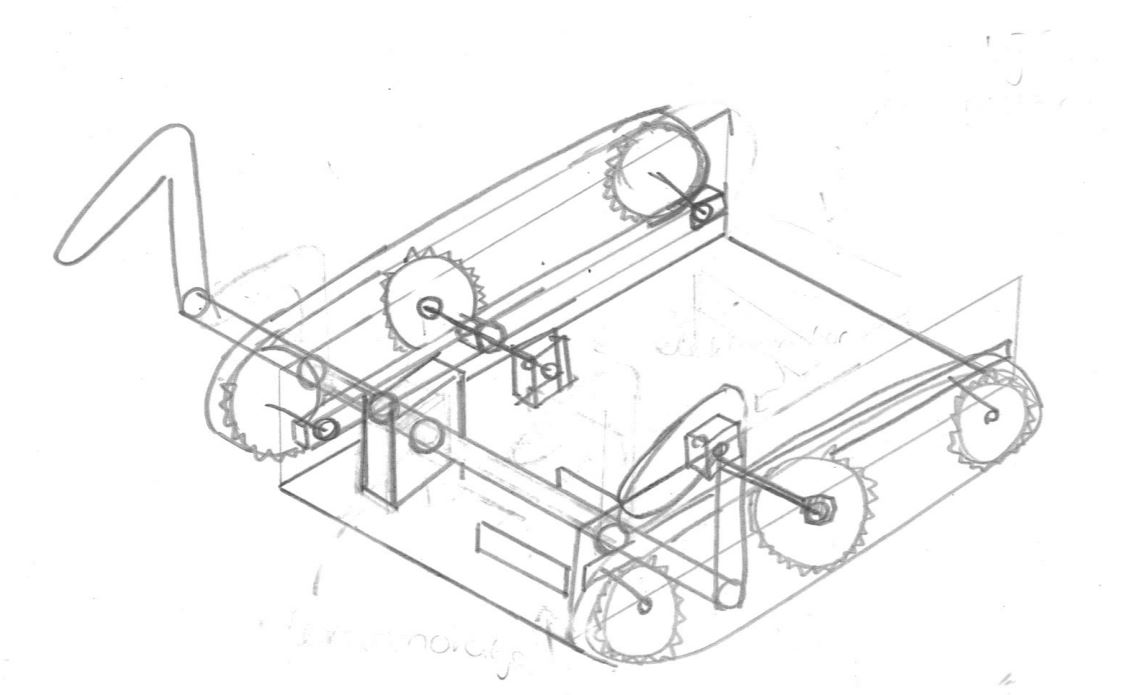
\includegraphics[width = 100mm]{04_idee_ontwikkeling/deelconcept_mantistank.JPG}
    \caption{Tekening deeloplossing mantistank}
    \label{mantistank_max}
\end{figure}

\section{Spuugmodellen}
\label{se:Spuugmodellen}
\vspace{\baselineskip}
Tijdens het ontwerpfase is het van groot belang dat er spuugmodellen worden gemaakt om beter inzicht te krijgen op de werking van de mechanismen. Vanuit de morfologische kaart zijn er een aantal spuugmodellen, waarvan de meest kansrijke vervolgens zijn uitgewerkt tot een werkelijk deeloplossing. 
\subsection{gekozen spuug modellen}
\vspace{\baselineskip}

{Om zo veel mogelijk inzicht te krijgen in de mogelijkheden om verschillende ontwerpproblemen aan te pakken is ervoor gekozen om een aantal spuugmodellen te maken.} \\

\begin{description}
\item[A.] {\bf Schaarlift.}\\ 
Het eerste gekozen spuugmodel is een model van een schaarlift. Het doel van het maken van een schaarlift was om te kijken waar eventuele veren moesten worden geplaatst en hoe de schaarlift optimaal zou werken.  Voor meer informatie zie \cref{fig:plaatje_schaarlift}.

\begin{figure}[H]
\centering

    
\includegraphics[width = 50mm, angle =270 ]{04_idee_ontwikkeling/IMG_0892.jpg}
    \caption{Spuug model schaarlift}
    \label{fig:plaatje_schaarlift}
\end{figure}

\vspace{\baselineskip}

\item[B.] {\bf Inklap wielen.}\\
Het is een interessant spuugmodel omdat het gebruik van inklapwielen een kansrijke deeloplossing is en het essentieel is om dan vroeg achter de ontwerp uitdagingen van zo 'n inklap wiel te komen. Het spuugmodel is uit lego gemaakt omdat dit makkelijk te assembleren was en er veel verschillende manieren zijn om het te maken zodat er ook kon worden gekeken naar hoe het optimaal kon worden gedaan. Voor meer informatie zie \cref{fig:inklapwielen}. \\

\begin{figure}[H]
\centering

    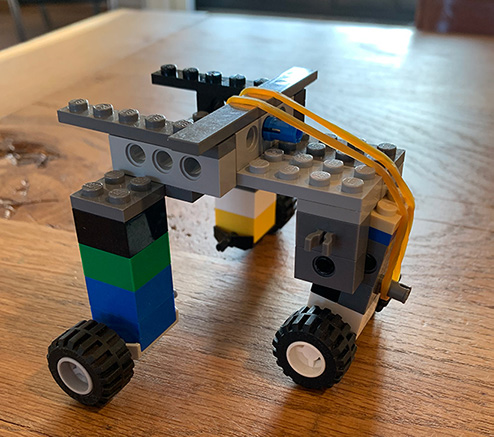
\includegraphics[width = 50mm, angle = 270]{04_idee_ontwikkeling/Inklapwielen.jpg}
    \caption{Spuug model inklapwielen}
    \label{fig:inklapwielen}
\end{figure}

\item[C.] {\bf Mantis klauwen.}\\
De mantis klauwen zijn relatief makkelijk te construeren en te assembleren op een frame. Hierdoor is het een interessant spuugmodel omdat het wellicht makkelijk is om dit spuugmodel te perfectioneren. Het leek de groep ook essentieel om te onderzoeken hoe lang de klauwen van zo'n mantis systeem moesten zijn voordat het werkte. In \cref{fig:Mantis_spuug} is een spuugmodel van de Mantis Car afgebeeld. \\

\begin{figure}[H]
\centering
    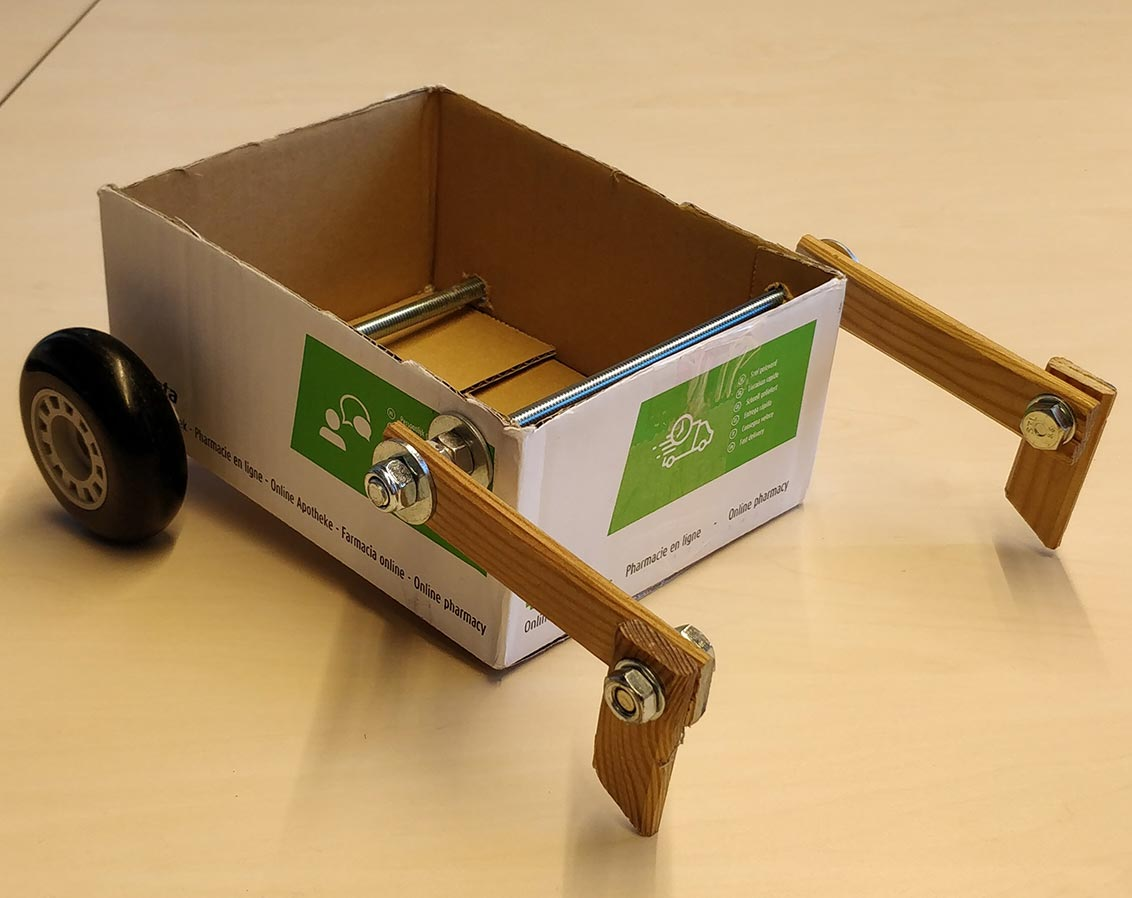
\includegraphics[width = 50mm]{04_idee_ontwikkeling/Mantis_spuugmodel.jpg}
    \caption{Spuugmodel Mantis Car}
    \label{fig:Mantis_spuug}
\end{figure} 

\item[D.] {\bf Stuursysteem.}\\
Er werd ook gekeken naar verschillende stuursystemen, wat werkt en wat niet werkt. Daarom is er gekozen voor het maken van een stuursysteem dat lijkt op het sturen van een fietswiel. Dit sturen wordt gerealiseerd door middel van een servo. (zie \cref{fig:Fietsstuur}). \\

\begin{figure}[H]
    \centering
    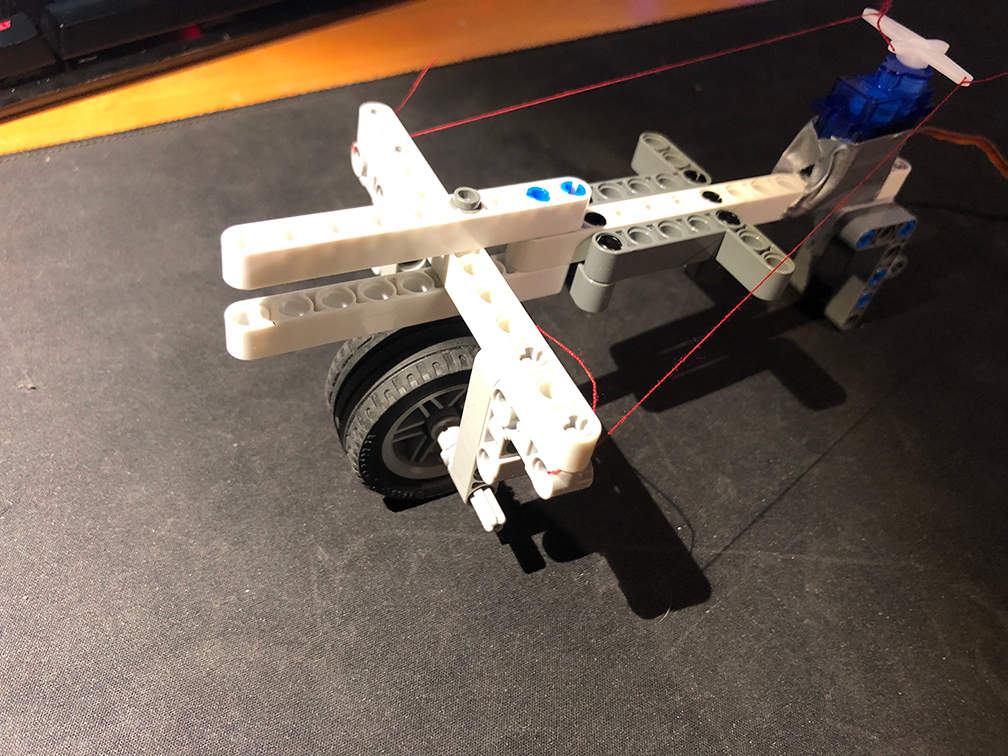
\includegraphics[width = 50mm]{04_idee_ontwikkeling/fietsstuur.jpg}
    \caption{Spuugmodel Stuurssysteem}
    \label{fig:Fietsstuur}
\end{figure} 



\item[E.] {\bf Radiografische besturing.}\\
In verschillende deel ontwerpen wordt er gebruik gemaakt van radiografische besturing. Het is belangrijk om te weten hoe deze radiografische besturing gerealiseerd kan worden voordat het toegepast wordt in een ontwerp. Radiografische besturing bleek niet moeilijk te realiseren te zijn. Zie \cref{fig:arduino}.


\begin{figure}[H]
    \centering
    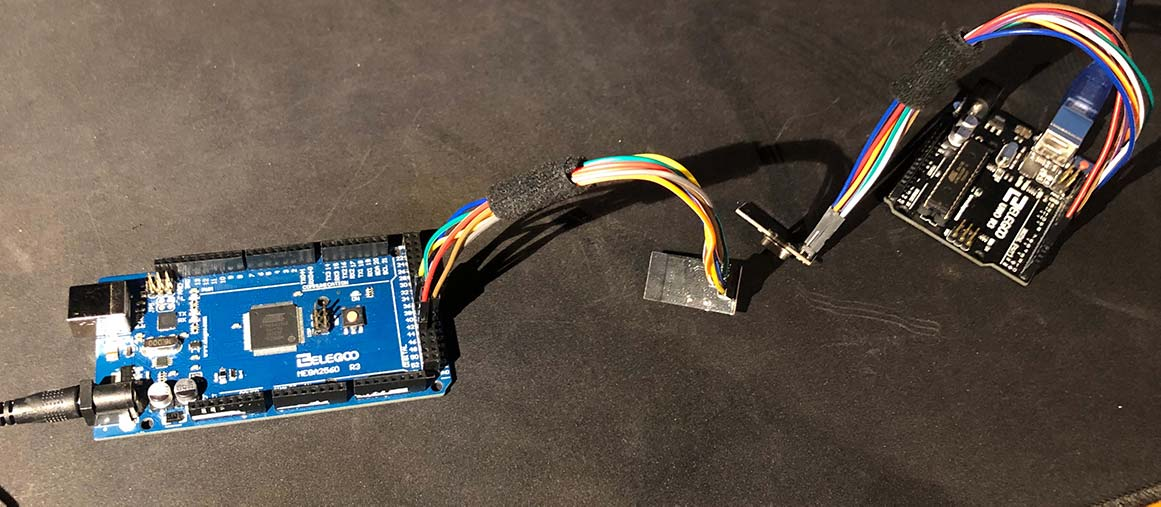
\includegraphics[width = 80mm]{04_idee_ontwikkeling/RC_arduinos.jpg}
    \caption{Arduino's communicerend over radiosignalen.}
    \label{fig:arduino}
\end{figure} 


\end{description}

%%veel plaatjes, met onderschrift dat past bij verwijzing naar foto's, (zie tekst)

\subsection{Evaluatie spuug modellen}
\vspace{\baselineskip}

\begin{description}

\item[A.] {\bf Schaarlift.}\\
De schaarlift is een relatief makkelijk principe als het gaat om fabricage en werking. Toch zijn er een aantal complicaties gevonden waar nog oplossingen voor moesten worden gevonden. \\
Een probleem van de schaarlift is de aandrijving ervan. Om de schaarlift te laten in klappen moeten de twee uiteinden van de schaarlift zich van elkaar af bewegen. Dit kan worden gerealiseerd worden door middel van een roterende as met een touwtje die zich opwindt en zo een van de uiteinden weg trekt. Dit kan ook worden opgelost door een tandheugel. Het probleem hiervan is dat ervoor gezorgd moet worden dat het tandwiel op de tandheugel moet blijven. \\
Nog een probleem van een schaarlift is de verplaatsing van de uiteinden. Doordat de uiteindes zich van elkaar af bewegen kunnen ze niet worden vastgeklemd. De uiteindes mogen een graad van vrijheid hebben, zodat ze wel horizontaal van elkaar af kunnen bewegen. \\ 

\item[B.] {\bf Inklap wielen.}\\
De inklapbare wielen was een makkelijk te maken spuug model, maar het gaf veel inzicht. \\ 
Een van de voordelen van inklapbare wielen is dat  het op veel verschillende manieren kan worden toegepast. Het is namelijk mogelijk om de wieltjes via een mechanische aandrijving in te laten klappen en uit te laten klappen. Dit zorgt ervoor dat het pakket hondje in principe het talud niet aan hoeft te raken. Het voordeel hiervan is dat het pakket hondje allerlei soorten obstakels kan nemen.\\
Ook kan ervoor worden gekozen dat het pakket hondje als het ware tegen het talud aanrijd en dat de voorste pootjes, die het talud raken, door de voortbeweging van het pakket hondje worden ingeklapt. Als dit bij alle pootjes wordt toepast en als er een veer wordt bevestigd die de pootjes terug laten klappen, kan het pakket hondje er zo gemakkelijk over heen. \\
Een nadeel van de inklapbare wielen zijn dat er een lock-systeem moet worden bedacht zodat de pootjes niet onder hun eigen gewicht inklappen. Hiervoor zijn oplossingen te bedenken, maar dit moet dan elektrisch worden aangedreven en hoe meer dingen er moeten worden bestuurd, hoe moeilijker het wordt.\\

\item[C.] {\bf Mantis klauwen.}\\
Het systeem van de mantis klauwen is gebaseerd op de armen van een sprinkhaan. Dit mechanisme zorgt voor een klimmende werking waardoor het pakkethondje over obstakels kan rijden. Om de klauwen te realiseren worden er twee armen bevestigd aan een as. Vervolgens wordt de as aangedreven, dit zorgt ervoor dat de armen een cirkelbeweging maken. Als het pakkethondje een obstakel tegenkomt zullen de armen het hondje omhoogtrekken. De voorwaartse aandrijving van de wielen gecombineerd met de klimmende beweging van de mantis klauwen zorgt ervoor dat het pakkethondje over het obstakel komt. 

\item[D.] {\bf Stuursysteem.}\\
Het stuursysteem is een essentieel onderdeel van het pakket hondje en daarom is het belangrijk om er over na te denken en er ook een spuug model van te maken.\\
Er is gekozen voor een aandrijving met een stuursysteem zoals bij een fiets dat is aangedreven door een servo. Dit systeem was kansrijk omdat het relatief makkelijk te assembleren was en het ook betrouwbaar is. Bij het maken van dit spuugmodel zijn er geen problemen gevonden, waardoor dit een realiseerbare deeloplossing is voor het stuursysteem, mits het in het ontwerp toe te passen is.\\

\item[E.] {\bf Radiografische besturing. }\\
Radiografische besturing blijkt simpel, goedkoop en betrouwbaar te zijn. De code schrijven voor de Arduino's bleek niet ingewikkeld. Ook zijn de materialen voor radiografische besturing niet duur, de enige extra materialen zijn twee zendertjes van ongeveer 2 euro per stuk. (\cite{amazon.de_RC_REMOTE}) Ook kan met de zendertjes eenvoudig de bandbreedte van de zenders in kaar gebracht worden. Hiermee kan men een bandbreedte kiezen waar nog niet veel activiteit is en kan zonder verstoring verzonden en ontvangen worden. \\
Het bereik van de zenders is ook getest, en blijkt in een open veld zonder storing meer dan 50 meter te zijn. Dit zal dus geen hinder vormen tijdens de prestatietest. Waar nog wel twijfel bestaat is of veel deelnemende groepen radiografische besturing toe zullen passen. Als dit zo is, dan kan het voorkomen dat de bandbreedte van de zenders compleet in gebruik is, of dat een andere deelnemer gaat storen in onze gekozen bandbreedte tijdens de test. Daardoor zou het voordelig zijn als er ter plekke op het testveld alsnog gekozen kan worden voor bedraadde besturing. 

\end{description}


\section{Uitgewerkte concepten}
\label{se:totaalconcepten}
%%Van alle drie de concepten mooie tekeningen en een korte uitleg


%%Verander vooral de dom klinkende namen:
\subsection{concept 1: \textit{Mantis Car}} 
\label{se:concept_1_mantis_car}

\begin{figure}[H]
    \centering
    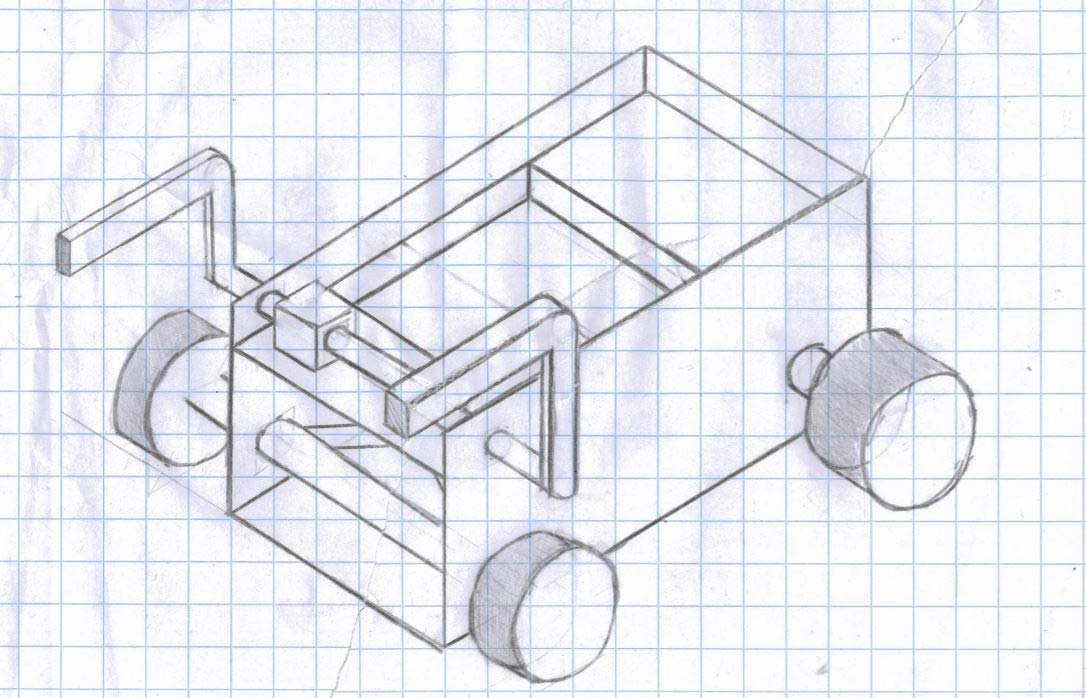
\includegraphics[width = 100mm]{04_idee_ontwikkeling/deeloplossing_mantis.JPG}
    \caption{Isometrische tekening Mantis Car}
    \label{fig:deeloplossing_mantis}
\end{figure}

De mantis car werkt door middel van grijphaken die zijn gebaseerd op de poten van een sprinkhaan, wat de naam van het concept eigenlijk al verklapt. De grijphaken worden aangedreven door een elektromotor verbonden aan de as tussen de twee grijphaken, zie \cref{fig:deeloplossing_mantis}. Deze grijphaken zouden zich kunnen vastklemmen aan het talud, en de kar zou zich op deze manier omhoog kunnen takelen.\\

Dankzij de bevindingen die zijn opgedaan tijdens het testen van het spuugmodel is er gekozen om dit concept verder uit te werken. Ten eerste bleek dat de grijphaken niet voldoende statisch gebalanceerd waren. Het omhoogbrengen van de haken vereiste een aanzienlijk moment terwijl het omlaag brengen moeiteloos ging. De motor zou dan een variabele moment moeten leveren. Om dit te voorkomen wordt een extra set haken aan de as te bevestigen, zie \cref{fig:Mantis_haak}. Dit zorgt ervoor dat de motor een minder groot moment moet leveren om de haken tot beweging te brengen en dat het moment constant blijft.
\begin{figure}[H]
    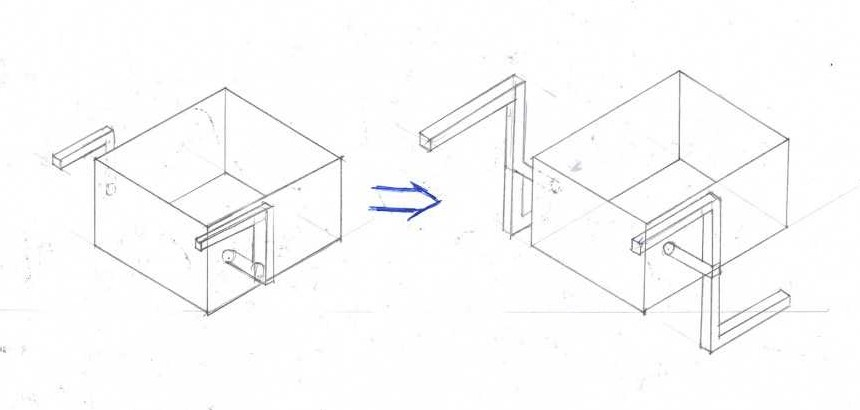
\includegraphics[width = 100mm]{04_idee_ontwikkeling/Mantiscar_armen.jpeg}
    \caption{Verbetering van de haken van de Mantis Car}
    \label{fig:Mantis_haak}
\end{figure}

\vspace{\baselineskip}
In het midden van de Mantis Car komt een schaarlift om het pakketje te ontvangen en af te leveren. De schaarlift wordt tot beweging gebracht door een stuk draadeind aan te drijven met een DC motor. Het draadeind gaat door de onderste as van de schaarlift waar een gat in is geboord van schroefdraad. Door het draadeind aan te drijven zal de schaarlift heen en weer bewegen en dus ook een verticale beweging opdoen. In \cref{fig:Schaar_boven} is dit schematisch afgebeeld.  Ook bevat het concept 2 elektromotoren: een elektromotor om de grijphaken aan te drijven en een elektromotor voor de aandrijfas. De achterste as is de aandrijfas, gekeken vanuit de isometrische tekening, zie \cref{fig:deeloplossing_mantis}. \\
\vspace{\baselineskip}

\begin{figure}[H]
    \centering
    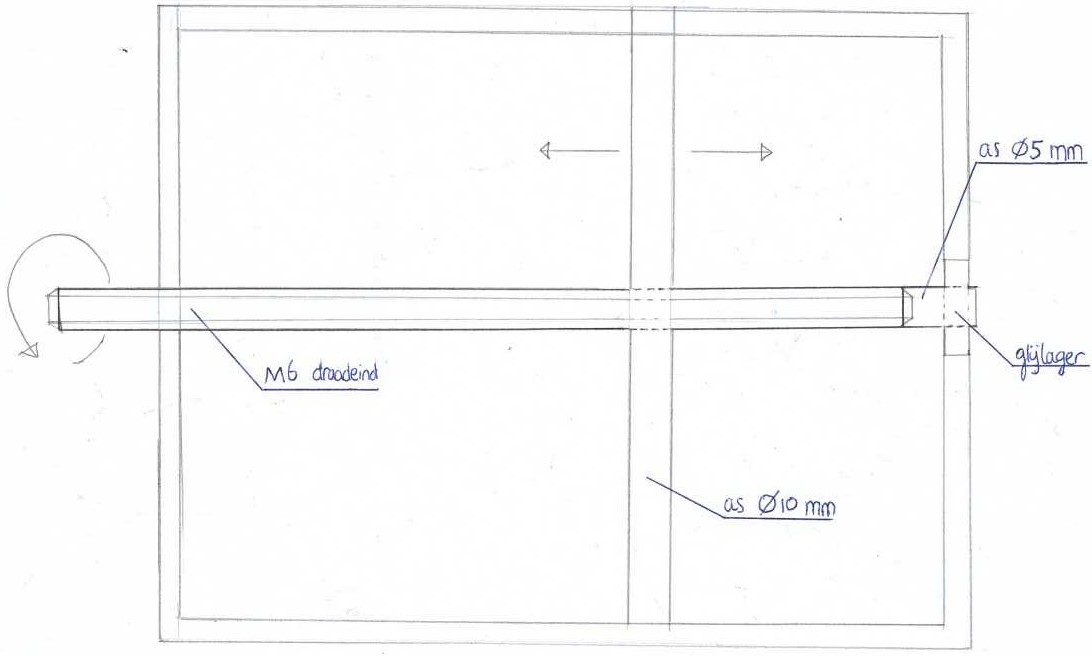
\includegraphics[width = 80mm]{04_idee_ontwikkeling/Bovenaanzicht_schaarlift.jpeg}
    \caption{Bovenaanzicht van de beweging van de schaarlift}
    \label{fig:Schaar_boven}
\end{figure}



\subsection{concept 2: \textit{Uitschuiver}}
\label{se:concept_2_uitschuiver}

De uitschuiver werkt door een stappende beweging te maken met behulp van twee schaarliften. Als de uitschuiver in de buurt van een obstakel komt wordt de achterste schaarlift uitgeklapt. Dan wordt de voorste schaarlift over het obstakel heen geschoven door het uitschuifmechanisme. Vervolgens wordt de voorste schaarlift op de grond gezet. Door het pakket vervolgens boven de bovenste schaarlift te bewegen veranderd het massamiddelpunt van het mechanisme. Als de achterste schaarlift nu opgeklapt wordt blijft het mechanisme stabiel. Ten slotte wordt de achterste schaarlift ingetrokken door het uitschuifmechanisme en kan het pakkethondje zijn weg vervolgen. Zie \cref{fig:isom_uitschuiver} voor een isometrische tekening van dit eindconcept.
\vspace{\baselineskip}

De uitschuiver wordt aangedreven door zes stepper motoren. Onder de voorste schaarlift zitten twee stepper motoren, waardoor het ontwerp kan sturen door middel van een aandrijvingsdifferentiaal. De derde stepper motor drijft de achterste schaarlift aan, waardoor de uitschuiver ook kan rijden als de voorste schaarlift niet op de grond staat. De vierde en vijfde stepper motoren drijven de schaarliften aan door een draadeind aan te draaien. De laatste stepper motor zorgt er voor dat het uitschuifmechanisme werkt. Door weer aan een draadeind te draaien kan de uitschuiver de afstand tussen de schaarliften veranderen. Om een duidelijker beeld te krijgen van de vorm van de schaarlift kan er worden gekeken naar \cref{schaarlift_hilbert}.

Bovenop de schaarlift zit het systeem dat het pakket kan verplaatsen. Door aan het touwtje met de magneet te trekken beweegt het pakket over de L-profielen. Hierdoor kan de positie van het zwaartepunt tijdens de rit aangepast kan worden. Zie \cref{fig:detail_uitschuiver} voor een tekening van het mechanisme om dit aan te passen. 


\begin{figure}[H]
    \centering
    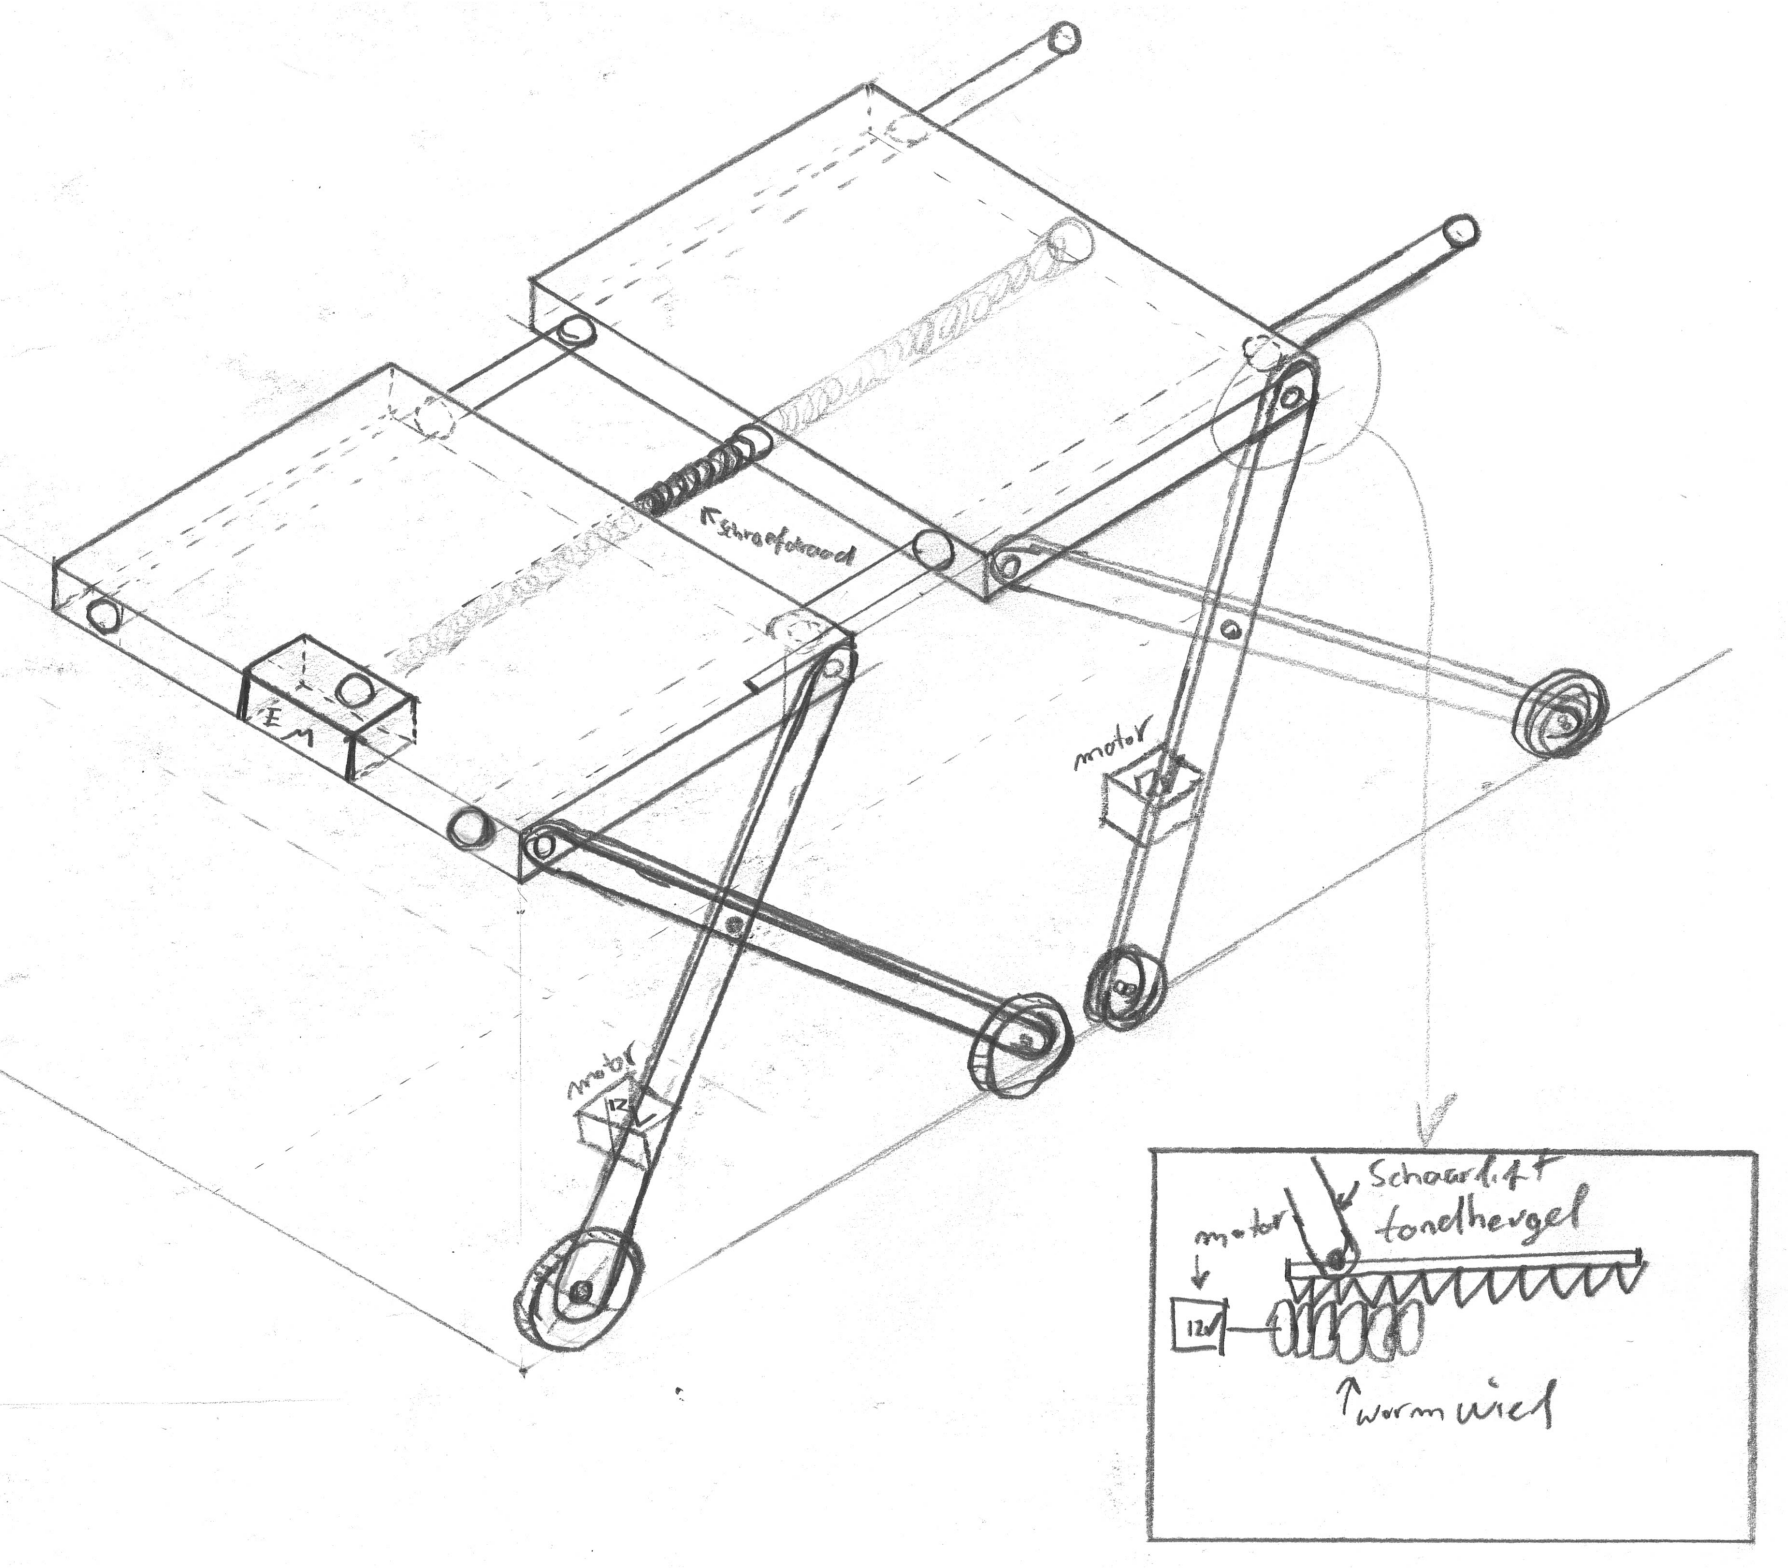
\includegraphics[width=80mm]{04_idee_ontwikkeling/isom_uitschuiver.png}
    \caption{De isometrische tekening van het concept uitschuiver}
    \label{fig:isom_uitschuiver}
\end{figure}

\begin{figure}[H]
    \centering
    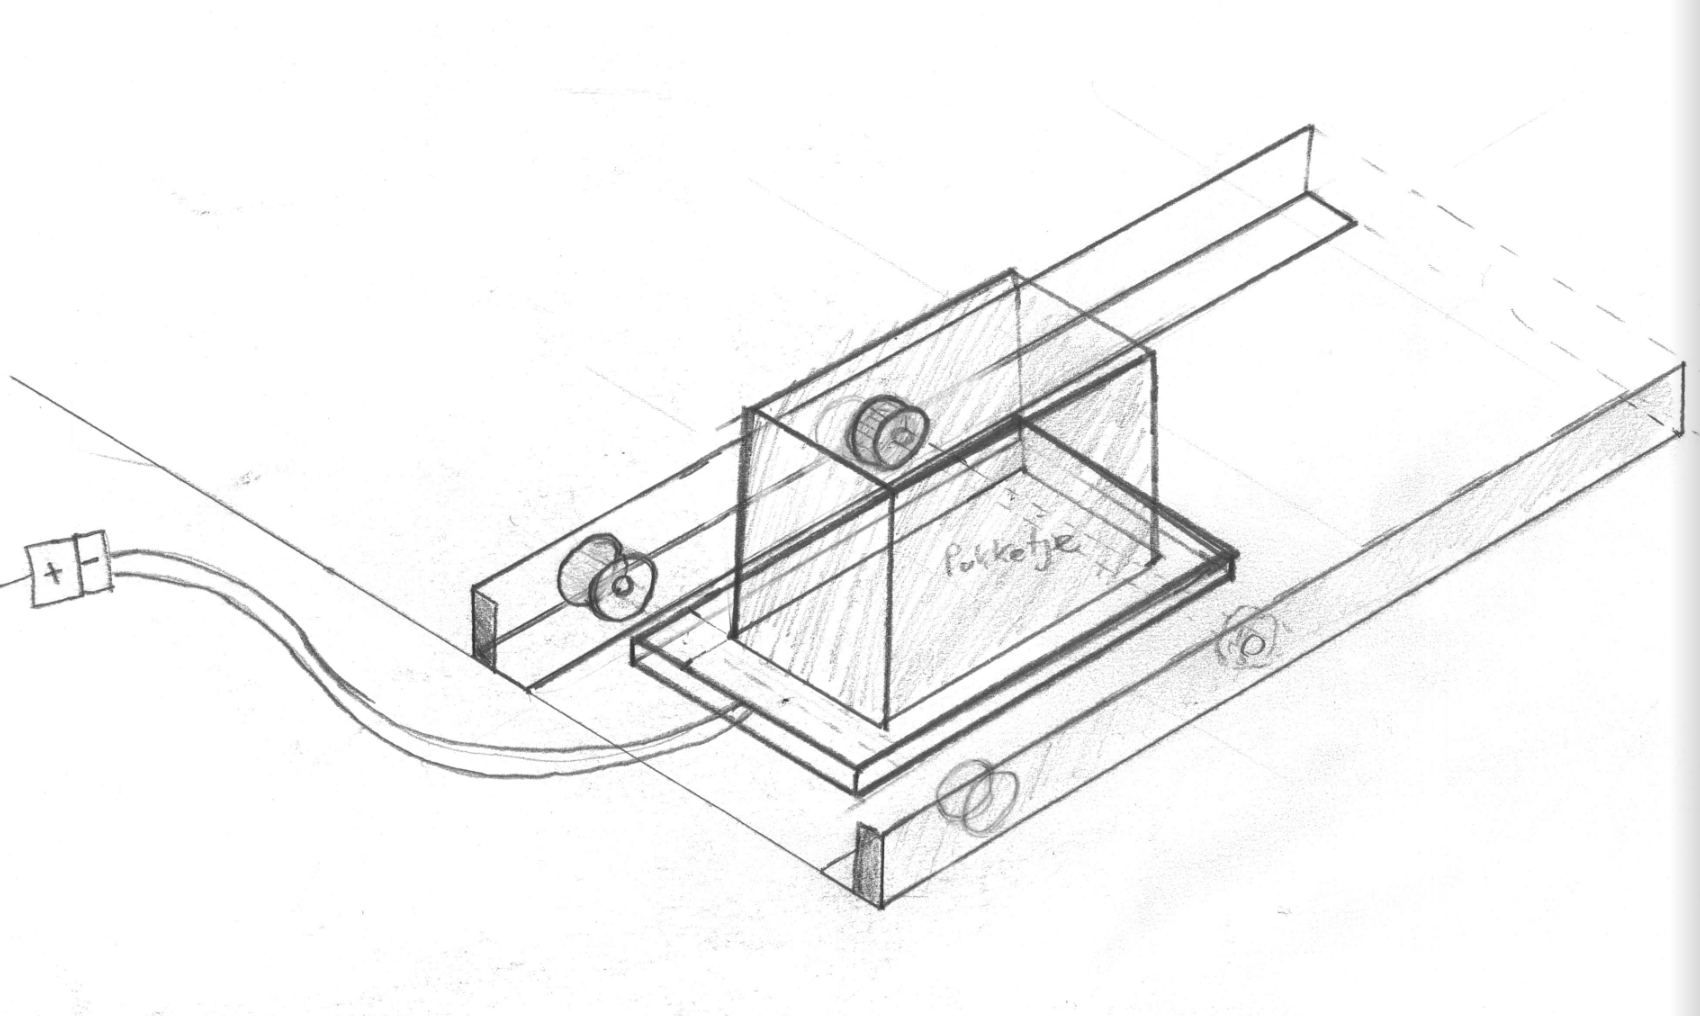
\includegraphics[width=80mm]{04_idee_ontwikkeling/detail_uitschuiver.png}
    \caption{Tekening van het mechanisme om het pakket te verplaatsen bovenop de uitschuiver.}
    \label{fig:detail_uitschuiver}
\end{figure}


\subsection{Concept 3: \textit{Inklapper}}
\label{se:inklapper}
\vspace{\baselineskip}
De Inklapper (\cref{fig:inklapper}), zoals de naam luid, bestaat uit een Plateau met 3 inklapbare wielen. Elk wiel is door middel van een schaar lift nauwkeurig op hoogte af te stellen. Het plateau heeft hierdoor de mogelijkheid in zijn geheel op/neer te bewegen, zo is het bijvoorbeeld mogelijk exact met de aanname/afgeef hoogte van het pakketje te matchen. Ook kan door de verschillende schaar liften het plateau in een hoek bewegen, ook bij een helling blijft het pakket recht. (zie \cref{fig:rechtplateau_op_helling}.)

\begin{figure}[H]
    \centering
    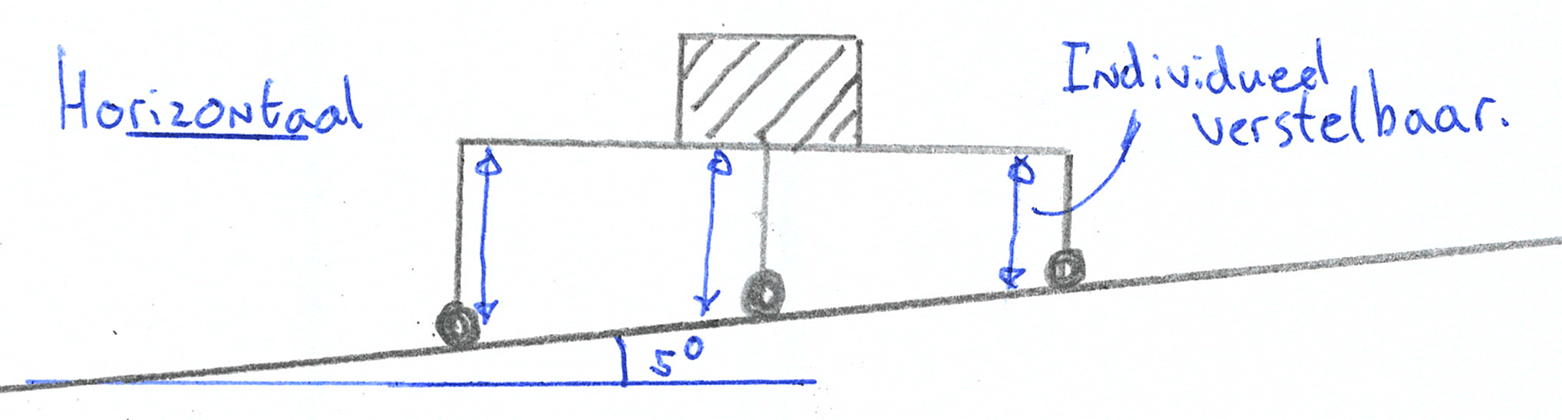
\includegraphics[width=120mm]{04_idee_ontwikkeling/Recht_onder_hoek_driepoten.png}
    \caption{Het plateau blijft recht op een schuine helling}
    \label{fig:rechtplateau_op_helling}
\end{figure}

De inklapper kan door, één van de drie wielen in te klappen zich over het obstakel bewegen. De inklapper kan zijn balans behouden door het zwaartepunt op het bewegende Plateau te verplaatsen tussen de twee overgebleven steunpunten. Het overwinnen van het obstakel gebeurd in de volgende stappen: 1 verplaatsing zwaartepunt tussen de twee steunpunten, 2 inklappen poot, 3 zich over het obstakel heen rijden, 4 uitklappen poot. Hierna herhalen deze stappen zich tot de gehele auto over het obstakel heen is. Zie \cref{fig:stappen_inklapper_met_pakket} \\


\begin{figure}[H]
    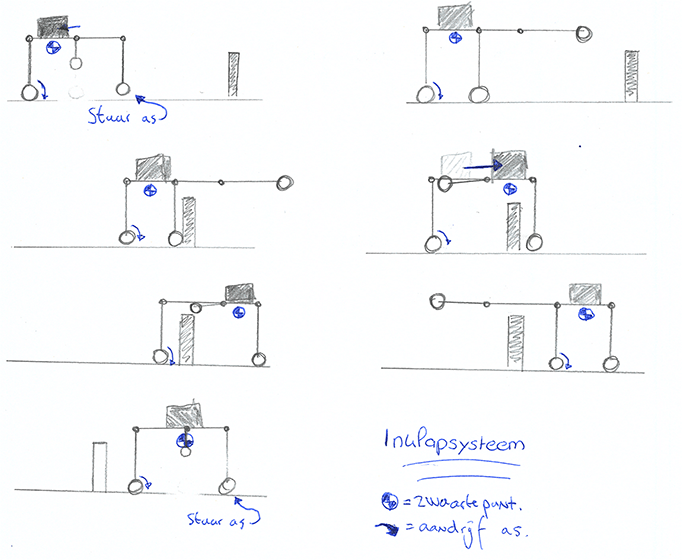
\includegraphics[width=120mm]{04_idee_ontwikkeling/Verloop_systeem_driepoten.png}
    \caption{Meerdere stappen die de in klapper onderneemt om een obstakel te overwinnen,  zwaartepunt en as die het voertuig aandrijft zijn ook aangegeven}
    \label{fig:stappen_inklapper_met_pakket}
\end{figure}

De inklapper word aangedreven door de middelste en achterste as. Het is hierdoor mogelijk altijd voor te bewegen als twee van de drie poten zich op de grond bevinden. Zie figuur \cref{fig:stappen_inklapper_met_pakket} hoe er altijd een aandrijving is om over het obstakel heen te rijden. Ook word er altijd geremd op de motor, uitgaande er nooit de noodzaak is voor een grote remkracht.  Het stuurmechanisme is gebaseerd op het Ackermann-principe (\cite{Stuurmechanisme}). De voorste poot kan met behulp van een servo en een stuur mechanisme worden bestuurd. Tijdens het rijden zal de middelste poot ingeklapt zijn, hierdoor werkt het stuurmechanisme vergelijkbaar met een auto. Dit mechanisme is in \cref{fig:vierpoter_stuursysteem} uitgewerkt. \\ 

\begin{figure}[H]
    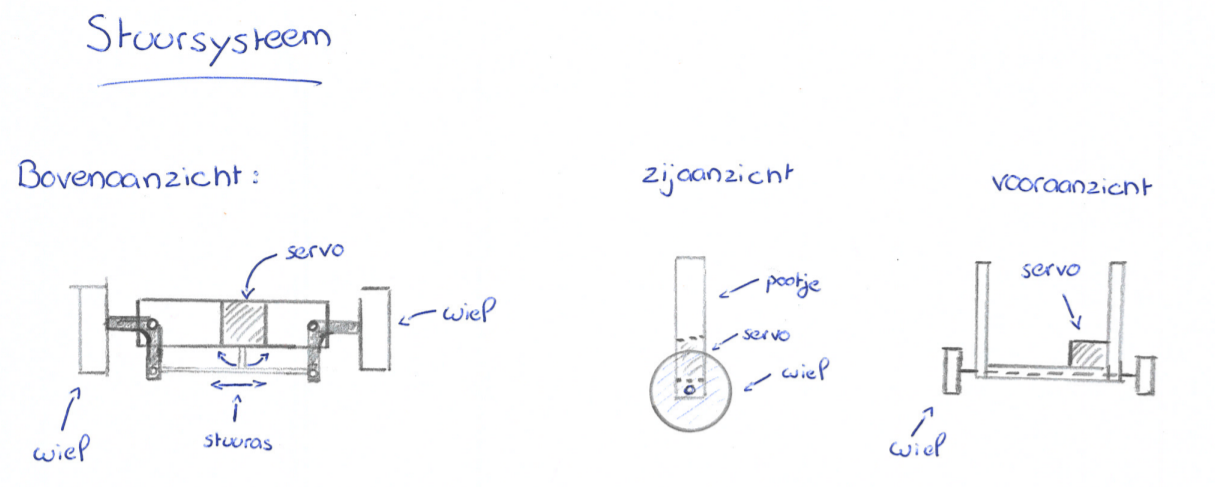
\includegraphics[width = 100mm]{04_conceptKeuze/Foto_stuursysteem.PNG}
    \caption{Concept 3, Het stuursysteem van de inklapper}
    \label{fig:vierpoter_stuursysteem}
\end{figure}

Zoals eerder vernoemd heeft het Plateau de mogelijkheid zich te verplaatsen over het dek. Aangezien het pakketje een grote massa bedraagt, heeft een verplaatsing van het plateau met pakketje direct gevolgen voor de verplaatsing van het zwaartepunt. Het plateau zit zo bevestigd op het dek dat het met weinig weerstand kan rollen, de wielen worden aan beide uit eindes geblokkeerd, zo kan het pakketje wel er af/op worden geschoven maar blijft het plateau altijd op het dek. De verplaatsing is zonder een onnodig ingewikkeld systeem maar word behulp van het touwtje met magneet verplaatst. Dit werkt nagenoeg het zelfde als \cref{se:concept_2_uitschuiver} te zien in \cref{fig:detail_uitschuiver}\\

\begin{figure}[H]
    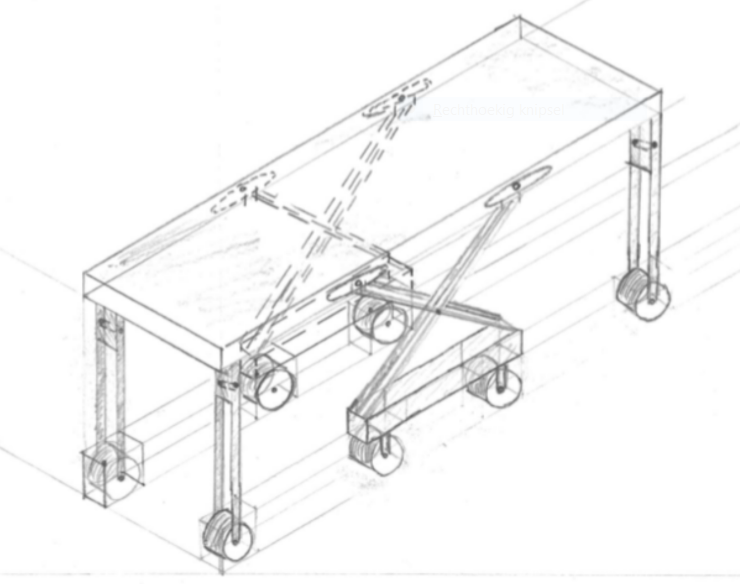
\includegraphics[width = 100mm]{Foto_inklapper.PNG}
    \caption{De inklapper}
    \label{fig:inklapper}
\end{figure}

\subsection{Concept 4: \textit{vierpoter}}
\label{se:vierpoter}
\vspace{\baselineskip}
De vierpoter heeft inklapbare pootjes waarmee hij het talud neemt. De vierpoter rijdt naar voren door de wielen, aan de onderkant, van de vier paren pootjes.\\
De voorste twee en de achterste twee worden aangedreven door vier afzonderlijke steppermotoren. \\
De onafhankelijke aandrijving zorgt ervoor dat hij kan sturen door de wielen aan een kant, de een kant op te laten draaien dan de wielen aan de andere kant. Dit zorgt ervoor dat de vierpoter een kleine bocht met een relatief hoge snelheid kan maken.  Hoe de aandrijving werkt en waar hij is bevestigd is te zien in \cref{fig:vierpoter_aandrijving}.\\

\begin{figure}[H]
    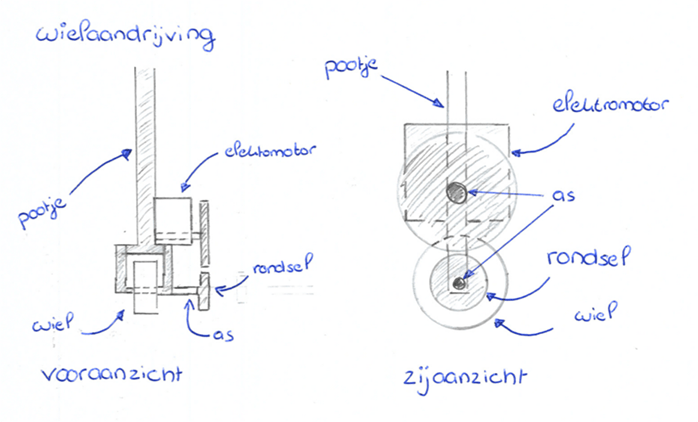
\includegraphics[width = 100mm]{04_idee_ontwikkeling/Foto_aandrijving_vierpoter.PNG}
    \caption{Concept 4, de aandrijving van de vierpoter}
    \label{fig:vierpoter_aandrijving}
\end{figure}

\vspace{\baselineskip}
Eenmaal bij het talud maakt de vierpoter gebruik van zijn inklapbare pootjes. Zijn voorste paar klappen vooruit. De vierpoter rijdt vervolgens naar voren totdat hij met zijn tweede paar tegen het talud rijdt. Nu klappen de voorste wielen weer terug en klapt het tweede paar in. Hij rijdt weer naar voren en verricht deze handeling opnieuw totdat de inklapper over het talud is. Deze handeling is te zien in \cref{fig:vierpoter_loopmechanisme}.\\

\begin{figure}[h]
    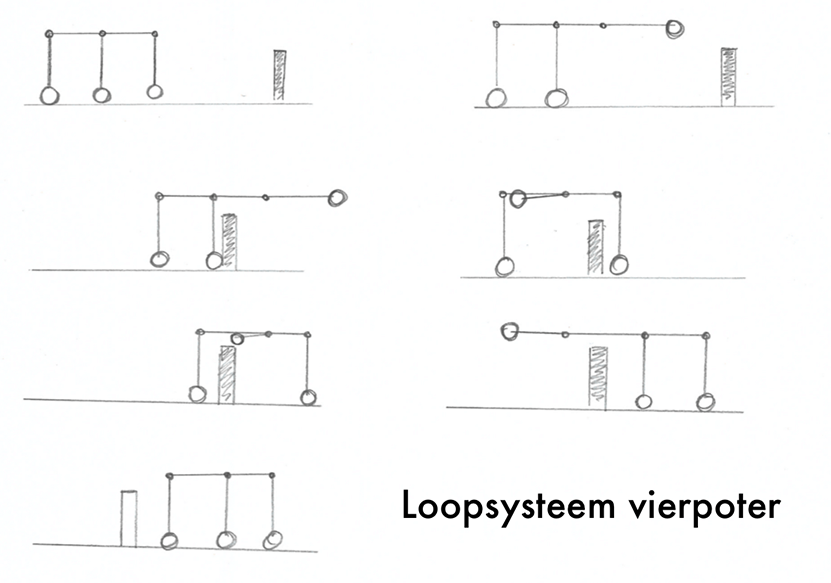
\includegraphics[width = 100mm]{04_idee_ontwikkeling/Foto_loopsysteem.PNG}
    \caption{Loop mechanisme vierpoter}
    \label{fig:vierpoter_loopmechanisme}
\end{figure}

Het inklappen van de pootjes gebeurt met behulp van een elektromotor en een tandwielen. Dit is te zien in \cref{fig:vierpoter_inklapsysteem}.\\

\begin{figure}[H]
    \centering
    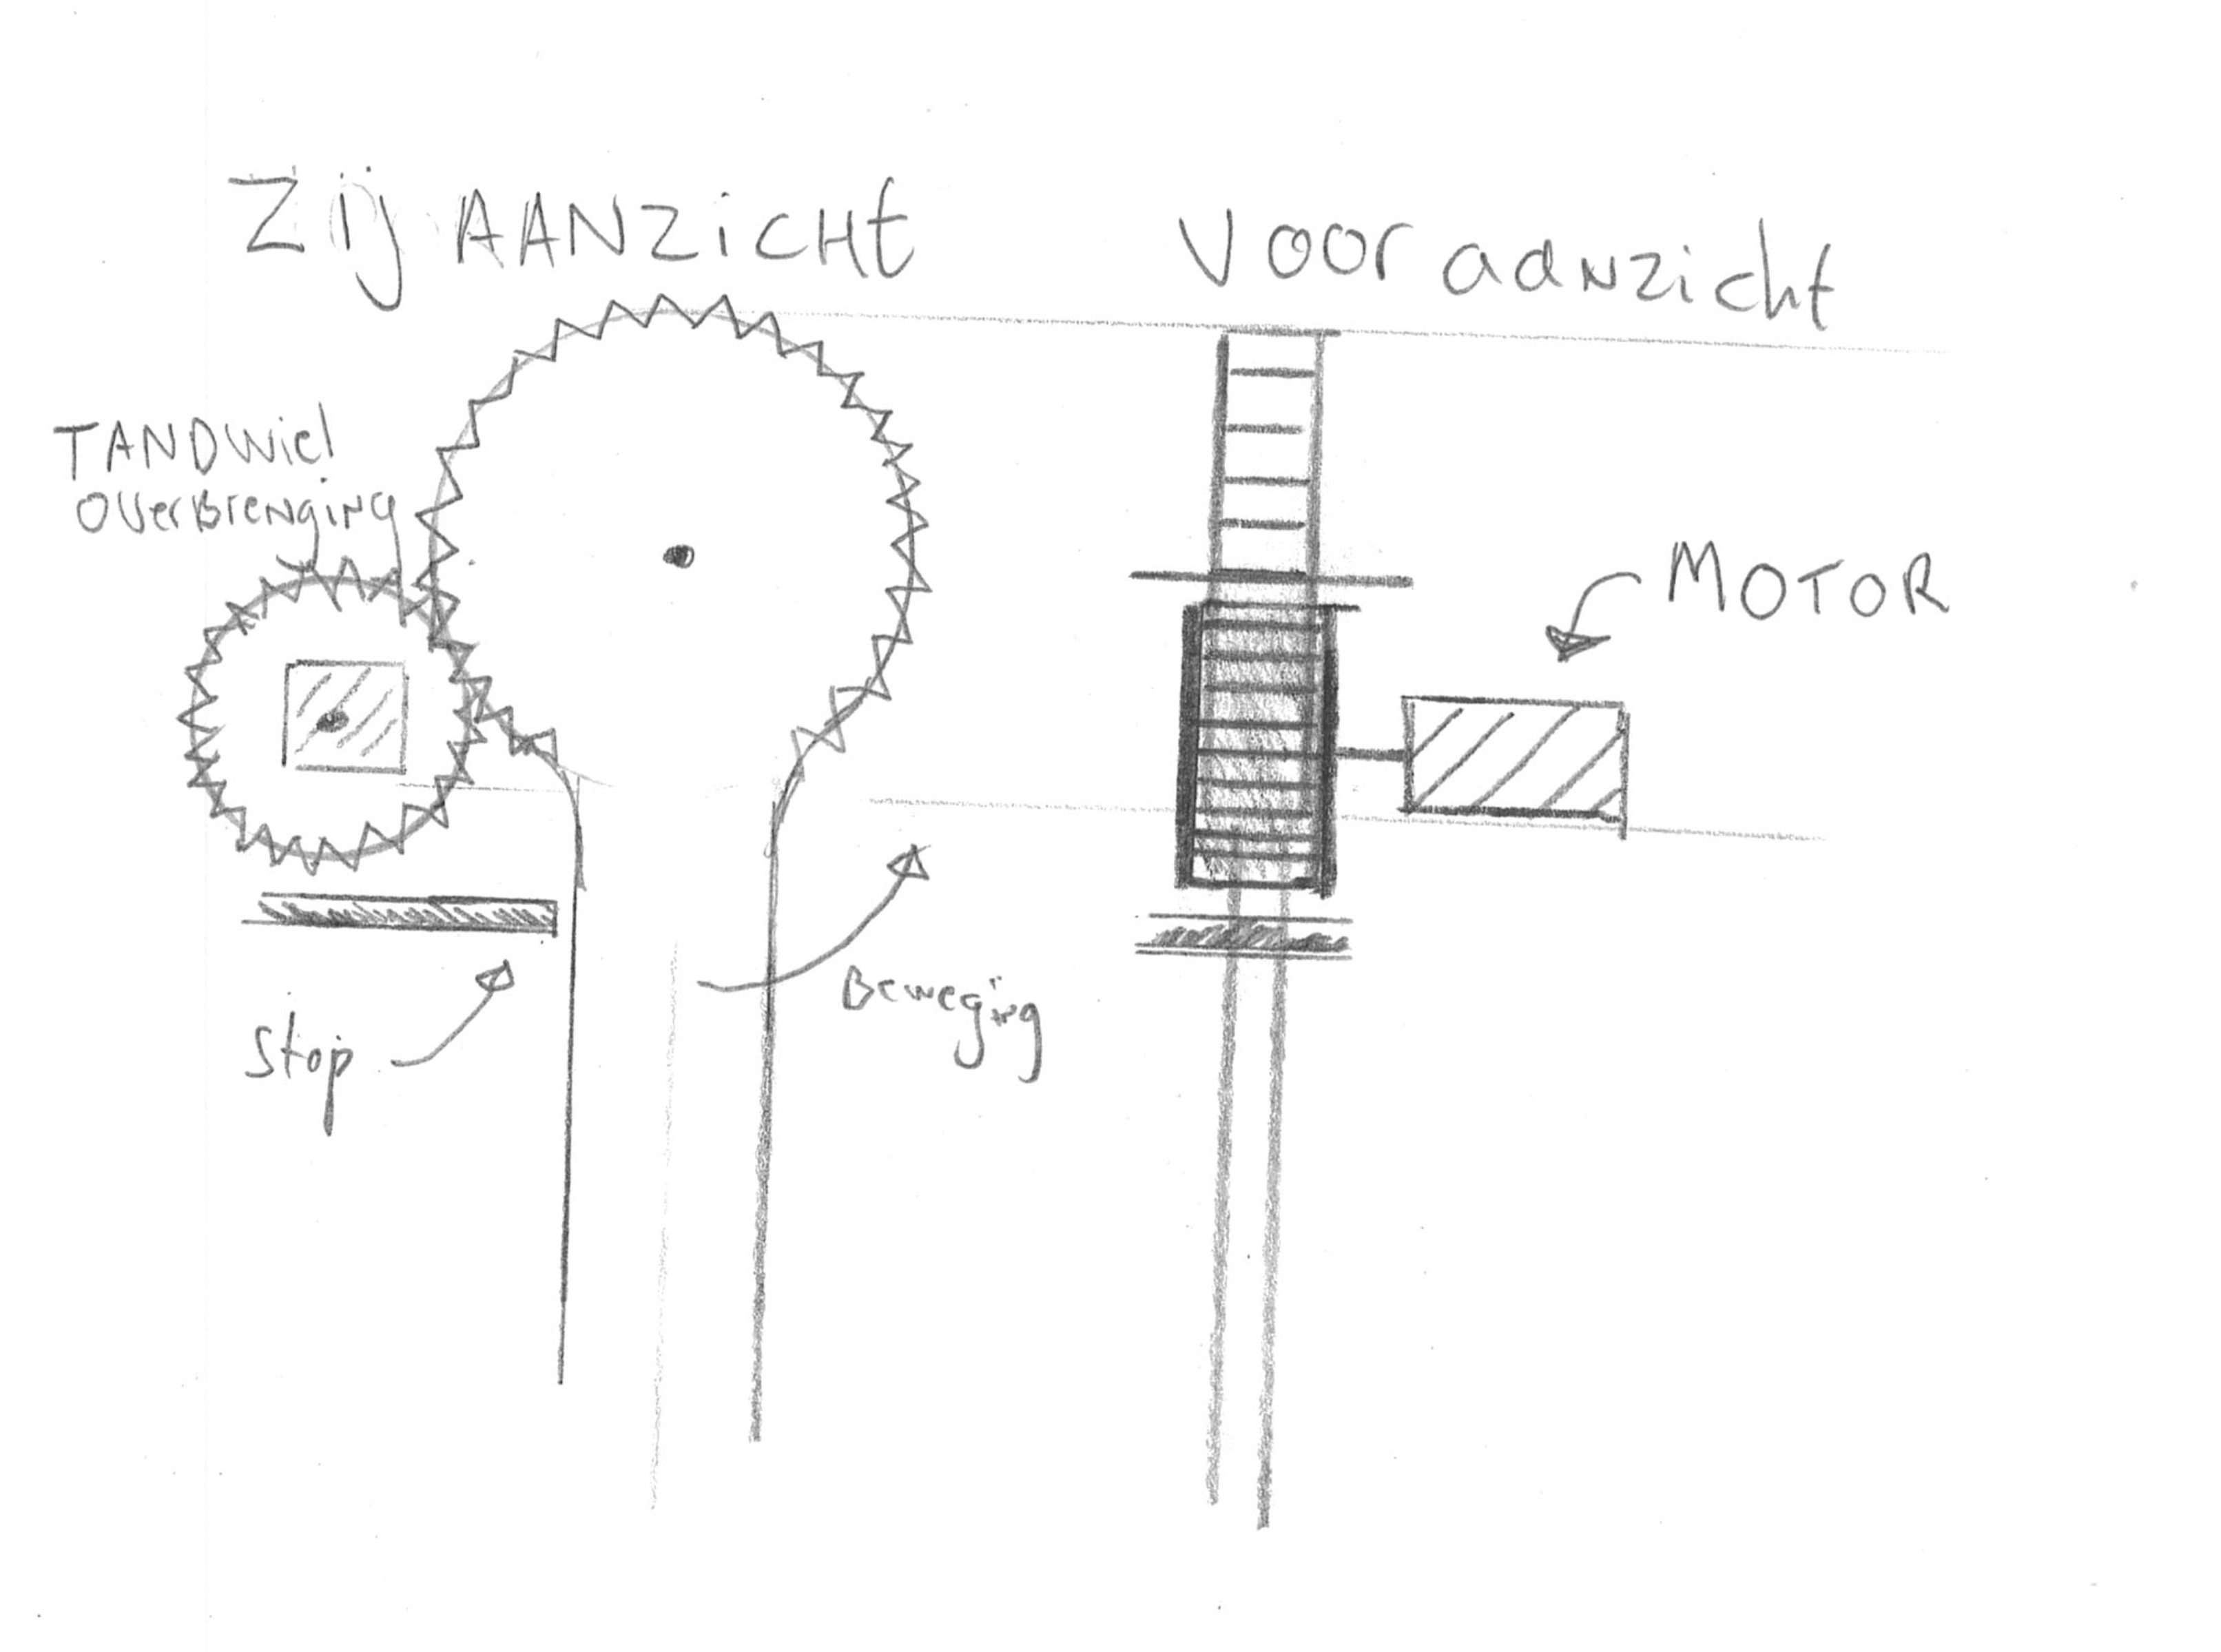
\includegraphics[width = 80mm]{04_idee_ontwikkeling/Opklapsysteem_met_tandwiel.png}
    \caption{Concept 4, inklap systeem}
    \label{fig:vierpoter_inklapsysteem}
\end{figure}

Het remmen van de vierpoter doet hij op de motor. Omdat de snelheid van de inklapper zo minimaal is en omdat er gebruik wordt gemaakt van een steppermotor is het niet nodig om remblokjes of -schijfjes toe te voegen.\\
Het ontvangen van het pakket gebeurt door middel van een rol systeem dat te zien is in \cref{fig:vierpoter_totaal}. De vierpoter is zo ontworpen dat het dezelfde hoogte heeft als het plateau waarvan hij het pakketje moet ontvangen en moet afleveren. Voor meer informatie over de vierpoter zie \cref{fig:vierpoter_totaal}. \\

 
\begin{figure}[H]
    \centering
    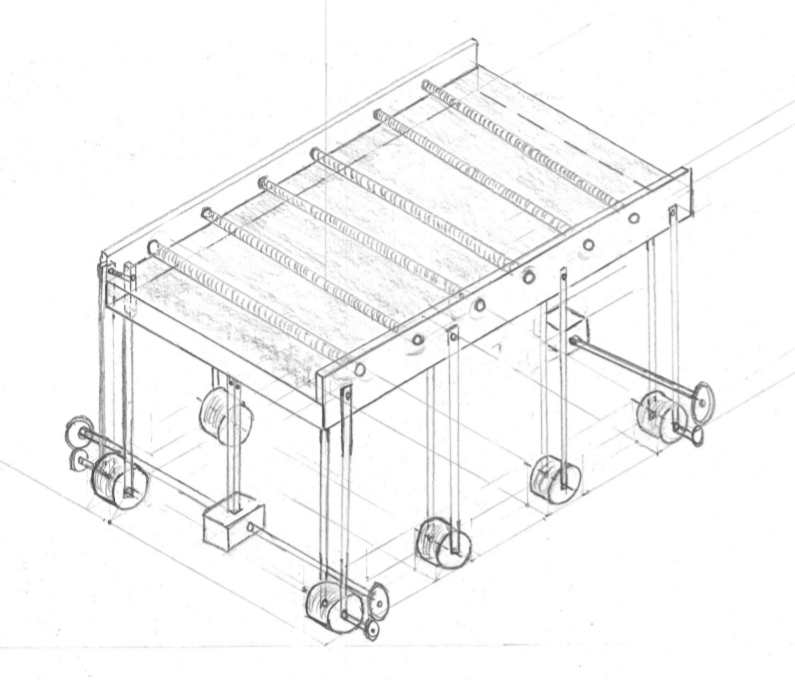
\includegraphics[width = 100mm]{04_idee_ontwikkeling/Foto_vierpoter.PNG}
    \caption{Concept 4, de vierpoter}
    \label{fig:vierpoter_totaal}
\end{figure}


\chapter{Concept Keuze}
\label{cha:Concept_keuze}

\textit{ In dit hoofdstuk worden alle concepten uit \cref{cha:ideeOntwikkeling} geanalyseerd en wordt het meest kansrijke eind concept aangewezen. Dit gebeurt op basis van het programma van eisen gegeven in \cref{se:PVE}. In \cref{se:Gewogen_criteria_methode} wordt de gewogen criteria methode toegelicht en toegepast. Dit is onderverdeeld in een stuk over de weging van de criteria (\cref{se:weging_criteria}) en een stuk toelichting over de gegeven scores (\cref{se:gegeven_scores}). Tot slot kan in \cref{se:keuze_van_concept} gevonden worden welk concept is gekozen en waarom.}

\section{Gewogen criteria methode}
\label{se:Gewogen_criteria_methode}
Uit het onderzoek van de gewogen criteria methode heeft de inklapper de hoogste score gekregen. Het maken van een concept keuze is gebeurt door middel van de gewogen criteria methode, \cite{hanus_hagger_proffitt_barnes}.

Deze methode begint met het afwegen van de gekozen prestatie criteria. Hoe belangrijk zijn de criteria ten opzichte van elkaar. Daarna krijgen de concepten scores die worden vermenigvuldigd met de weging die criteria hebben gekregen. Wat hier dan uitkomt is een ranking van verwachte prestaties van de verschillende concepten.\\


\subsection{Weging criteria}
\label{se:weging_criteria}
Voor het uitvoeren van de gewogen criteria methode is het van belang om de prestatie criteria te rangschikken op belangrijkheid. Deze rangschikking is te vinden in \cref{ch:gewogen_criteria_methode}. \\
Tijdens de afweging welke criteria belangrijker worden gevonden dan anderen, zijn er ook verschillende dilemma's naar boven gekomen. Dit zijn een paar criteria die het bespreken waard zijn:  \\

\vspace{\baselineskip}
\textbf{Wendbaarheid.} Hierin is te zien dat er een lage ranking gegeven is aan wendbaarheid. Dit komt omdat de criteria die zijn opgesteld, afgewogen zijn op de reglementen die waren gegeven aan de opdracht (\cite{beek_2020_wedstrijdregelement}). Hierdoor zijn de criteria afgewogen op hoe ze de prestatie zouden kunnen verminderen. Wendbaarheid is minder van belang omdat het meubel hondje maar twee keer 90 graden hoeft te draaien en moet kunnen bijsturen. De tijd die het concept daarvoor nodig heeft moet snel genoeg zijn maar is niet essentieel voor de prestatie van het concept.\\
\vspace{\baselineskip}

\textbf{Voorspelbaarheid.} Uit de gewogen criteria methode is naar boven gekomen dat het belangrijk is hoe voorspelbaar het meubel hondje is en hoe moeilijk het obstakel is dat hij kan nemen. De voorspelbaarheid is hoog geëindigd omdat het van belang is om te kunnen weten wat er te wachten staat. Als het ontwerp voldoende voorspelbaar is moet het ontwerp in principe voldoende kunnen worden ontworpen.\\

\textbf{Zo makkelijk mogelijk te assembleren / construeren.} Wat ook een relatief hoge score heeft gekregen is hoe makkelijk mogelijk het concept te assembleren/construeren is. Dit heeft een hoge score gekregen omdat het van belang is om een zo eenvoudig mogelijk ontwerp te krijgen. Als het concept eenvoudig wordt, is het mogelijk om het ontwerp perfect te laten functioneren. \\
\vspace{\baselineskip}



\subsection{Gegeven scores}
\label{se:gegeven_scores}
Om een concept te kiezen is het van belang om de concepten te vergelijken op de verschillende criteria. Voor de gegeven scores en het totaal aantal punten dat eruit is gekomen zie \cref{ch:gewogen_criteria_methode}. Uit deze resultaten is dat de volgende ranking eruit is gekomen: \\

\begin{center}
 \begin{tabular}{| l | c | r | }
  \hline			
  score: & concept: & punten:\\
  1 & Inklapper & 184 \\
  2 & Vierpoter & 180 \\
  3 & Mantis Car & 174 \\
  4 & Uitschuiver & 165 \\
  \hline  
 \end{tabular}
\end{center}
\vspace{\baselineskip}

Hieronder worden enkele keuzes besproken die zijn gemaakt bij het ranken van de concepten ten opzichte van elkaar:\\
\vspace{\baselineskip}

\textbf{Voorspelbaarheid concept.} Bij de voorspelbaarheid van het concept is de volgende ranking gegeven:

\begin{center}
 \begin{tabular}{| l | c | c | c | r | }
  \hline			
  x & De inklapper & De mantis car & De uitschuiver & De vierpoter \\
  Gegeven score: &  5 & 1 & 4 & 5 \\
  \hline  
 \end{tabular}
\end{center}

Bij het geven van deze scores is gekeken naar hoe het concept het talud neemt. Hoe simpeler de beweging is die het concept moet maken om over het talud te komen, hoe hoger de score bij dit criteria.\\
Daarom heeft de mantis car een lage score, het concept berust op het feit dat dit systeem zichzelf omhoog hijst door middel van een soort klauw. Deze beweging is ingewikkelder en daarom minder voorspelbaar dan een mechanisme dat als het ware over het talud stapt.\\
\vspace{\baselineskip}

\textbf{Prijs.} Bij het geven van deze scores is gekeken naar hoeveel dure onderdelen moeten worden aangeschaft per concept. De eventuele kostenposten zijn onderzocht op \cite{Conrad} en op \cite{zwaard_delft} .

Dit waren de kostenposten die uit het onderzoek naar boven kwamen: \\

\begin{itemize}
    \item Elektromotoren
    \item Arduino
    \item Hoeveelheid materiaal
    \item Accu
\end{itemize}

Hieruit blijkt dat elektra veel bepalend is voor de uiteindelijk kosten. Daarom zijn de scores voornamelijk gebaseerd op de hoeveelheid elektra en de kosten ervan. Dit zijn de gegeven scores: \\

\begin{center}
 \begin{tabular}{| l | c | c | c | r | }
  \hline			
  x & De inklapper & De mantis car & De uitschuiver & De vierpoter \\
  Gegeven score: & 4 & 5 & 2 & 4 \\
  \hline  
 \end{tabular}
\end{center}

Zoals te zien is heeft de Mantis Car een hoge score hier. Dit heeft te maken met het feit dat de mantis car gebruik maakt van maar 3 elektromotoren. In tegen stelling tot de concepten met inklapbare pootjes of schaar liften, hoeft dit concept geen pootjes in te klappen. Doordat de Mantis Car minder elektromotoren nodig heeft, heeft dit concept de hoogste score.\\ 
\vspace{\baselineskip}


\section{Keuze van Concept}
\label{se:keuze_van_concept}
Uit het onderzoek is gebleken dat op de eerste plaats de \textbf{Inklapper} is gekomen. Dit heeft te maken met de hoge scores die hij heeft gekregen bij het talud nemen en de voorspelbaarheid.\\

Dicht achter de inklapper kwam de vierpoter. In principe is een verschil van 4 punten niet doorslag gevend in de keuze van het concept. Toch is er voor de inklapper is gekozen door de aanwezigheid van een rood vlak voor de score tabel van de vierpoter. Dit rode vlak geeft aan dat de vierpoter onvoldoende scoort op het gewicht van het concept, hierdoor kan het concept wel op papier kansrijk zijn maar in praktijk is misschien het tegenover gestelde. Deze afweging heeft ervoor gezorgd dat er is gekozen voor de Inklapper.\\

\chapter{Gekozen concept}
\label{cha:gekozenConcept}

\textit{In dit hoofdstuk worden verbeterrichtingen aangewezen in het huidige ontwerp, worden de verbeteringen toegepast en wordt dit verbeterde ontwerp  geanalyseerd. Eerst worden verbeterrichtingen aangewezen vanuit het programma van eisen (\cref{se:PVE}). Dan worden deze richtingen aangevuld door het maken van een proefmodel en het uitvoeren van een veiligheidsanalyse (\ref{se:Veiligheidsanalyse}) en een faalanalyse (\cref{se:Faalanalyse}). Het verbeterde concept wordt dan toegelicht. Ten slotte wordt het verbeterde concept geanalyseerd op gewicht en bewegingsvrijheid (\cref{se:Verbeterd_concept}).}


\section{Verbeterrichtingen}
 Nadat er een keuze is gemaakt tussen de verschillende kansrijke concepten is (\cref{cha:Concept_keuze}), werd er gekeken naar hoe dit concept nog verbetert kon worden op verscheidene manieren. De pootjes die het oorspronkelijke concept bevatte, zijn veranderd voor schaarliften. Deze schaarliften staan dwars op de basis en kunnen worden bestuurd door middel van een steppermotor. 
 
 Er is gekozen voor een steppermotor, aangezien de verticale verplaatsing van de verschillende schaarliften hiermee nauwkeurig kan worden bepaald en het pakketje zo horizontaal mogelijk kan worden gehouden. De schaarliften zelf hebben als voordeel dat de hoogte van het concept hiermee kan worden veranderd, wat met de pootjes niet mogelijk was. Hierdoor is er geen extra schaarlift bovenop het concept nodig om het pakketje te kunnen ontvangen en afleveren en is het concept op deze manier een stuk simpeler geworden. Ook is het realiseren van de verticale verplaatsing met schaarliften makkelijker en was voor het omhoog- en omlaaghalen van de pootjes een redelijk ingewikkeld systeem nodig. 
 
 Voor het stuurmechanisme maakt de driepoter gebruik van het Ackermann-principe dat ook in het concept van de inklapper wordt gebruikt, zie \cref{fig:vierpoter_stuursysteem}. Het mechanisme van de wielaandrijving wordt overgenomen van de vierpoter, dit wordt afgebeeld in \cref{fig:vierpoter_aandrijving}. 
 
 \section{Veiligheidssanalyse en faalanalyse concept}
Naast een analyse van de werking van het concept, moet er uiteraard ook naar de veiligheid en faalmechanismen worden gekeken. In \cref{se:Veiligheidsanalyse} is er een analyse gedaan rondom de veiligheid van het concept. In \cref{se:Faalanalyse} is er een analyse gedaan rondom de verschillende faalemechanismen, waarbij er is gekeken naar waarschijnlijkheid van optreden en ernst van falen.

 \subsection{Veiligheidsanalyse}
 \label{se:Veiligheidsanalyse}
 Op gebied van veiligheid is er vooral aandachtig gekeken naar uitstekende en scherpe delen. 

Ten eerste werd er gekeken naar gevaren tijdens het fabriceren. In gesloten machines die door een computer wordt bestuurd, zoals een dxf snijmachine, zijn weinig gevaren. Er is weinig tot geen interactie met het materiaal zelf door de persoon. Bij bijvoorbeeld de draai- of freesmachine moet er uiteraard worden gekeken naar de bijbehorende veiligheidsvoorschriften, zoals een veiligheidsbril en een correcte jas. Er zullen ook dingen gelast moeten worden, met de bijbehorende lashelm en bedekkende kleding zou dit tot geen enkel probleem moeten lijden, er wordt extra gelet op verbrandingsgevaar (van ogen en huid). Met andere onderdelen wordt rekening gehouden dat deze niet dusdanig klein zijn dat het gevaarlijk wordt met groot gereedschap te bewerken. Na elke snij bewerking, of bij het aantreffen van een scherpe rand, wordt deze onmiddellijk geschuurd tot het de huid niet meer kan snijden.

De meeste onderdelen kunnen veilig gemonteerd worden, er zijn voornamelijk in elkaar schuivende onderdelen of in elkaar draaiende onderdelen, hier wordt geen gevaar in gezien.

Ten derde is er grondig gekeken naar de veiligheid tijdens het gebruik. Er zijn geen uitstekende onderdelen, en scherpe randen zijn keurig geschuurd of anders omgebogen. Een punt om tijdens werking op te letten zijn de schaarliften. Bij het inklappen moeten handen/voeten van de schaarlift vandaan blijven. Als het metaal naar elkaar toe beweegt ziet de steppermotor geen verschil als er er iets tussen is en kan dit verwondingen opleveren.

 
\subsection{Faalanalyse}
\label{se:Faalanalyse}
Er zijn verschillende manieren waarop het concept kan falen, maar met niet veel moeite kan met deze scenario's rekening gehouden worden en kan het risico op falen laag zijn.

Bij het driepotige concept bevindt het pakketje zich op een beweegbaar dek, hier is de kans op falen het grootst. Het dek wordt handmatig bestuurd door te trekken aan een touwtje. Dit betekend dat ten eerste het dek kan loskomen waardoor het pakketje niet meer wordt vervoerd door het pakket hondje.

Daarnaast kan er door het fout verplaatsen van het pakket hondje het zwaartepunt zich naar de verkeerde kant bewegen, dit betekent dat het gehele pakket hondje omvalt bij het nemen van een obstakel. Bij het uitoefenen van de werking van het pakket hondje kan het risico op een foute verplaatsing sterk worden verkleind. Het is dus van groot belang dat alleen personen die het concept voldoende begrijpen deze besturen.

Een ander gevaarlijk punt op falen is het bezwijken van de schaarliften onder gewicht. Dit zou betekenen het pakketje überhaupt niet kan worden overgebracht en geen obstakel zou kunnen nemen. Hierom zou hier de grootste veiligheidsmarge op moeten worden genomen. Ook al zou bij een normale veiligheidsmarge het risico niet groot zijn zou dit het gehele project kunnen ondermijnen. Er moet dus een berekening gemaakt worden om te zien of het huidige ontwerp nog aangepast moet worden voor het eindontwerp geproduceerd kan worden.
\begin{figure}[H]
    \centering
    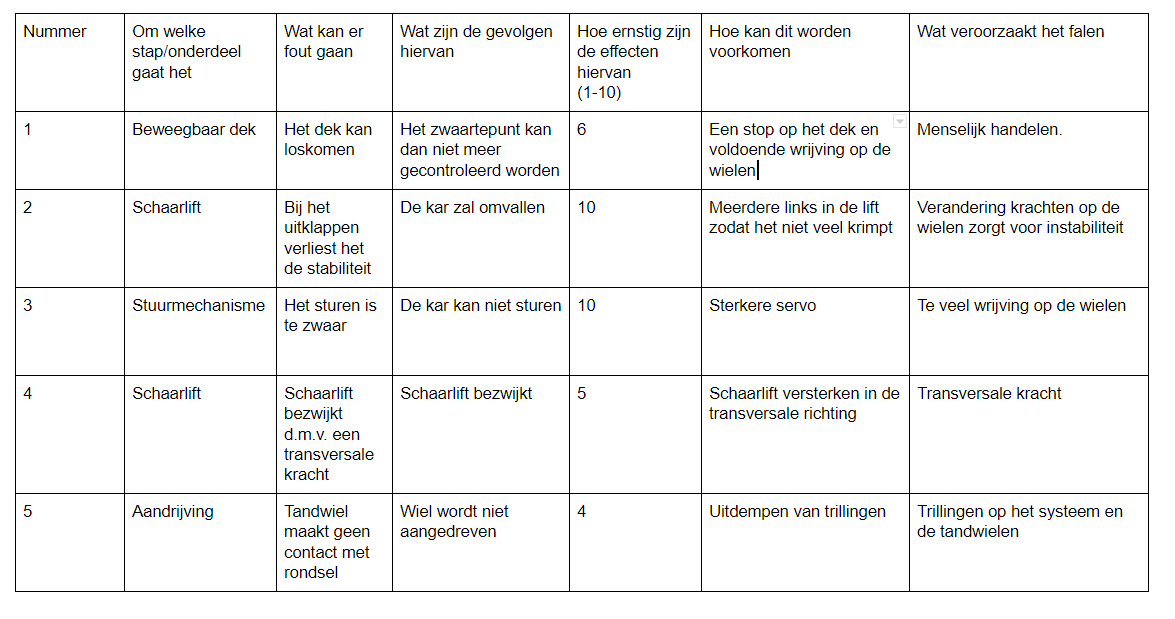
\includegraphics[width = 150mm]{04_gekozenconcept/Tabel_faal.PNG}
    \caption{Faalanalyse van de kar}
    \label{fig:tabel_faal}
\end{figure}

\section{Verbeterd concept}
\label{se:Verbeterd_concept} 
Bij dit ontwerp moet er rekening worden gehouden met de verplaatsing van het zwaartepunt, dit gebeurt door het implementeren van een schuifsysteem uit het ontwerp van de vierpoter. Dit schuifsysteem heeft een dubbele functie, namelijk: verschuiven van het zwaartepunt en bewegen van het pakketje, zie \cref{fig:driepoter_SW} voor verheldering op het mechanisme. 

Door het model in solidworks te maken is de massa van het ontwerp bekend. Volgens solidworks is dit ongeveer 8kg. Dit is minder dan het pakket, wat betekend dat het zwaartepunt van het ontwerp makkelijk aangepast kan worden door het bewegen van het pakket.

Ook kan de bewegingsvrijheid van het model ingeschat worden met behulp van het solidworks model. In het huidige ontwerp heeft elke schaarlift 4 links van 300mm lang. Hierdoor kan het ontwerp obstakels van meer dan 30cm hoog en 30cm breed nemen.

\begin{figure}[H]
    \centering
    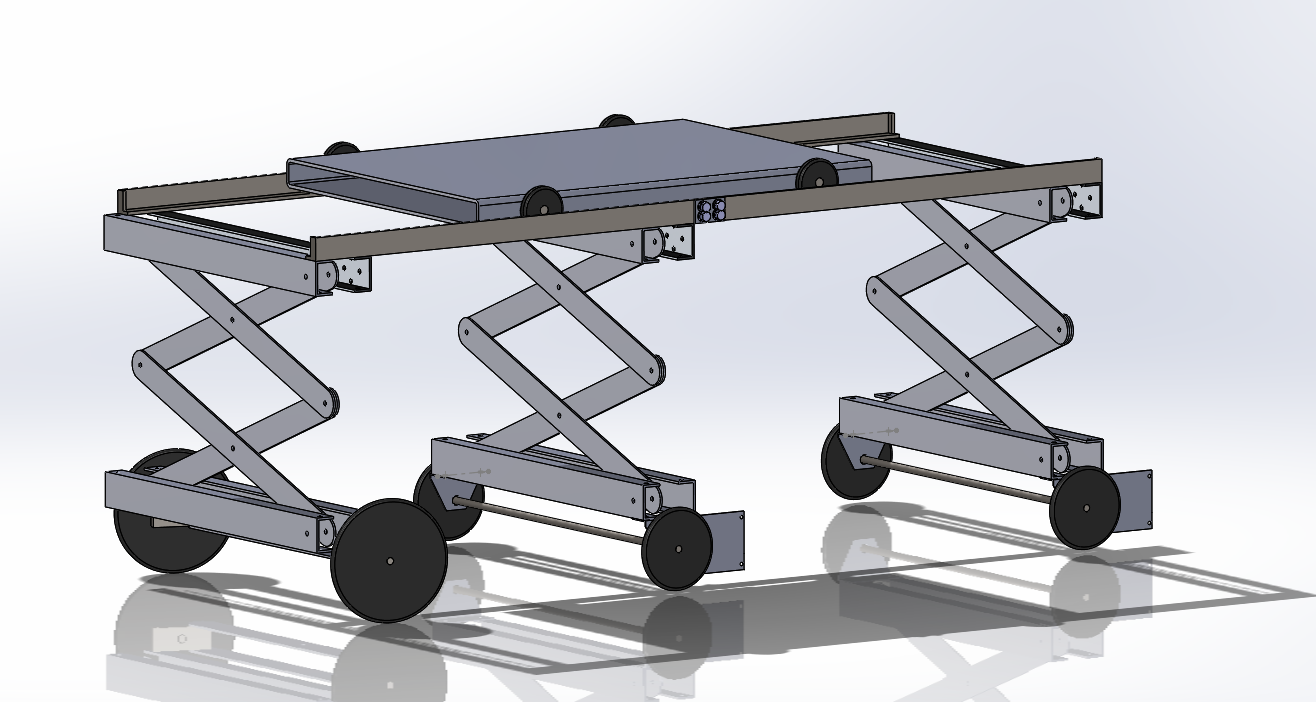
\includegraphics[width = 100mm]{04_gekozenconcept/eindconcept.png}
    \caption{3D-model Driepoter}
    \label{fig:driepoter_SW}
\end{figure}

In \cref{cha:bijlage_C} zijn de aanzichten van de driepoter afgebeeld met de bijbehorende hoofdmaten. 


\chapter{Conceptdimensionering}
%In dit hoofdstuk: kritische onderdelen, maak- en koopdelen, toleranties, verbeterde SW-model.
\label{Concept_dimensionering}
\textit{In dit hoofdstuk wordt er verder gekeken naar de specifieke concept-dimensionering. Hierbij worden de kritische onderdelen vastgesteld en vervolgens berekent op sterkte en stijfheid (\cref{se:kritische_onderdelen}). Uit deze berekeningen volgen de dimensies. \\
Als de dimensies zijn afgerond wordt er een maak- en kooplijst gemaakt. Bij het opstellen van deze lijsten wordt er rekening gehouden met de geometrie, dimensies en materiaalkeuze op basis van de berekeningen.}


\section{Kritische onderdelen.}
\label{se:kritische_onderdelen}
In dit deel van het hoofdstuk wordt gekeken naar welke onderdelen mogelijke kritische onderdelen zijn en de dimensionering ervan. Eerst worden de kritische onderdelen vastgesteld en worden er aannames gemaakt over hoe deze onderdelen worden belast \cref{se:onderdelen_met_toelichting}. In \cref{se:werking_kritische_onderdelen} worden de kritische onderdelen verder toegelicht. Er wordt kort verteld hoe ze in elkaar zitten en werken. In \cref{se:berekening_en_dimensionering} wordt er gekeken naar de dimensionering en worden de berekeningen aan de verschillende kritische onderdelen uitgewerkt.
\vspace{1mm}

\subsection{De onderdelen met toelichting.}
\label{se:onderdelen_met_toelichting}
De onderdelen die de grootste kans op falen hebben zijn:

\begin{description}
    \item \textbf{De wielassen.} De keuze van de wielassen als kritisch onderdeel is gemaakt vanwege het grote gewicht dat op de assen komt te staan. Een as moet vanwege de werking van het pakket hondje tijdens het nemen van het talud de helft van het totale gewicht kunnen hebben. \\

    \item \textbf{De schaarliften.} Dit onderdeel is essentieel voor de werking van het mechanisme. De krachten op de members van de schaarlift zijn mogelijk erg groot, daarom is het nodig om te kijken welke krachten spelen in deze members om ze goed te kunnen dimensioneren.\\

    \item \textbf{De motoren.}
    
    \item \textbf{Het stuursysteem.} Voor het verloop van het parcours is het van belang er bochten gemaakt kunnen worden, dit wordt gedaan met het Ackermann stuursysteem. Door vele bewegende onderdelen is het van belang dat dit niet bezwijkt onder druk, ook moet er berekend worden of de scherpe hoek kan worden gemaakt (met eventueel paar keer steken).\\
    
    \item \textbf{L-profiel aan de bovenkant van de kar.}

    \item \textbf{U-profiel aan de onderkant van de kar.} Aan de onderkant van de kar moeten de schaarliften worden bevestigd samen met de motoren en de wielen. Dit onderdeel moet dus goed op stijfheid worden gedimensioneerd omdat het essentieel is dat dit onderdeel niet vervormd met alle gevolgen van dien.\\ 
\end{description}

\vspace{\baselineskip}
\subsection{Werking en functie kritische onderdelen.}
\label{se:werking_kritische_onderdelen}

\textbf{De wielassen.}\\
Aan de onderkant van het pakket hondje hebben wij wielen gemaakt, deze wielen worden op hun plek gehouden door middel van assen. Deze assen worden aangedreven en moet er voor zorgen dat het pakkethondje zich voortbeweegt.\\
\vspace{\baselineskip}

\textbf{De schaarliften.}\\
Een essentieel onderdeel voor de werking van ons talud-neem-mechanisme zijn de schaarliften. Door een schaarlift op te klappen en die over het talud te rijden is het pakket hondje in staat om als het ware over het talud te stappen.\\
\vspace{\baselineskip}

\textbf{De motoren}

\textbf{Ackermann-stuursysteem.}\\
Bij het ackermann stuursysteem wordt er uitgegaan van het Ackermann principe: de wielen op de as maken altijd een hoek van 90 graden ten opzichte van een bepaald punt wat achter de as ligt. De wielen moeten met behulp van fusees zijn bevestigd met de wielas, omdat de starre as niet kan meedraaien en dit ook niet de bedoeling is. De fusees zijn verbonden met een andere as, niet de wielas, welke voor de uiteindelijke draairichting zorgt, zie \cref{fig: ackermann_FBD}. Deze as wordt aangedreven d.m.v. een servomotor en zo kan de bochtstraal/bocht richting worden bepaald. Deze servo is niet weergegeven in \cref{fig: ackermann_FBD} maar zal wel in ons concept komen. De bochtstraal hangt ook af van de achterste wielas. Deze wielen draaien niet mee en dus wordt er voor de bochtstraal uitgegaan van de hartlijn van de achterwielen. De wielen dienen minimaal zodanig te draaien dat ze loodrecht staan op het punt waar je omheen wil draaien, in de afbeelding de ‘centre of turning’.\\

\begin{figure}[H]
    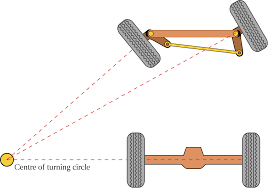
\includegraphics[width = 100mm]{04_conceptdimensionering/ackermann.png}
    \caption{Ackermann Stuursysteem, }
    \label{fig: ackermann_FBD}
\end{figure}

\vspace{1mm}
\textbf{L-profiel aan de bovenkant van de kar.}

\vspace{1mm}
\textbf{U-profiel aan de onderkant van de kar.}\\
De wielassen en de schaarliften moeten aan elkaar worden bevestigd, dit doet het u-profiel aan de onderkant van de kar. Hier worden ook de motoren bevestigd die de wielassen aandrijven.\\

\vspace{1mm}
\subsection{Berekeningen en dimensionering}
\label{se:berekening_en_dimensionering}
\vspace{\baselineskip}

\textbf{De wielassen}.\\
Er is gerekend aan de assen en de conclusie is dat een 6/8 mm as van staal voldoet. De berekening is gemaakt in een python script, zie \cref{Cha: Bijlage_F}.\\
\vspace{\baselineskip}
De berekening is als volgt opgezet:\\
Om aan de situatie te kunnen rekenen, moest eerst de situatie versimpeld worden en tot een reëel FBD worden gebracht, zie \cref{fig: as_FBD}. Hier is aangenomen dat je de as kan beschouwen als een aan twee kanten ingeklemde balk. Ook is F niet P, door een verdeling van gewicht. Deze verdeling is bekend.

\begin{figure}[H]
    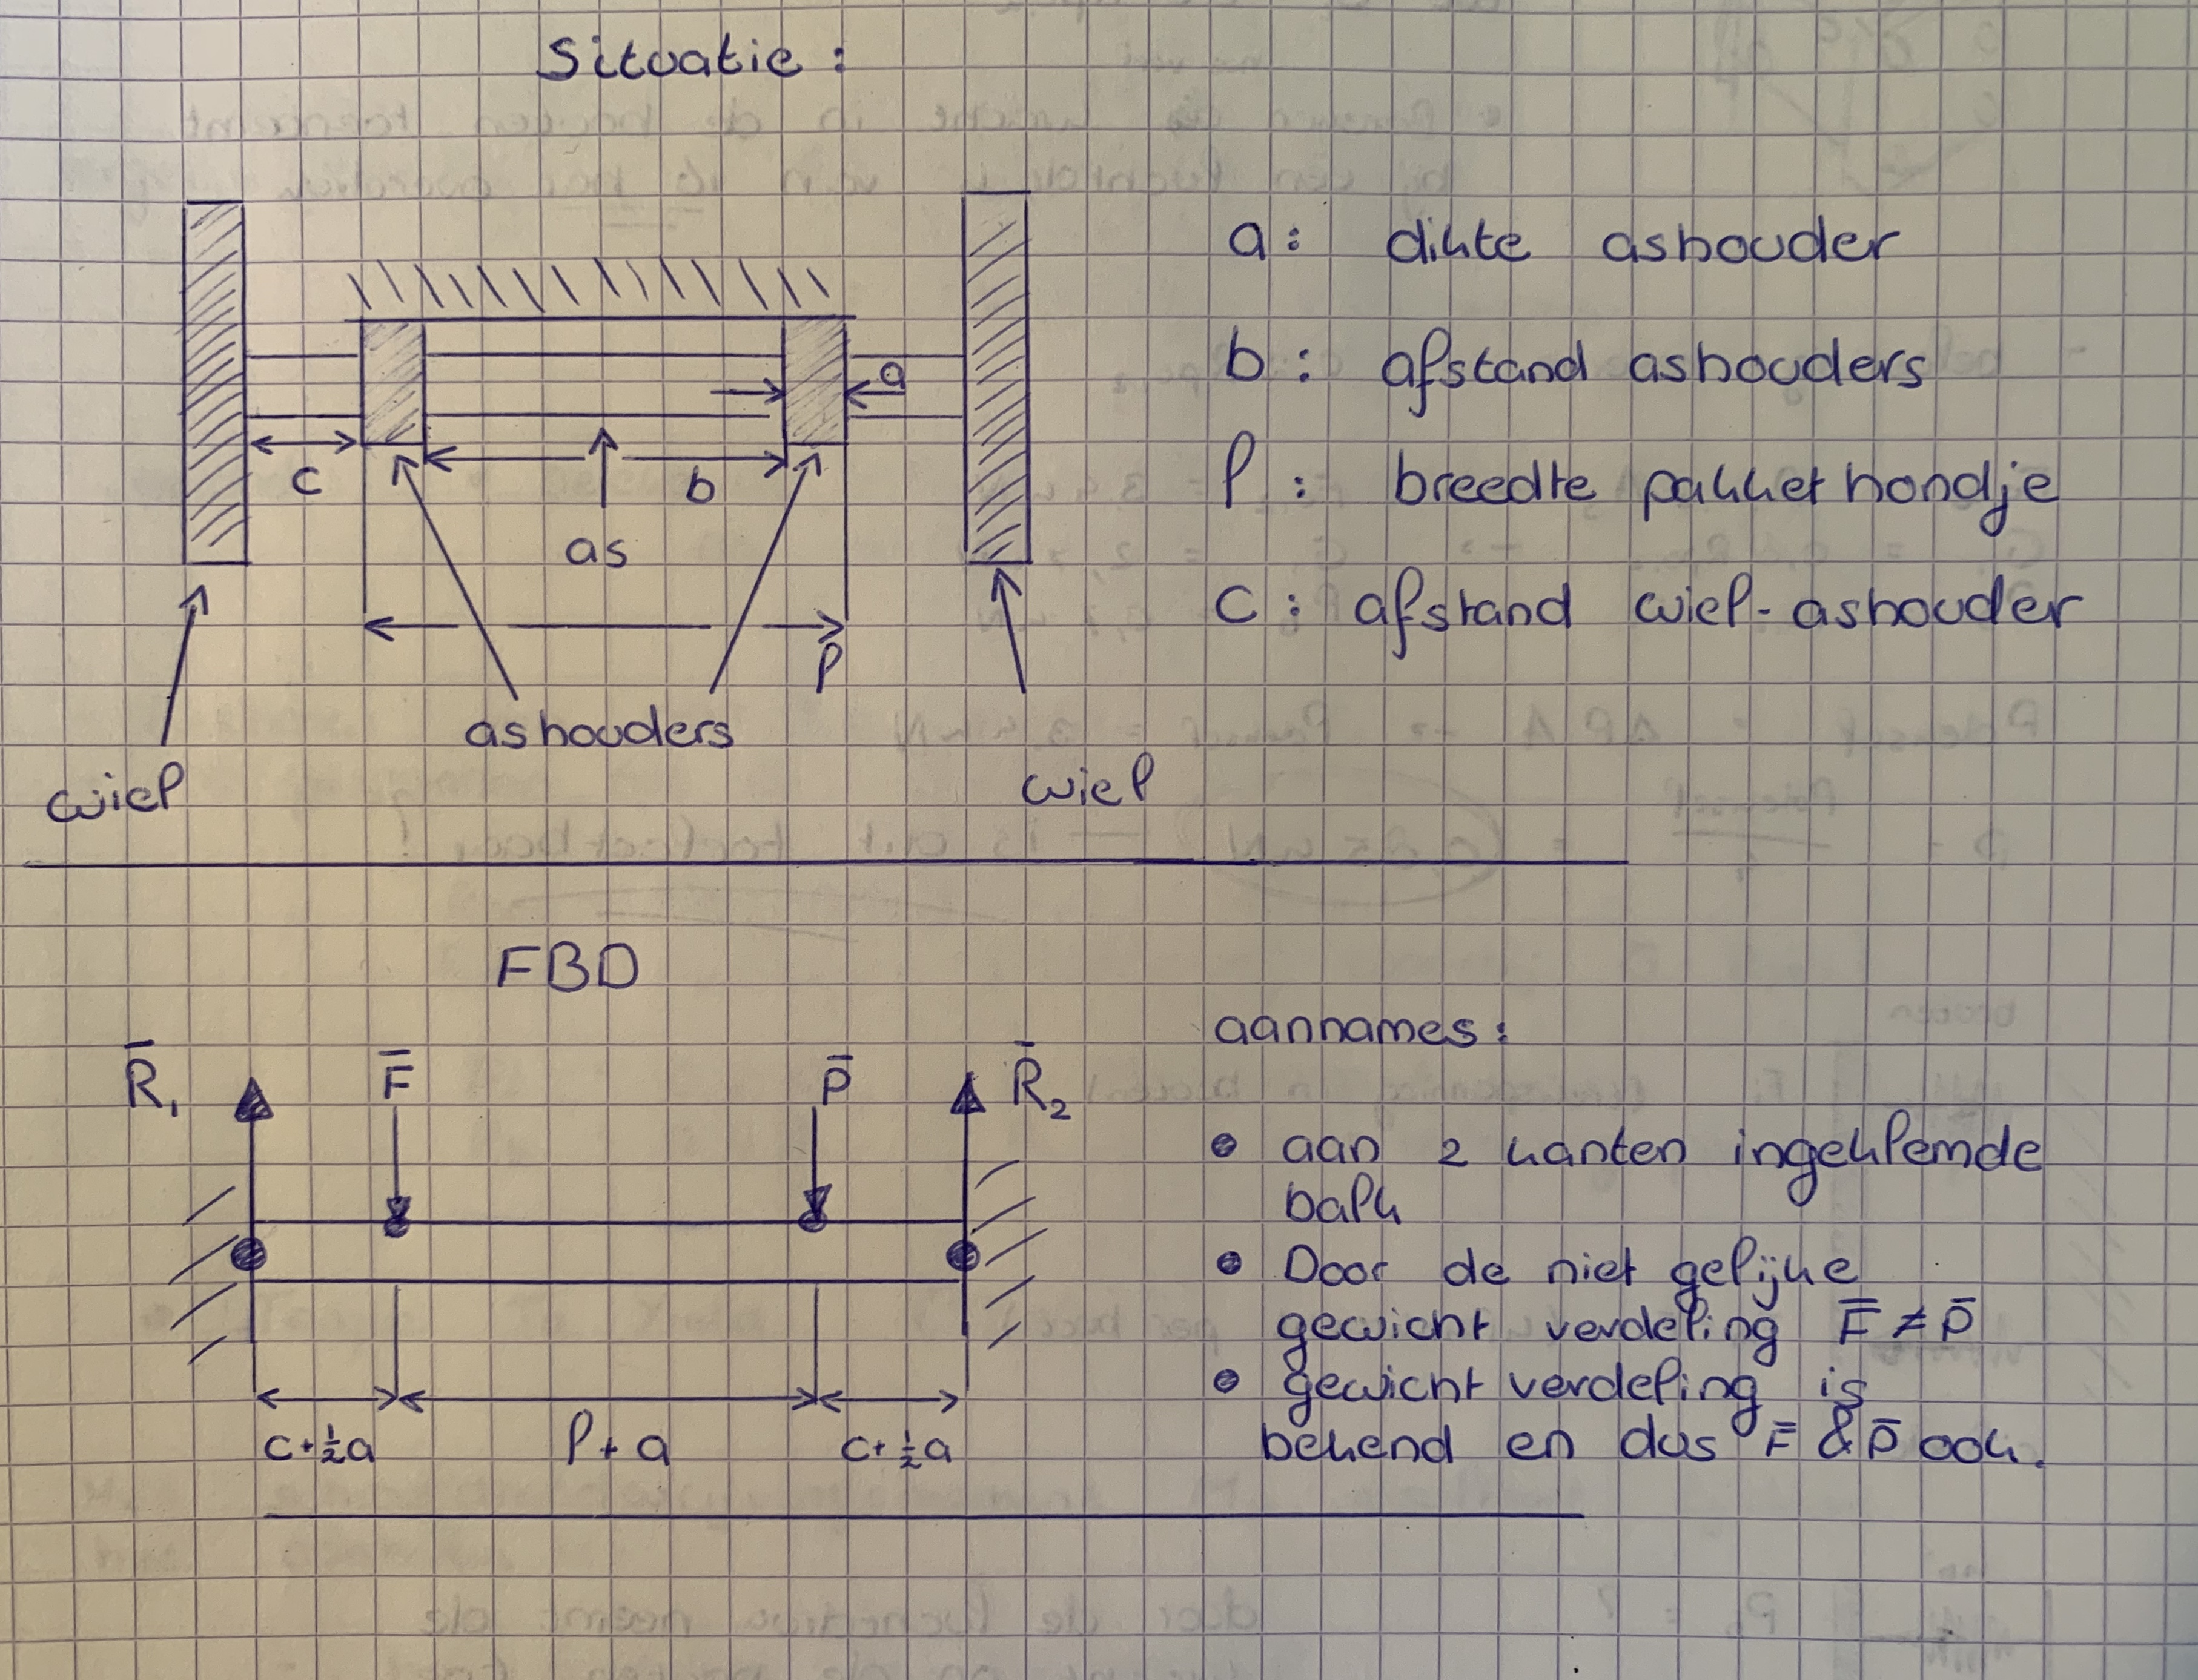
\includegraphics[width = 100mm]{04_conceptdimensionering/As_FBD.jpg}
    \caption{Bepaling van het FBD van de as.}
    \label{fig: as_FBD}
\end{figure}

Door middel van de snede methode kan je vervolgens de krachten en momenten lijn opstellen, deze berekening is te zien in \cref{Cha: Bijlage_F}. In \cref{fig: as_constanten} zijn de constanten te zien die zijn gebruikt voor het bepalen van de momenten en krachten lijn. Deze constanten hebben geleid tot de momenten en krachten lijn die te zien zijn in \cref{fig: Momentenlijn_as} en \cref{fig: Krachtenlijn_as}. \\

\begin{figure}[H]
    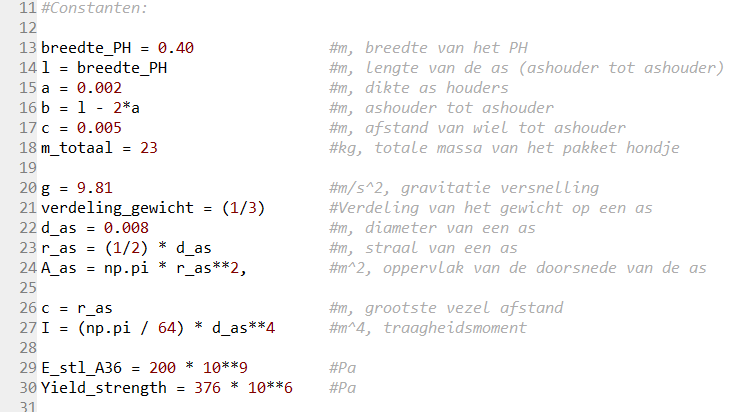
\includegraphics[width = 100mm]{04_conceptdimensionering/Constanten_as_goed.PNG}
    \caption{Constanten van de as.}
    \label{fig: as_constanten}
\end{figure}

\begin{figure}[H]
    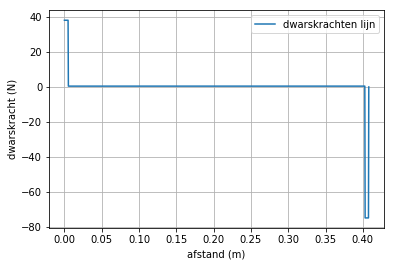
\includegraphics[width = 100mm]{04_conceptdimensionering/Krachtenlijn_as.png}
    \caption{Krachten lijn in de as.}
    \label{fig: Krachtenlijn_as}
\end{figure}

\begin{figure}[H]
    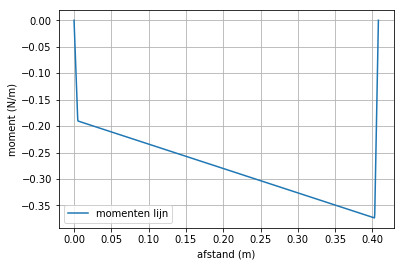
\includegraphics[width = 100mm]{04_conceptdimensionering/Momentenlijn_as.png}
    \caption{Momenten lijn in de as.}
    \label{fig: Momentenlijn_as}
\end{figure}


\textbf{De schaarliften.}\\
Ook aan de schaarliften zijn gerekend en de conclusie is dat de schaarliften een koker-profiel krijgen, met dit profiel en een gepaste lengte kan een member van de schaarlift de krachten hebben.\\
Voor de schaarliften is naar een aantal dingen gekeken:\\
\vspace{\baselineskip}
\begin{enumerate}
    \item \textbf{De vorm van belasting.} Er is een FBD van de schaarlift en van een members opgesteld om te kijken naar de vorm van de belasting op de onderdelen, zie \cref{fig: FBD_member}. Uit deze FBD kan worden geconcludeerd dat de members van de schaarlift op zuivere druk worden belast. Hierdoor moet rekening worden gehouden met knik en met de druksterkte van het materiaal.\\
    \item \textbf{De mate van belasting.} Om te bepalen wat de grootte van de belasting is moeten de krachten worden ontleden. Gebleken is na onderzoek door middel van een python script (\cref{se: bijlage_F schaarliften}) dat de members de belasting kunnen hebben. Uit het script worden bepaalde conclusies getrokken die te vinden zijn in \cref{fig: Kernel_schaarlift_1} en \cref{fig: Kernel_schaarlift_2}.\\
    \item \textbf{Het profiel van de members.} Uit het onderzoek is gebleken dat de members op een zuivere druk worden belast. Dit betekend dat er niet voor een specifiek profiel hoeft worden gekozen mits het oppervlak van een doorsnede groot genoeg is. Toch hebben wij voor een koker-profiel gekozen omdat naast de verwachtte krachten langs de members het ook waarschijnlijk is dat er krachten zullen opspelen in andere richtingen. Daarom is voor de zekerheid gekozen voor een koker profiel met de dimensionering die te vinden is in \cref{fig:schaarliften_constanten} in \cref{se: bijlage_F schaarliften}. Ook zijn hier berekeningen mee gedaan die te vinden zijn in \cref{fig: Kernel_schaarlift_2}.\\
    \item \textbf{De dimensionering van de members.} De dimensionering van de members zijn uit het python script gehaald, die zijn te vinden in \cref{fig:schaarliften_constanten} en in \cref{fig: Kernel_schaarlift_1}.
\end{enumerate}
\vspace{\baselineskip}

\begin{figure}[H]
    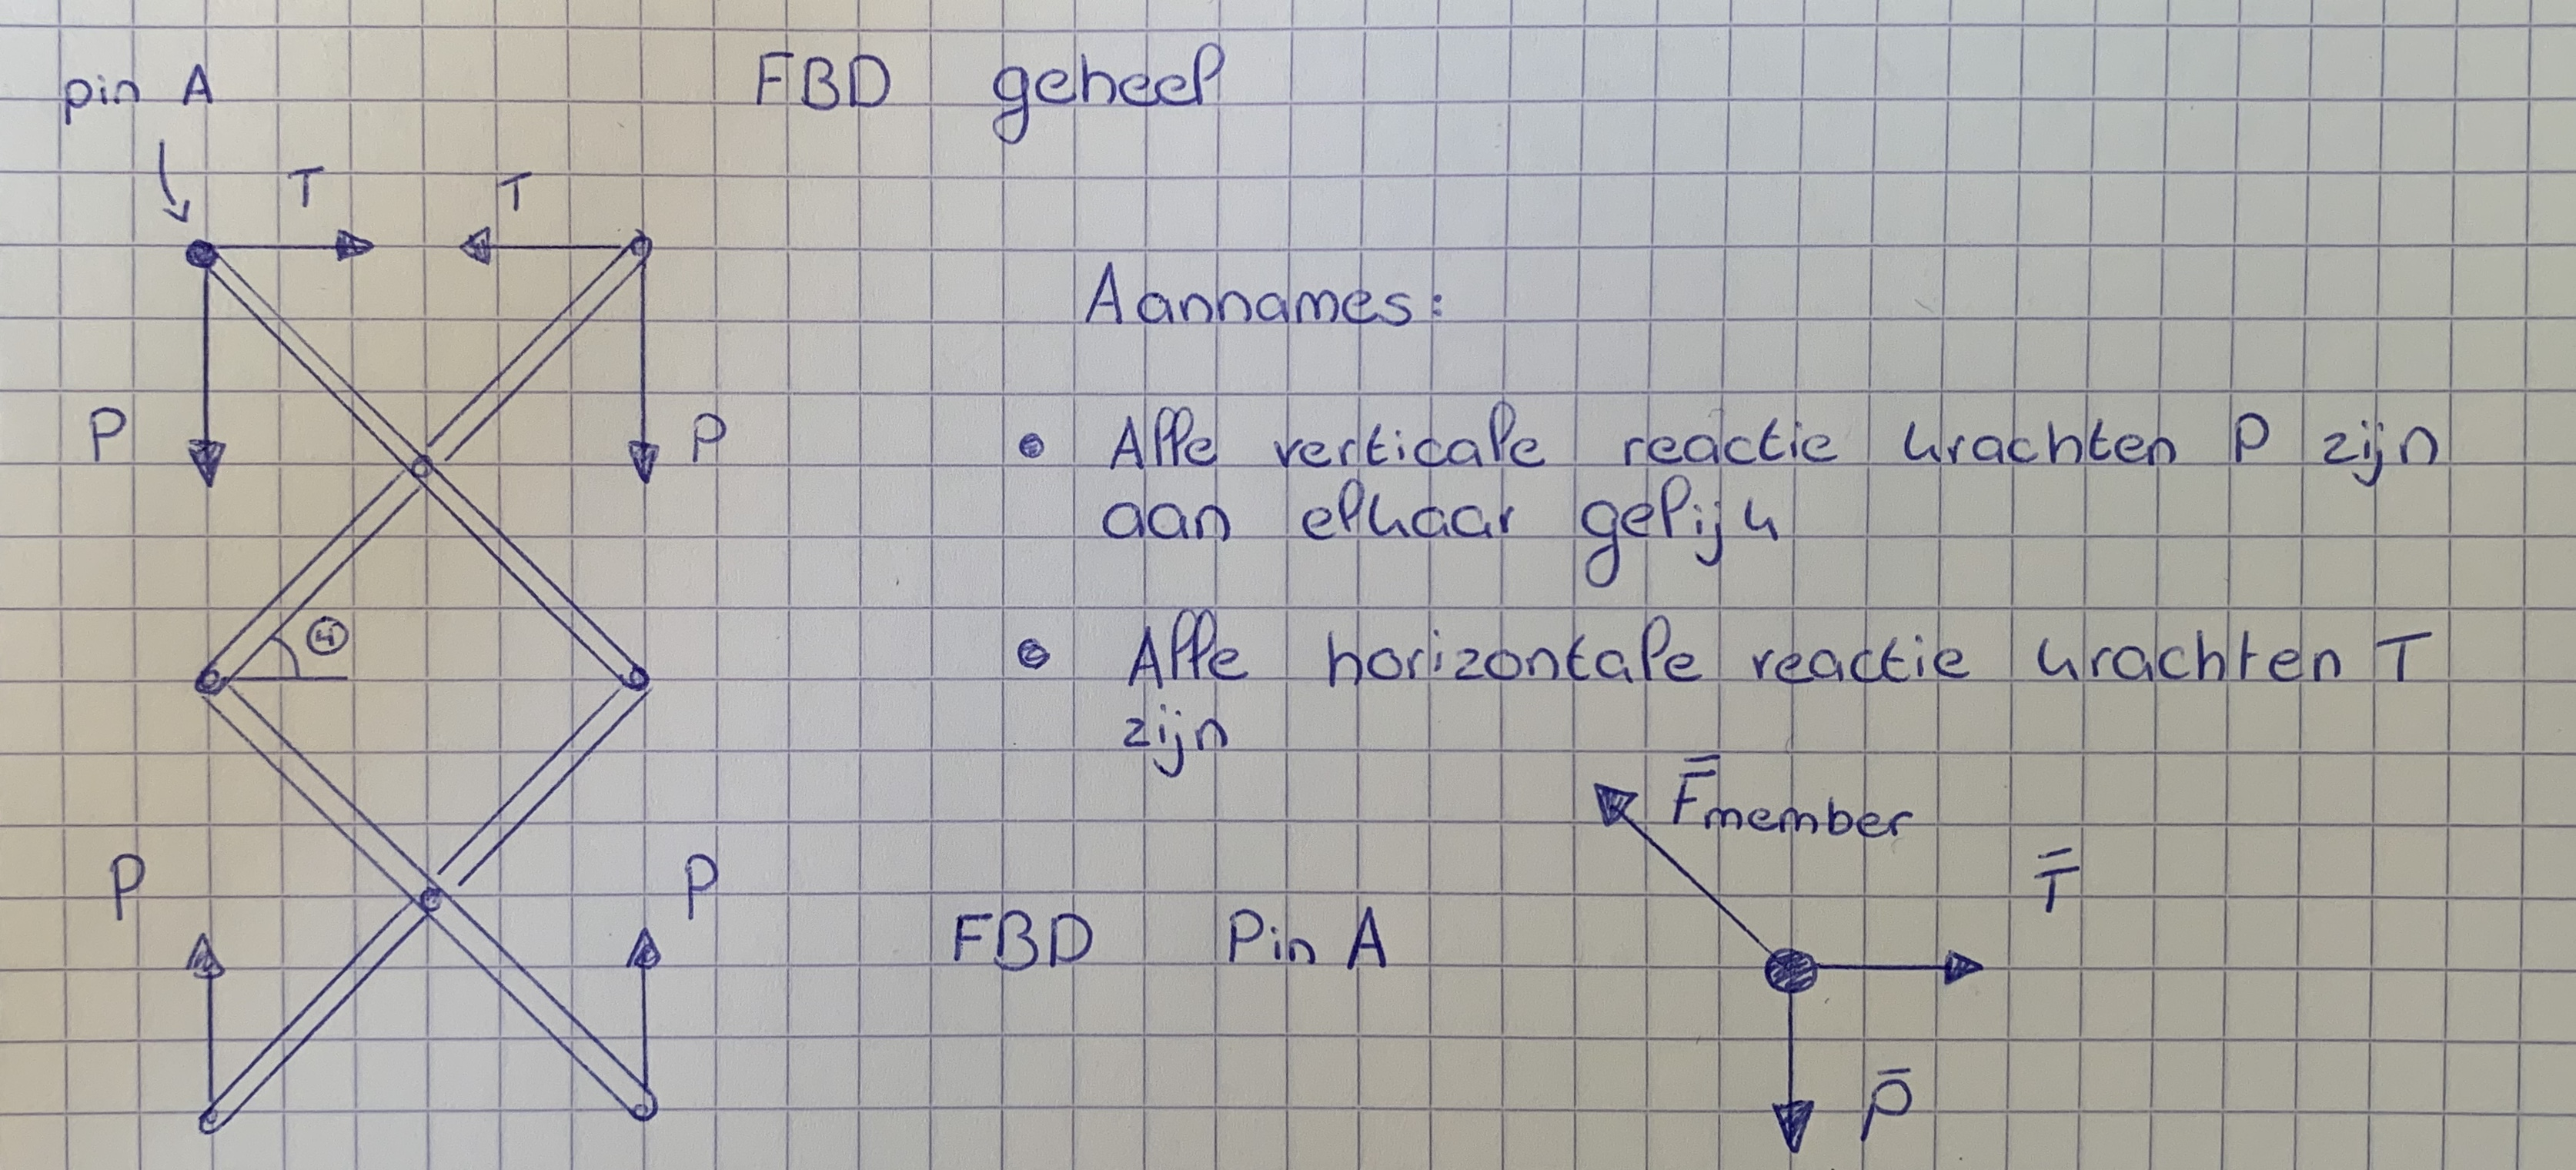
\includegraphics[width = 100mm]{04_conceptdimensionering/member_FBD.jpg}
    \caption{FBD van de schaarlift en pin in een member.}
    \label{fig: FBD_member}
\end{figure}
\vspace{\baselineskip}

\begin{figure}[H]
    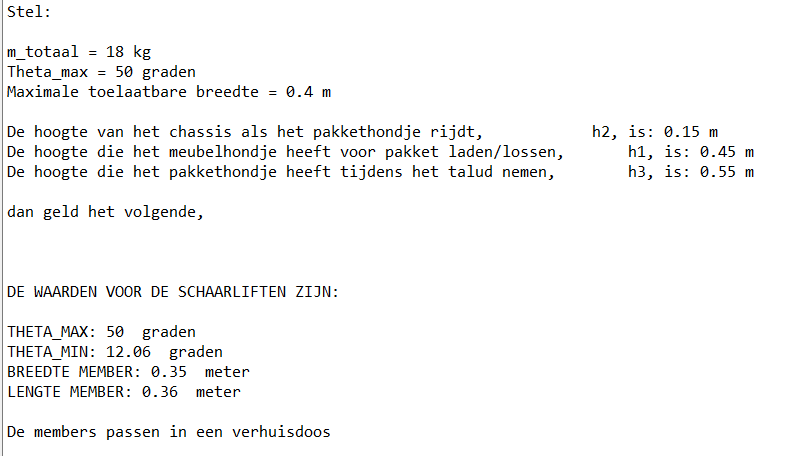
\includegraphics[width = 100mm]{04_conceptdimensionering/Schaarlift_kernel_1.PNG}
    \caption{Kernel van het python script.}
    \label{fig: Kernel_schaarlift_1}
\end{figure}

\begin{figure}[H]
    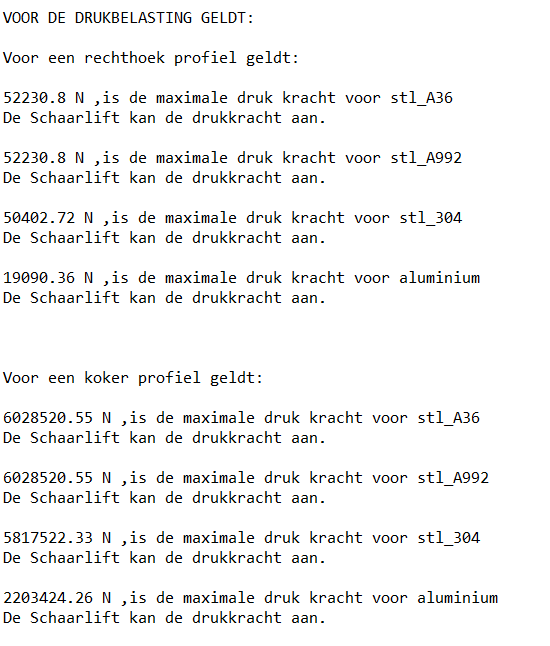
\includegraphics[width = 80mm]{04_conceptdimensionering/Schaar.PNG}
    \caption{Kernel van het pyhton script.}
    \label{fig: Kernel_schaarlift_2}
\end{figure}
\vspace{\baselineskip}

\textbf{De motoren.}\\

\textbf{Het stuursysteem.}\\

\textbf{L-profiel aan de bovenkant van de kar.}\\

\textbf{U-profiel aan de onderkant van de kar.}\\
Er is voor een U-profiel gekozen vanwege de vorm van de belasting. Deze is versimpeld weergegeven in \cref{fig: schets_FBD_uprofiel} te zien. Wanneer de zijkanten als ingeklemd worden beschouwd kan de conclusie worden getrokken dat het onderdeel zowel op buiging als op trek wordt belast. Een geschikt profiel voor dit soort belasting is het U-profiel.\\
Hiermee is een python script geschreven, zie \cref{se: onderkant_u-profiel} in \cref{Cha: Bijlage_F}. Uit dit script is de dimensionering gehaald, zie \cref{fig:u-profiel_constanten}. Het u-profiel is vervolgens berekend op sterkte en stijfheid er is een krachten- en momentenlijn opgesteld (\cref{fig: momentenlijn_onderkant} \& \cref{fig: krachtenlijn_onderkant}). Uit de momenten en krachtenlijn is gebleken dat het u-profiel de krachten kan hebben, zie \cref{fig: kernel_onderkant}.

\begin{figure}[H]
    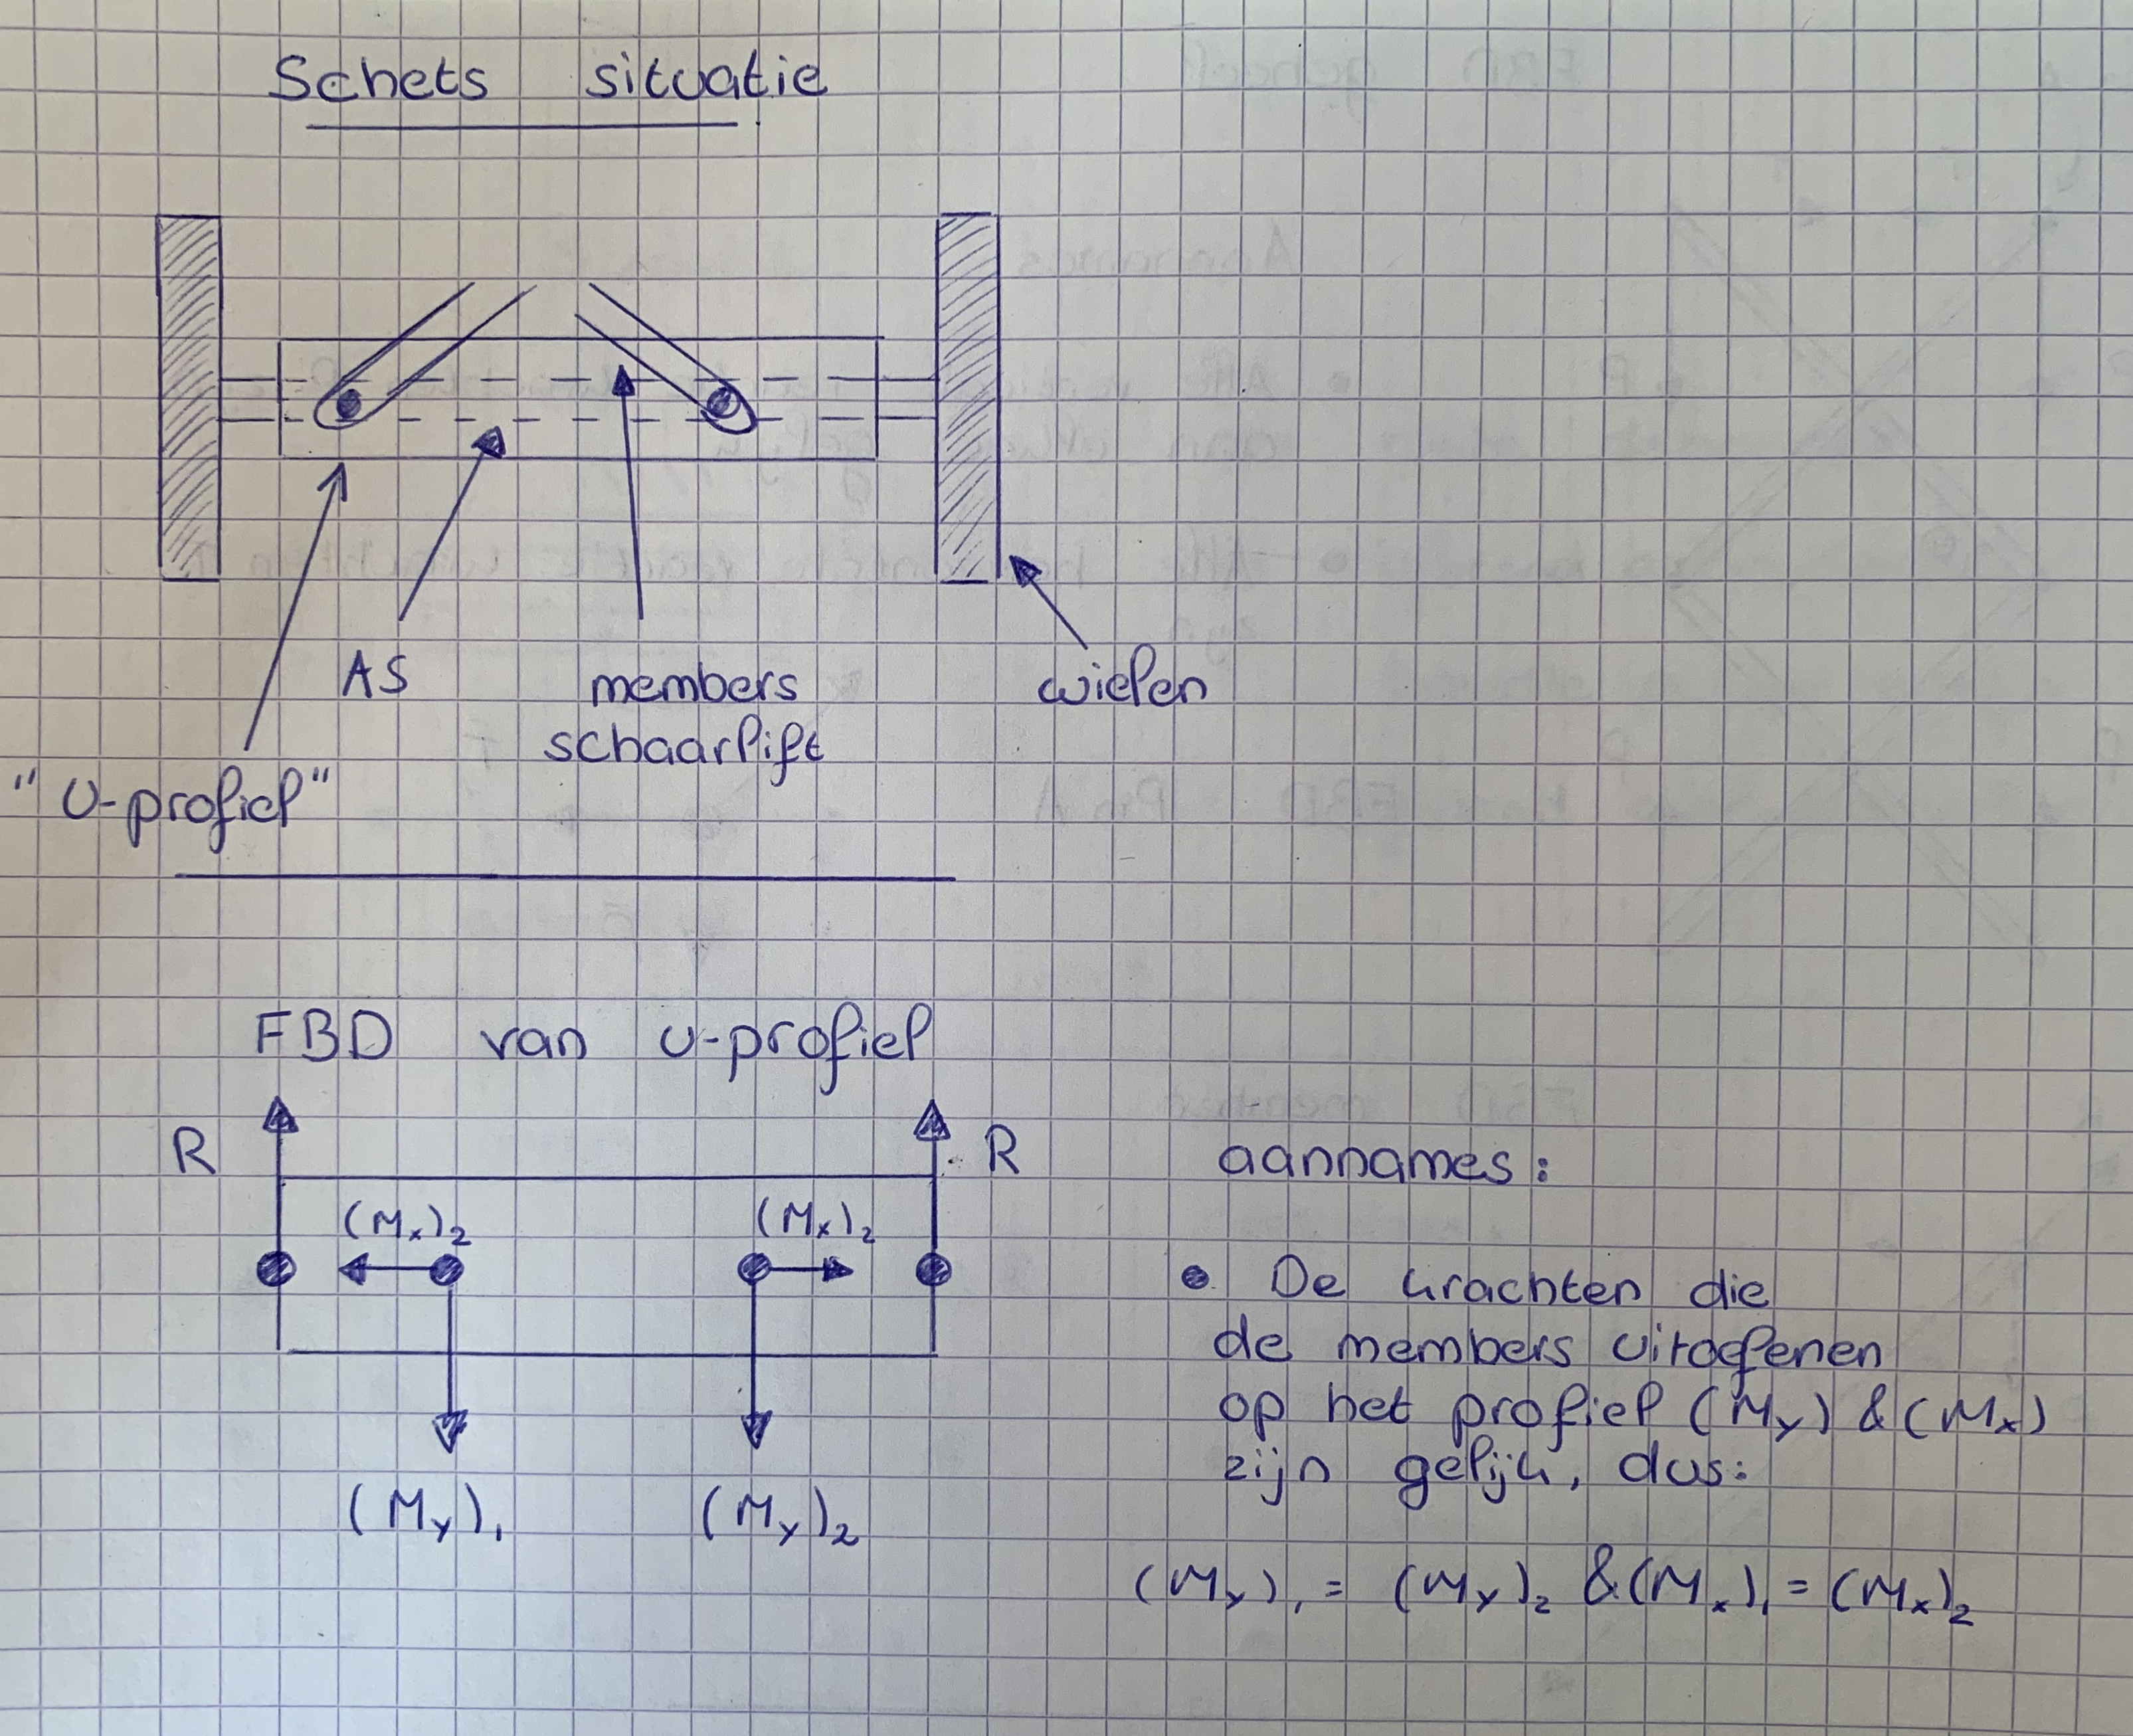
\includegraphics[width = 80mm]{04_conceptdimensionering/U-profiel_tekening.jpg}
    \caption{schets situatie en FBD van u-profiel onderaan de kar.}
    \label{fig: schets_FBD_uprofiel}
\end{figure}
\vspace{\baselineskip}

\begin{figure}[H]
    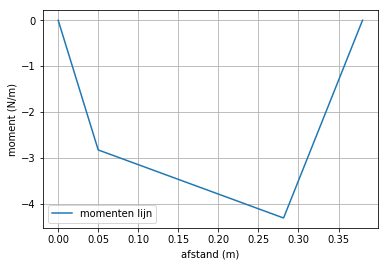
\includegraphics[width = 80mm]{06_bijlage_F/onderkant_u_profiel/momentenlijn_onderkant.png}
    \caption{Momentenlijn van het u-profiel aan de onderkant van de kar.}
    \label{fig: momentenlijn_onderkant}
\end{figure}
\vspace{\baselineskip}

\begin{figure}[H]
    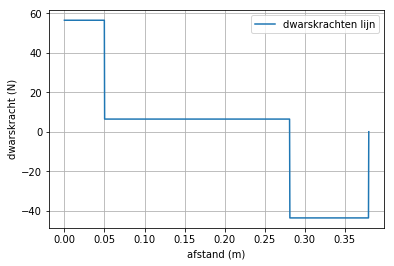
\includegraphics[width = 80mm]{06_bijlage_F/onderkant_u_profiel/krachtenlijn_onderkant.png}
    \caption{Krachtenlijn van het u-profiel aan de onderkant van de kar.}
    \label{fig: krachtenlijn_onderkant}
\end{figure}
\vspace{\baselineskip}

\begin{figure}[H]
    
\includegraphics[width = 120mm]{06_bijlage_F/onderkant_u_profiel/kernel_onderkant.PNG}
    \caption{Kernel van het python script.}
    \label{fig: kernel_onderkant}
\end{figure}
\vspace{\baselineskip}










\section{Maak- en kooplijst}
\label{maaklijst_kooplijst}

Nadat de berekeningen en dimensionering zijn afgerond kunnen de maak- en kooplijsten worden opgesteld. In \cref{fig:maaklijst} staat de maaklijst van de driepoter en in \cref{fig:kooplijst} staat de kooplijst van de driepoter.

\begin{figure}[H]
    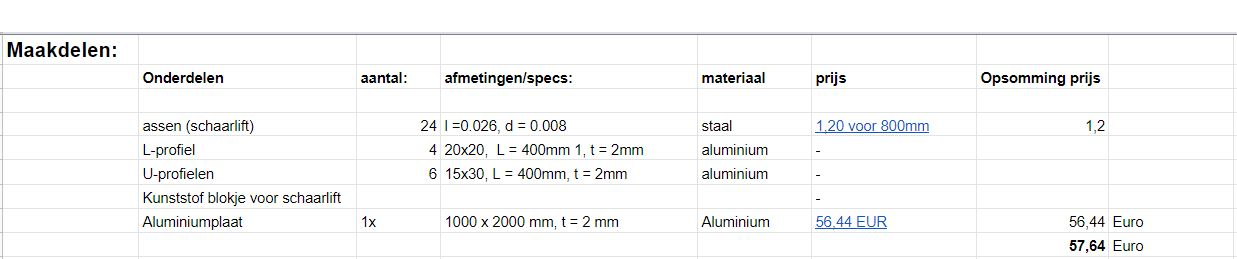
\includegraphics[width = 120mm]{04_conceptdimensionering/Tabel_Maaklijst.JPG}
    \caption{Maaklijst van de Driepoter}
    \label{fig:maaklijst}
\end{figure}

De maaklijst bevat de onderdelen die zelf gefabriceerd kunnen worden, hieronder verstaat men de L-profielen en de U-profielen. Deze profielen worden uit aluminiumplaat gesneden en vervolgens gebogen. 

\vspace{\baselineskip}
\begin{figure}[H]
    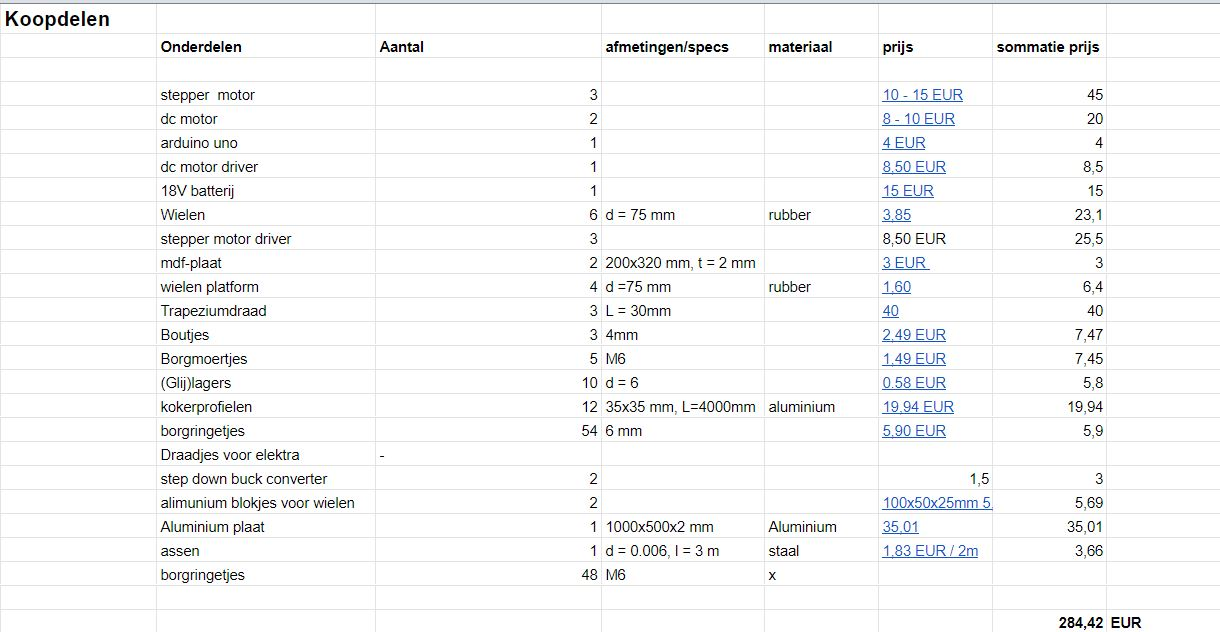
\includegraphics[width = 120mm]{04_conceptdimensionering/Tabel_Kooplijst.JPG}
    \caption{Kooplijst van de Driepoter}
    \label{fig:kooplijst}
\end{figure}

\section{Bestellijst.}
Uit de kooplijst is een selectie gemaakt van onderdelen, die samen maximaal 80 euro kostte. 


\chapter{Vervaardigingsplan}
\label{Vervaardigingsplan}
\textit{In dit hoofdstuk wordt het vervaardigingsplan ontwikkeld. Hier wordt de tijdsplanning en het tijdsverloop voor de assemblage besproken. De volgende vragen worden beantwoord: Hoe komt men aan het benodigde materiaal en gereedschap? Door wie, waar en wanneer wordt er aan het pakkethondje gewerkt?}

\section{Benodigde materialen}
\label{Benodigde_materialen}
In \cref{fig:maaklijst} en \cref{fig:kooplijst} staan de maak- en kooplijsten. Deze onderdelen moeten uiteraard samen worden geassembleerd. De meeste componenten worden vastgemaakt met een schroefverbinding, deze kunnen met de hand of met een moersleutel worden aangedraaid. Andere verbindingen in het pakkethondje zijn lasvebindingen voor de kapjes van de wielen en klinkverbindingen voor smalle ruimten. \\
\vspace{\baselineskip}
Het gereedschap dat nodig is:
\begin{center}
 \begin{tabular}{| l | c | r |}  
 \hline
\textbf{Gereedschap} & \textbf{Beschikbaarheid} \\
  Moersleutel          & IWS                      \\
  Hamer                & IWS                      \\
  Boormachine          & IWS                      \\
  Freesmachine         & IWS                      \\
  Lasapparaat          & IWS                      \\
  Popnageltang         & IWS                      \\
  Lasersnijder         & IWS                      \\
  3D-printer           & IWS/ Zelf beschikbaar    \\
  Smeerolie            & IWS/ Bouwmarkt       \\
  \hline
 \end{tabular}
\end{center}

%\begin{center}
% \begin{tabular}{| l | c | r | }
%  \hline			
%  score: & concept: & punten:\\
%  1 & Inklapper & 184 \\
%  2 & Vierpoter & 180 \\
%  3 & Mantis Car & 174 \\
%  4 & Uitschuiver & 165 \\
%  \hline  
% \end{tabular}
%\end{center}
%\vspace{\baselineskip}
\section{Lasersnijden}
\label{se:lasersnijden}
Een groot deel van de onderdelen worden met een lasersnijder uit aluminium- en staalplaat gesneden. De U-profielen en hoekprofielen worden vervolgens gebogen tot de gewenste vorm. Dit zorgt ervoor dat er minder onderdelen moeten worden besteld en de kosten lager zijn. Ook heeft dit het voordeel dat alle boorgaten van tevoren zijn gemaakt. De onderdelen die moeten worden gelasersneden zijn in Solidworks gemodelleerd en worden in een DXF-bestand naar de IWS gestuurd.

\section{Lassen}
\label{se:Lassen}
Voor het lassen moeten de zogenaamde U-kapjes waar de wielen aan zijn verbonden worden gelast aan de schaarlift, zie \cref{fig:U-kapjes}. Er zijn twee redenen voor het kiezen van een lasverbinding. Ten eerste zullen hier de grootste krachten plaatsvinden. Ten tweede is het lastig om andere verbindingstechnieken zoals boutverbindingen toe te passen omdat de afmetingen te klein zijn om daar met een moersleutel te komen.

\begin{figure}[H]
    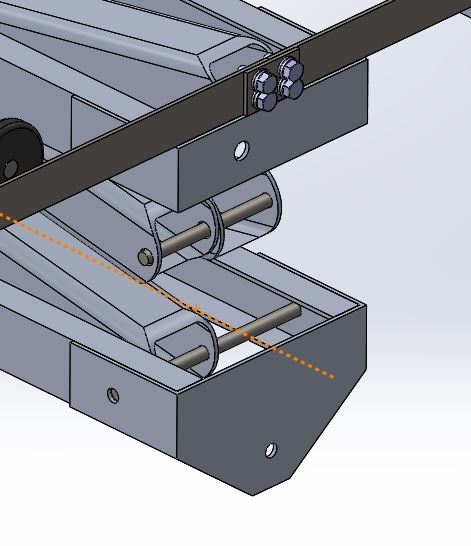
\includegraphics[width = 80mm]{04_vervaardigingsplan/U-kapjes.JPG}
    \caption{U-kapjes, zonder wiel}
    \label{fig:U-kapjes}
\end{figure}

\section{Frezen}
\label{se:Frezen}
Voor het frezen zullen het spindelblokje en de stuurblokjes met een freesmachines worden bewerkt. Dit is omdat deze onderdelen zeer accurate afmetingen hebben die niet kunnen worden besteld. Dit is vooral belangrijk voor de stuurblokjes omdat de precisie van de afmetingen direct invloed hebben op de wendbaarheid van het pakkethondje, zie \cref{fig:stuurblokjes}.


\begin{figure}[H]
    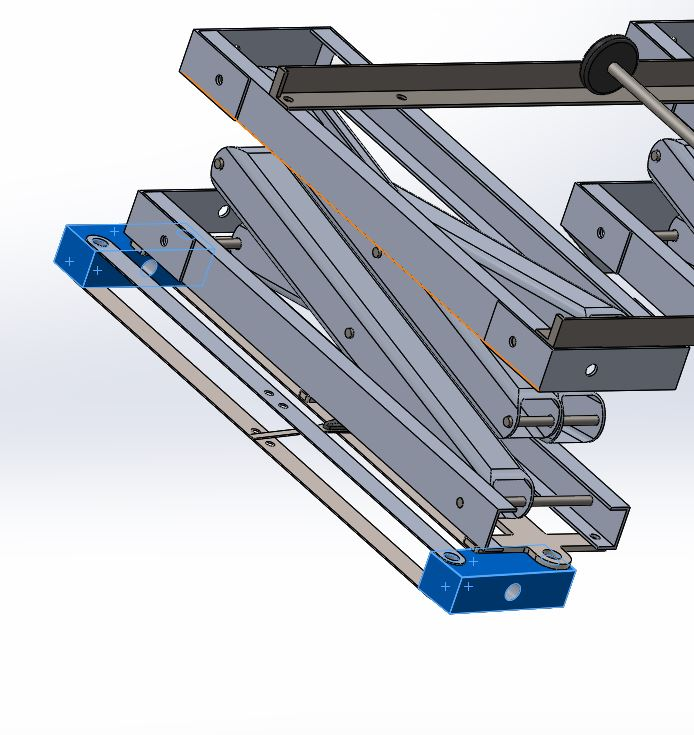
\includegraphics[width = 80mm]{04_vervaardigingsplan/Stuurblokjes.JPG}
    \caption{Stuurblokjes}
    \label{fig:stuurblokjes}
\end{figure}


\section{Overige processen}
\label{se:Overige_processen}
In deze paragraaf worden de overige assemblageprocessen behandeld.
\\
\textbf{Boormachine}\\
De kokerprofielen van de schaarlift bevatten nog geen boorgaten voor de assen, deze zullen dus met een boormachine moeten worden gemaakt in de IWS.
\\
\textbf{3D-printen}\\
De kunststof blokjes aan de bovenkant van de schaarlift zullen worden geprint met een 3D-printer. Deze wordt beschikbaar gesteld door een van de groepsleden.
\\
\textbf{Klinknagels} \\
Voor verbindingen die te smal zijn voor een boutverbinding worden popnagels toegepast. Deze kunnen via één kant worden aangebracht, wat ideaal is voor smalle stukken. Dit is een materiaalgesloten verbinding, wat voordelen en nadelen heeft. Het voordeel van popnagels is dat het gemakkelijk aan te brengen is een zeer sterk is. Het nadeel ervan is dat het niet demontabel is.

\section{Tijdsplanning vervaardiging}
\label{se:planning_vervaardiging}
Er zijn in totaal vijf momenten waar er aan het pakkethondje kan worden gewerkt in de IWS. Hier volgt de planning voor het vervaardigen en assembleren van het pakkethondje:

\begin{table}[H]
\begin{tabular}{| l | l |}
\textbf{IWS moment} & \textbf{Taken}                                                       \\
1                   & Boorgaten maken in kokerprofielen, \newline frezen van belangrijke onderdelen \\
2                   & Schaarliften en platform assembleren                                 \\
3                   & Verder met schaar en platform, lassen, stuursysteem assembleren      \\
4                   & Stuursysteem afronden, geheel in elkaar zetten                       \\
5                   & Geheel in elkaar zetten 
\end{tabular}
\end{table}


\chapter{Prestatie verwachtingen}
\label{Prestatie_verwachtingen}
\textit{In dit hoofdstuk worden de prestaties verwachtingen toegelicht aan de hand van de in \cref{cha:opdrachtanalyse} opgestelde prestatie criteria (\cref{se:PC}) en functionele eisen (\cref{se:PVE}). In \cref{se:presentatie_ontwerp} wordt het ontwikkelde concept gepresenteerd, hier wordt een korte omschrijving van het ontwerp gegeven samen met een afbeelding. In \cref{se:prestatie_en_eigenschappen} worden de verwachte prestaties verteld met eventuele berekeningen om dezen te ondersteunen, ook worden hier de specifieke eigenschappen van het ontwerp toegelicht. In \cref{se:veiligheidsanalyse_prestatieverwachting} wordt een veiligheid-overzicht van het ontwerp gepresenteerd.}

\section{Presentatie van het ontwerp}
\label{se:presentatie_ontwerp}

De Driepoter is een ontwerp dat in staat is om over obstakels heen te stappen door middel van zijn inklapbare poten. Zoals te zien is in \cref{fig:De_driepoter_Prestatie_analyse} is de Driepoter in staat om de schaarliften die hij aan de onderkant van het chassis heeft in te klappen en uit te klappen. De Driepoter kan het pakket ontvangen door middel van een rol-baar plateau, dit zorgt ervoor dat de Drieklapper een verstelbaar zwaarte punt heeft wat handig is voor het nemen van een talud. Eenmaal wanneer de Driepoter een bocht moet maken kan hij zien voorste wielen draaien en net als een auto een bocht maken.\\

\vspace{\baselineskip}
\begin{figure}[H]
    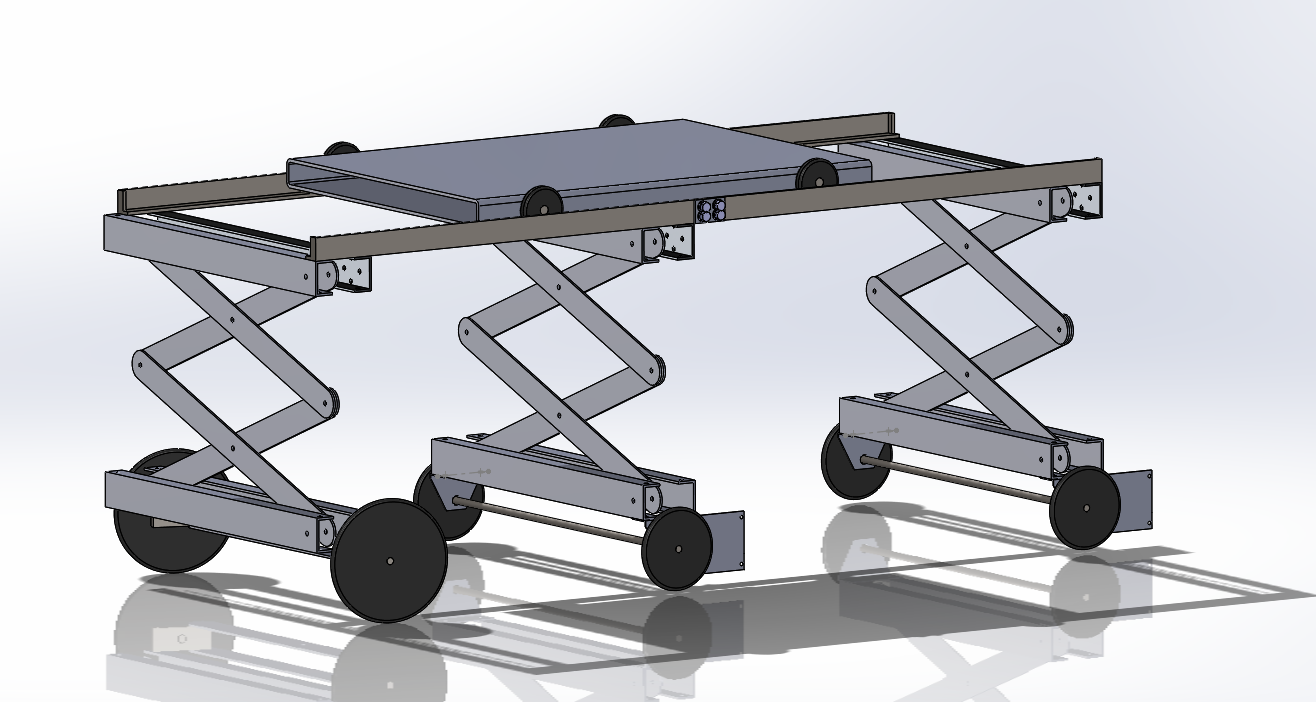
\includegraphics[width = 120mm]{04_gekozenconcept/eindconcept.png}
    \caption{de Driepoter}
    \label{fig:De_driepoter_Prestatie_analyse}
\end{figure}


\section{Verwachte eigenschappen en prestaties}
\label{se:prestatie_en_eigenschappen}
Hier worden de prestaties en de eigenschappen van de Driepoter besproken en onderbouwt door middel van berekeningen en bronnen. De mogelijke prestaties zijn aan de hand van de prestatie criteria en het programma van eisen in \cref{cha:opdrachtanalyse} opgesteld. De gekozen prestaties en eigenschappen die moet worden bepaald zijn: De dynamische en statische stabiliteit, het balans van het pakketje, de benodigde hoeveelheid energie voor het nemen van de hindernis baan en de tijd die het pakket hondje kost voor het nemen van de hindernisbaan. 

\subsection{De stabiliteit}
Erg belangrijk is het voor het pakkethondje dat hij niet omvalt tijdens het versnellen, afremmen of het nemen van een talud. De stabiliteit is in twee delen verdeeld: de dynamische stabiliteit en de statische stabiliteit. Onder de dynamische stabiliteit valt het versnellen en remmen van het pakkethondje en onder de statische stabiliteit valt het nemen van een talud en het rijden van het pakkethondje.\\
Voordat er berekeningen worden gedaan moeten een aantal parameters worden bepaalt:

\begin{itemize}
    \item \textbf{De hoogte van het massamiddelpunt bij verschillende tijdstippen in het nemen van de hindernisbaan}. De hoogte van het massa middelpunt als de schaarliften volledig zijn ingeklapt is 
    \item \textbf{Het steunvlak}. Deze wordt bepaald door de 3 paar wielen aan de onderkant van de schaarlift. De wielen staan 530 mm en 350mm van elkaar af. 
    \item Eventuele externe krachten of veranderingen in deze krachten
    \item Maximale hoek van talud 1
    \item De maximale versnelling
\end{itemize}
\vspace{\baselineskip}

\subsection{Balans van het pakketje}

\subsection{Benodigde hoeveelheid energie}

\subsection{Snelheid van het nemen van de hindernisbaan}


\section{veiligheidsanalyse}
\label{se:veiligheidsanalyse_prestatieverwachting}



\chapter{Conclusie}
\label{cha:conclusie}
Het doel van dit rapport was het ontwerpen van een 'Pakkethondje' dat een gewicht van 10 kg over een hindernisbaan kan transporteren. De belangrijkste criteria bij dit ontwerp was het kunnen overnemen van een obstakel. 

\vspace{\baselineskip}
Tijdens het ontwerpproces zijn vier kansrijke ontwerpen ontwikkeld: de 'Mantis Car', de 'Uitschuiver', de 'Inklapper' en de 'Vierpoter'. Van deze ontwerpen zijn prototypes gemaakt die werden getest op de prestatiecriteria. Uit de testen bleek dat het meest kansrijke ontwerp een samenstelling is van de vier prototypes. Er is gekozen voor het mechanisme van de driepoot waarbij de schaarliften van de uitschuiver worden gebruikt. Dit eindontwerp gaat onder de naam 'Driepoter' en is te zien in \cref{fig:eindconcept}

\begin{wrapfigure}{r}{5.5cm}
    \centering
    \includegraphics[width = 50mm]{05_conclusie/eindconcept.jpg}
    \caption{Solidworksmodel van het eindconcept}
    \label{fig:eindconcept}
\end{wrapfigure}

\vspace{\baselineskip}
De voornaamste reden voor het kiezen van de schaarlift is dat het stabieler is dan de andere deelontwerpen. Een tweede reden voor het kiezen van de schaarlift is in verband met de lengte van het voertuig. Het gebruik van inklapbare poten vereist een zeer lange kar, wat zorgt voor problemen tijdens het sturen.  Een andere reden voor de schaarlift is de veelzijdigheid van het ontwerp. Schaarliften kunnen gemakkelijk een verticale beweging opdoen, waardoor het over de meeste obstakels kan rijden. Deze eigenschap missen de andere concepten.

Hoewel de schaarlift de beste keuze blijkt te zijn, zijn er nog een aantal aanbevelingen voor volgende rapporten. Aanbeveling 1 is het onderzoeken van de schaarliften en of ze op de manier hoe ze in dit concept zijn geconstrueerd ook wel echt ideaal zijn. Misschien is er nog een betere versie van de schaarlift waardoor het eindconcept nog verder verbeterd zou kunnen worden. Aanbeveling 2 zou het onderzoeken van de duurzaamheid van het eindconcept kunnen zijn. Zijn er misschien betere motoren en/of materialen die de gevraagde functies vervullen en ook beter zijn voor het milieu zou een vraag kunnen zijn die kan volgen op dit rapport.



% Refereer naar de MCA!! Gewicht, kosten, snelheid, duurzaamheid, etc.




\renewcommand\bibname{Literatuurlijst}

\printbibliography[heading=bibnumbered]

\appendix

%% Zet hier je bijlagen neer

\chapter{ACCREX}
\label{cha:bijlage_E}

\begin{figure}[H]
    \centering
    \includegraphics[width = 180mm, angle=270]{06_bijlage_E/ACCREx_tabel_g.PNG}
    \caption{ACCREx tabel.}
    \label{fig:Accrex_tabel}
\end{figure}

\chapter{Morfologische kaart}
\label{ap:bijlage_A}


\begin{figure}
    \includegraphics[width = 180mm, angle = 270]{06_bijlage_A/morf_kaart.png}
    \caption{De morfologische kaart.}
    \label{fig:morf_kaart}
\end{figure}

\chapter{Gewogen criteria methode}
\label{ch:gewogen_criteria_methode}
\newpage{}

\begin{figure}[H]
    \includegraphics[width=180mm, angle = 270]{06_bijlage_B/wegingen.png}
    \caption{De wegingen van de prestatiecriteria gegeven in \cref{se:PVE}}
    \label{fig:wegingen}
\end{figure}

\begin{figure}[H]
    \includegraphics[width=180mm, angle = 270]{gegeven_scores_goed.PNG}
    \caption{De  scores van vier uitgewerkte concepten}
    \label{fig:conceptscores}
\end{figure}




\chapter{Ingewonnen informatie}
\label{cha:bijlage_C}

\section{Elektra prijzen}

\subsection{Accu prijzen}
\vspace{\baselineskip}

\textbf{Specificaties, \cite{Conrad}}\\

Model: \textbf{Black-Decker-PS130-A9252}\\
Voltage:	12 V	\\
Afmetingen:	92 x 81 x 102 mm \\
Kleur:	zwart	\\
Type:	Ni-MH \\
Capaciteit:	2.100 mAh \\
\vspace{\baselineskip}

Model: \textbf{UltraCell-UCG9-12-Deep-Cycle-Gel} \\
Voltage:	12 V	\\
Afmetingen:	151 x 65 x 99 mm \\
Capaciteit:	9.000 mAh	\\
Type:	Sealed Lead Acid - AGM \\
\vspace{\baselineskip}

Model:  \textbf{Associated-NS300D37C006} \\
Voltage:	7,2 V	\\
Type:	Ni-MH\\
Capaciteit:	3.000 mAh	\\
Output connector:	standard tamiya \\
Afmetingen:	130 x 46 x 24 mm \\

\subsection{Elektromotor prijzen}
\vspace{\baselineskip}

\textbf{Specificaties, \cite{Conrad}}
\vspace{\baselineskip}

Model: \textbf{Joy-it Stappenmotor NEMA-17-01 NEMA-17-01 0.4} \\
Voedingsspanning	2.8 V \\
Hoek	1.8 °\\
Moment bij stand	0.4 Nm \\
Max. fasestroom	1.68 A \\
As-Ø	5 mm \\
Aslengte	22 mm \\
Fabrikantnr.	NEMA-17-01 \\
Type	NEMA-17-01 \\
Breedte	47 mm \\
Nominale spanning	2.8 V \\
\vspace{\baselineskip}

Model: \textbf{Joy-it Stappenmotor 0.15 Nm 0.75 mA As-diameter} \\
Hoek	1,8 ° \\
Moment bij stand	0.15 Nm \\
As-Ø	4,5 mm \\
Aslengte	16 mm \\
Breedte	35 mm \\
Nominale stroom	0.75 mA \\
Nominale spanning	4.35 V \\
Fasen	2 \\
As-Ø	4.5 mm \\
Motorlengte	35 mm \\
\vspace{\baselineskip}

Model: \textbf{Brushed universele elektromotor Igarashi N2738-48GF.} \\
Onbelast toerental	16000 omw/min \\
Afgiftevermogen	17 W \\
Voedingsspanning	3 - 9 V/DC \\
Nullast-stroom	0,6 A \\
Belast toerental	13600 omw/min \\
Fabrikantnr.	2738-048-GFC-3 \\
Max. draaimoment	12 Nmm \\
Gem. stroomverbruik	3.5 A \\
Efficiëntie	68 % \\
Aslengte	37.8 mm \\
\vspace{\baselineskip}

\section{Bestaande mechanismes met dezelfde functie.}
\vspace{\baselineskip}

IDA Motor Controller: \\
The IDA motor controller consists of two printed-circuit boards located in the lower Payload Electronics Box (PEB) and provides power conditioning, motor voltage control and drivers, grapple heater drivers, joint encoder counting, and analog-to-digital conversion of potentiometer voltages, temperature sensor voltages, motor currents, and heater current. The PEB provides the interface to the Lander Command and Data Handling (C \& DH) computer over a serial link. Firmware running on the IDA motor controller microprocessor provides for low-level motor command execution to move the joints to the specified positions, grapple heater command execution, analog-to-digital calibration, and sensor monitoring. \cite{r.g._bonitz_nguyen_kim_bonitz_folkner_golombek_olson_spohn_grott_et_al._1970}
\vspace{\baselineskip}

\section{Mogelijke stuursystemen.}
\vspace{\baselineskip}

\begin{figure}[H]
    \includegraphics[width=100mm]{06_bijlage_C/ackermann.PNG}
    \caption{Stuursysteem, \cite{king-hele_2002}}
    \label{fig:conceptscores9}
\end{figure}

\vspace{\baselineskip}

\begin{figure}[H]
    \includegraphics[width=100mm]{06_bijlage_C/Ackermann2.PNG}
    \caption{Stuursysteem, \cite{king-hele_2002}}
    \label{fig:conceptscores0}
\end{figure}


\input{06_bijlage_D/Bijlage_D}

\chapter{Python scripts}
\label{Cha: Bijlage_F}

\section{wielassen.}
\label{Se: bijlage_F wielassen}
\begin{figure}[H]
    \centering
    \includegraphics[width = 120mm]{06_bijlage_F/As_script/Doorbuiging_as_constanten.PNG}
    \caption{Python script, doorbuiging assen, constanten.}
    \label{fig:python_d.a._constanten}
\end{figure}

\vspace{\baselineskip}

\begin{figure}[H]
    \centering
    \includegraphics[width = 120mm]{06_bijlage_F/As_script/Doorbuiging_as_krachten_analyse.PNG}
    \caption{Python script, doorbuiging assen, krachten analyse.}
    \label{fig:python_d.a._krachtenanalyse}
\end{figure}

\vspace{\baselineskip}

\begin{figure}[H]
    \centering
    \includegraphics[width = 120mm]{06_bijlage_F/As_script/Doorbuiging_as_functies.PNG}
    \caption{Python script, doorbuiging assen, functies van dwarskrachten en momenten.}
    \label{fig:python_d.a._functies}
\end{figure}

\vspace{\baselineskip}

\begin{figure}[H]
    \centering
    \includegraphics[width = 120mm]{06_bijlage_F/As_script/Doorbuiging_as_forloop.PNG}
    \caption{Python script, doorbuiging assen, for-loop.}
    \label{fig:python_d.a._forloop}
\end{figure}

\vspace{\baselineskip}

\begin{figure}[H]
    \centering
    \includegraphics[width = 120mm]{06_bijlage_F/As_script/Doorbuiging_as_plottenprinten.PNG}
    \caption{Python script, doorbuiging assen, plots en print waarden.}
    \label{fig:python_d.a._plotsenprints}
\end{figure}
\vspace{\baselineskip}

\section{Schaarliften}
\label{se: bijlage_F schaarliften}
\vspace{\baselineskip}

\begin{figure}[H]
    \centering
    \includegraphics[width = 120mm]{04_conceptdimensionering/Constanten_schaarlift.PNG}
    \caption{Python script, schaarliften.}
    \label{fig:schaarliften_constanten}
\end{figure}
\vspace{\baselineskip}

\begin{figure}[H]
    \centering
    \includegraphics[width = 120mm]{06_bijlage_F/Schaarlift_script/berekeningen_schaarlift.PNG}
    \caption{Python script, schaarliften.}
    \label{fig:schaarliften_berekeningen}
\end{figure}
\vspace{\baselineskip}

\begin{figure}[H]
    \centering
    \includegraphics[width = 120mm]{06_bijlage_F/Schaarlift_script/prints1_schaarlift.PNG}
    \caption{Python script, schaarliften.}
    \label{fig:schaarliften_sript1}
\end{figure}
\vspace{\baselineskip}

\begin{figure}[H]
    \centering
    \includegraphics[width = 120mm]{06_bijlage_F/Schaarlift_script/prints2_schaarlift.PNG}
    \caption{Python script, schaarliften.}
    \label{fig:schaarliften_sript2}
\end{figure}
\vspace{\baselineskip}

\section{U-profiel aan de onderkant van de kar}
\label{se: onderkant_u-profiel}

\begin{figure}[H]
    \centering
    \includegraphics[width = 120mm]{06_bijlage_F/onderkant_u_profiel/constanten_onderkant.PNG}
    \caption{Python script, u-profiel.}
    \label{fig:u-profiel_constanten}
\end{figure}
\vspace{\baselineskip}

\begin{figure}[H]
    \centering
    \includegraphics[width = 120mm]{06_bijlage_F/onderkant_u_profiel/krachtenanalyse_onderkant.PNG}
    \caption{Python script, u-profiel.}
    \label{fig:u-profiel_krachtenanalyse}
\end{figure}
\vspace{\baselineskip}

\begin{figure}[H]
    \centering
    \includegraphics[width = 120mm]{06_bijlage_F/onderkant_u_profiel/formules_onderkant.PNG}
    \caption{Python script, u-profiel.}
    \label{fig:u-profiel_formules}
\end{figure}
\vspace{\baselineskip}

\begin{figure}[H]
    \centering
    \includegraphics[width = 120mm]{06_bijlage_F/onderkant_u_profiel/forloop_onderkant.PNG}
    \caption{Python script, u-profiel.}
    \label{fig:u-profiel_forloop}
\end{figure}
\vspace{\baselineskip}

\begin{figure}[H]
    \centering
    \includegraphics[width = 120mm]{06_bijlage_F/onderkant_u_profiel/print2_onderkant.PNG}
    \caption{Python script, u-profiel.}
    \label{fig:u-profiel_print}
\end{figure}
\vspace{\baselineskip}








\chapter{Specificaties koop delen}
\label{cha:Bijlage_G}

\textbf{Onderdeel}: 18V Batterij \\
\textbf{Naam}: B07M7JW421\\
\textbf{Website}: www.amazon.com\\
\textbf{Specificaties}:\\
Maat: meer dan 4,4cm / 1,73" x3,1cm / 1,22"\\
\[ ombouw: 1 cm = 0,3937 ", 1 " = 2,54 cm \] \\
Accuspanning: 18 V.\\
Nominaal vermogen: 3000mAh\\
Compatibel: voor Makita BL1840 BL1815 BL1830\\
\textbf{Bron}: \cite{amazon.nl}
\vspace{\baselineskip}


\textbf{Onderdeel}: Glijlagers\\  
\textbf{Naam}: igus GFM-0608-06 Glijlager\\
\textbf{Website}: https://www.conrad.nl/\\
\textbf{Specificaties}: \\
Binnendiameter 6mm\\
\textbf{Bron}: \cite{electronic}\\
\vspace{\baselineskip}

\textbf{Onderdeel}: Kokerprofielen  \\
\textbf{Naam}: Aluminium vierkante buis / koker \\
\textbf{Website}: https://www.aluminiumopmaat.nl/ \\
\textbf{Specificaties}: \\
Lengte: 4000mm \\
Breedte: 35mm \\
Hoogte: 35mm \\
\textbf{Bron}: \cite{aluminium op maat}\\
\vspace{\baselineskip}

\textbf{Onderdeel}: Wielen onderkant pakket hondje \\
\textbf{Naam}: ZWE100P2T2P0N \\
\textbf{Website}: www.zwenkwielen.net \\
\textbf{Specificaties}: \\
Diameter wiel: 100 mm \\
Breedte wiel: 32 mm \\
Materiaal wiel: TPR (Streeploos thermo plastisch rubber)\\ 
Hardheid rubber: 95 Shore \\
Materiaal velg: Kunststof polypropyleen \\
Draagvermogen: 100 kg\\
\textbf{Bron}: \cite{zwenkwielen_kopen_koop_nu_voordelig_ieder_zwenkwiel_online}

\textbf{Onderdeel}: Borgringen \\
\textbf{Naam}: DRESSELHAUS Borgring 6 mm DIN 6799 staal \\
\textbf{Website}: https://www.hornbach.nl/ \\
\textbf{Specificaties}: \\
Diameter: 6mm \\
\textbf{Bron}: \cite{hornbach}\\

\textbf{Onderdeel}: Wielen platform pakket hondje\\
\textbf{Naam}:Meubel zwenkwiel 50 mm - M3-50\\
\textbf{Website}: www.wielenoutlet.com\\
\textbf{Specificaties}:\\
Diameter: 50 mm\\
Bandbreedte: 20 mm\\
Draagvermogen: 40 kg\\
Totale hoogte: 70 mm\\
Soort wiel: Zwenkwiel - topplaat\\
\textbf{Bron}: \cite{wielenoutlet}\\

\textbf{Onderdeel}: Aluminium blokjes \\
\textbf{Naam}: Aluminium Blok 100x50x25mm \\
\textbf{Website}: https://www.ijzershop.nl/ \\
\textbf{Specificaties}: \\
Lengte: 100mm \\
Hoogte: 50mm \\
Breedte: 25mm \\
\textbf{Bron}: \cite{ijzershop.nl} \\
\vspace{\baselineskip}

\textbf{Onderdeel}: As \\
\textbf{Naam}: Stalen Massief Rond 6mm\\
\textbf{Website}: https://www.ijzershop.nl/\\
\textbf{Specificaties}:\\
Diameter: 6mm\\
\textbf{Bron}: \cite{ijzershop.nl}\\
\vspace{\baselineskip}

\textbf{Onderdeel}: Trapeziumdraad\\
\textbf{Naam}: Leadscrew, TR8x2, 8 mm - 100 cm\\
\textbf{Website}: www.123-3D.nl\\
\textbf{Specificaties}:\\
Diameter:	8 mm\\	
Lengte:	100 cm\\
\textbf{Bron}: \cite{123}\\
\vspace{\baselineskip}\\

\textbf{Onderdeel}: Bouten\\
\textbf{Naam}:GAMMA metaalschroef M4 x 20mm cilinderkop verzinkt 15 stuks\\
\textbf{Website}: www.gamma.nl\\
\textbf{Specificaties}:\\
Productsoort: Metaalschroef\\
Productnummer: 458192\\
Gewicht product: 50 gr\\
Hoogte product: 2.0 cm\\
Lengte product: 4 mm\\
Breedte product: 4 mm\\
Type(nummer): M4x20mm cilinderkop verzinkt\\
Afwerking: Verzinkt\\
Type: Metaalschroefbout\\
Diameter: 4.0 mm\\
Lengte: 20.0 mm\\
Technische kenmerken: Metrische maat, M4\\
\textbf{Bron}: \cite{gamma}
\vspace{\baselineskip}

\textbf{Onderdeel}: Borgmoertjes \\
\textbf{Naam}: GAMMA borgmoer M5 verzinkt \\
\textbf{Website}: https://www.gamma.nl/ \\
\textbf{Specificaties}: \\
Gewicht product: 16 gr \\
Hoogte product: 1.0 cm \\
Lengte product: 5 mm \\
Breedte product: 1.0 cm \\
Type(nummer): M5 Verzinkt \\
Merk: GAMMA \\
Ecocheque: Nee \\
\textbf{Bron}: \cite{gamma} \\
\vspace{\baselineskip} \\






\thumbfalse

\end{document}
